%\documentclass[pdflatex,en,11pt]{aghdpl}
\documentclass[en]{aghdpl}
\usepackage[english]{babel}
\usepackage{polski}
\usepackage[utf8]{inputenc}

\usepackage[backend=biber,
style=numeric,
%bibencoding=ascii,
%style=reading
giveninits=true
]{biblatex}
\renewbibmacro{in:}{%
    \ifentrytype{article}{}{\printtext{\bibstring{in}\intitlepunct}}}

\addbibresource{bibliografia.bib}

\DeclareNameAlias{sortname}{last-first}
\DeclareNameAlias{default}{last-first}

% dodatkowe pakiety
\usepackage{enumerate}
\usepackage{listings}
\usepackage{float}
\usepackage[binary-units=true]{siunitx}
\usepackage{hyperref}
\usepackage[acronym,nomain,toc]{glossaries}
\usepackage{multirow}
\usepackage{colortbl}
\usepackage{hhline}
\usepackage{lscape}
\usepackage{csquotes}

% \lstloadlanguages{TeX}

\lstset{
  literate={ą}{{\k{a}}}1
           {ć}{{\'c}}1
           {ę}{{\k{e}}}1
           {ó}{{\'o}}1
           {ń}{{\'n}}1
           {ł}{{\l{}}}1
           {ś}{{\'s}}1
           {ź}{{\'z}}1
           {ż}{{\.z}}1
           {Ą}{{\k{A}}}1
           {Ć}{{\'C}}1
           {Ę}{{\k{E}}}1
           {Ó}{{\'O}}1
           {Ń}{{\'N}}1
           {Ł}{{\L{}}}1
           {Ś}{{\'S}}1
           {Ź}{{\'Z}}1
           {Ż}{{\.Z}}1
}

\newcommand{\rad}{\radian}
\newcommand{\iic}{$I^2C$}
\newcommand{\uA}{\micro\ampere}
\newcommand{\mA}{\milli\ampere}
\newcommand{\uV}{\micro\volt}
\newcommand{\mV}{\milli\volt}
\newcommand{\Hz}{\hertz}
\newcommand{\kHz}{\kilo\hertz}
\newcommand{\MHz}{\mega\hertz}
\newcommand{\bps}{\bit / \second}
\newcommand{\Bps}{\byte / \second}
\newcommand{\kbps}{\kilo\bps}
\newcommand{\kBps}{\kilo\Bps}
\newcommand{\Mbps}{\mega\bps}
\DeclareSIUnit{\belmilliwatt}{Bm}
\DeclareSIUnit{\belisotropic}{Bi}
\DeclareSIUnit{\dBm}{\deci\belmilliwatt}
\DeclareSIUnit{\dBi}{\deci\belisotropic}
\DeclareSIUnit{\ppm}{ppm}

\usepackage{array}
\newcolumntype{L}[1]{>{\raggedright\let\newline\\\arraybackslash\hspace{0pt}}m{#1}}
\newcolumntype{C}[1]{>{\centering\let\newline\\\arraybackslash\hspace{0pt}}m{#1}}
\newcolumntype{R}[1]{>{\raggedleft\let\newline\\\arraybackslash\hspace{0pt}}m{#1}}

\makeatletter
\let\ps@plain\ps@fancy
\makeatother

%---------------------------------------------------------------------------

\author{Grzegorz Gajoch}
\shortauthor{G. Gajoch}

\course{Elektronika i Telekomunikacja}

\titlePL{System komunikacji satelity PW-Sat2}
\titleEN{PW-Sat2 satellite communication system}

\shorttitlePL{System komunikacji satelity PW-Sat2} % skrócona wersja tytułu jeśli jest bardzo długi
\shorttitleEN{PW-Sat2 satellite communication system}

\thesistypePL{Praca dyplomowa magisterska}
\thesistypeEN{Master Thesis}

\supervisorPL{dr inż. Cezary Worek}
\supervisorEN{Cezary Worek Ph.D}

\date{2019}

\departmentPL{Katedra Elektroniki}
\departmentEN{Department of Electronics}

\facultyPL{Wydział Informatyki, Elektroniki i Telekomunikacji}
\facultyEN{Faculty of Computer Science, Electronics and Telecommunications}

\acknowledgements{}

\setlength{\cftsecnumwidth}{10mm}
%---------------------------------------------------------------------------

\begin{document}

\titlepages
\tableofcontents
\clearpage

\chapter{Abbreviations}
\vspace{-1cm}
\begin{itemize}
    \setlength\itemsep{-0.5em}
    \item    \textbf{ADCS}      --    Attitude Determination And Control System
    \item    \textbf{AFSK}      --    Audio Frequency Shift Keying
    \item    \textbf{AM}      --    Amplitude Modulation
    \item    \textbf{ANTs}      --    Antenna Module
    \item    \textbf{BPSK}      --    Binary Phase Shift Keying
    \item    \textbf{CAN}      --    Controller Area Network
    \item    \textbf{COMM}      --    Communication Module
    \item    \textbf{CRC}      --    Cyclic Redundancy Code
    \item    \textbf{EIRP}      --    Equivalent Isotropical Radiated Power
    \item    \textbf{EPS}      --    Electrical Power Supply
    \item    \textbf{FM}      --    Frequency Modulation
    \item    \textbf{FSK}      --    Frequency Shift Keying
    \item    \textbf{GEO}      --    Geosynchronous Equatorial Orbit
    \item    \textbf{$\mathbf{I^2C}$}   --    Inter-Integrated Circuit
    \item    \textbf{LEO}      --    Low Earth Orbit
    \item    \textbf{LNA}      --    Low Noise Amplifier
    \item    \textbf{OBC}      --    On-Board Computer
    \item    \textbf{PCB}      --    Printed Circuit Board
    \item    \textbf{PER}      --    Packet Error Rate
    \item    \textbf{PLD}      --    Payload
    \item    \textbf{PLL}      --    Phase Locked Loop
    \item    \textbf{RadFET}   --    Radiation Sensitive Field Effect Transistor
    \item    \textbf{RBW}      --    Resolution Bandwidth
    \item    \textbf{RF}       --    Radio Frequencies
    \item    \textbf{SDR}      --    Software Defined Radio
    \item    \textbf{SSB}      --    Single sideband modulation
    \item    \textbf{SWR}      --    Standing Wave Ratio
    \item    \textbf{TCS}      --    Thermal Control System
    \item    \textbf{TID}      --    Total Ionizing Dose
    \item    \textbf{TMTC}      --    Telemetry/Telecommand
    \item    \textbf{TNC}      --    Terminal Network Controller
    \item    \textbf{UHF}      --    Ultra High Frequency
    \item    \textbf{VCO}      --    Voltage Controlled Ocillator
    \item    \textbf{VHF}      --    Very High Frequency
    \item    \textbf{VNA}      --    Vector Network Analyser
\end{itemize}
\chapter{Introduction}
In satellite applications, radio communication is usually the only way of communications between a spacecraft and the control systems here on Earth. This means that all the commands issued by the operator and the telemetry and experiment data we can gather has to go through the radio link. Also the satellite housekeeping data, important for the estimation of the satellites' health are required to be download to the operator via radio link. For many missions, lack of radio communication with satellite causes the mission to fail, as there is no possibility to download experiment data, even if they can be carried out automatically.

\section{Satellite radio communication}
The goal of the satellite radio communication is to establish a radio link between the satellite and the ground station. The link is usually two-directional - to receive the data from the satellite (such as telemetry - information about the current status of the satellite) and telecommands (commnads issued to the satellite), but the one-way link also exists - for example foe only measuring some parameters or for periodic experiments. The two ways of link are called uplink and downlink (fig. \ref{intro:uplink_downlink}). 
\begin{figure}[h]
    \centering
    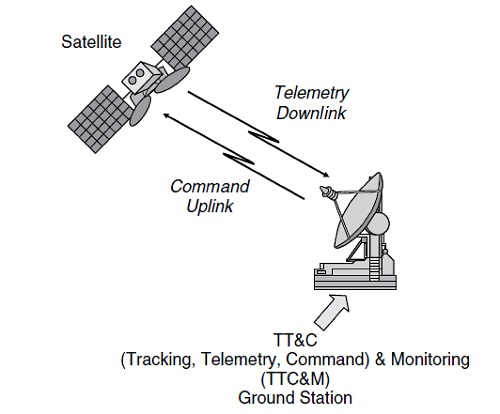
\includegraphics[width=0.5\paperwidth]{img/2/uplink_downlink.jpg}
    \caption{Satellite link uplink and downlink. Source: \cite{satcom_decription}}
    \label{intro:uplink_downlink}
\end{figure}

Depenending on the altitude of the orbit (fig. \ref{intro:orbits}), the distance between the satellite and the ground station varies - from Low Earth Orbit, with altitudes \SI{200}{\kilo\meter}~-~\SI{2000}{\kilo\meter}, via Geostationary Equatorial Orbit (\SI{35786}{\kilo\meter}) up to deep space communication ($2\cdot 10^{9}$~km for Voyager 1). Different types of orbit present much different difficulties - and completely different solutions are deployed on small CubeSats than large geostationary communication satellites. Depending on the orbit, the satellite can be visible only for short periods of time (as on LEO) or can be constanly monitored by the ground station (GEO). The main challenges the satellite link present are the large distance between the nodes, propagation and loss due to the atmosphere, but also limited resources on the satellite. The link consists of two nodes - the satellite and the ground station, with much different characteristics and design required. The satellite has limited dimensions and power available for the transmitter, different antenna pointing possibilities and the avaiable processing power is limited by the available space technology and power. On the other hand, the ground station can be built as large as needed, with high-gain antennas, power amplifier and high-sensitivity receivers to complement the limitations of the satellite. This chacaterises the link as highly assymetrical, with very high losses between the nodes and high processing gain on the ground station.
\begin{figure}
    \centering
    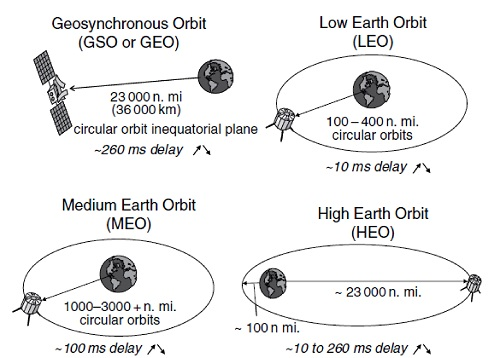
\includegraphics[width=0.5\paperwidth]{img/2/orbit_types.jpg}
    \caption{Different orbits and distances. Source: \cite{satcom_decription}}
    \label{intro:orbits}
\end{figure}

\section{Scope of the thesis}
The aim of this thesis was to design, verify, validate and deploy the communication system for second Polish satellite, PW-Sat2. The design covers all aspects of communication link design from the system point of view: the link design, space and ground segments and testing all the subsystems. Thesis should describe the choices and the practical design of the low-cost satellite link using both off-the-shelf hardware, custom designed components and Software Defined Radio, with custom digital signal processing. The designed system should provide a two-way data link between the operator and the satellite. Finally, the system was tested on the orbit, proving its parameters and reliability.

\chapter{PW-Sat2}
The presented system was designed specifically to be deployed onboard the PW-Sat2 satellite. PW-Sat2 is a student satellite project started in 2013 at Warsaw University of Technology by the Students Space Association members. Its main technical goal is to test new deorbit technology in the form of a large deorbit sail whereas the project purpose is to educate a group of new space engineers. PW-Sat2 is a 2-unit CubeSat satellite, designed for Low Earth Orbit. PW-Sat2 was launched on 3rd of December 2018 onboard SpaceX Falon 9 rocket. PW-Sat2 was placed on a sun-synchronous, polar, circular, \SI{590}{\kilo\meter}~-~orbit.
In the figure \ref{PW-Sat_render_01} an exploded render of PW-Sat2 is presented.
\begin{figure}[H]
    \centering
    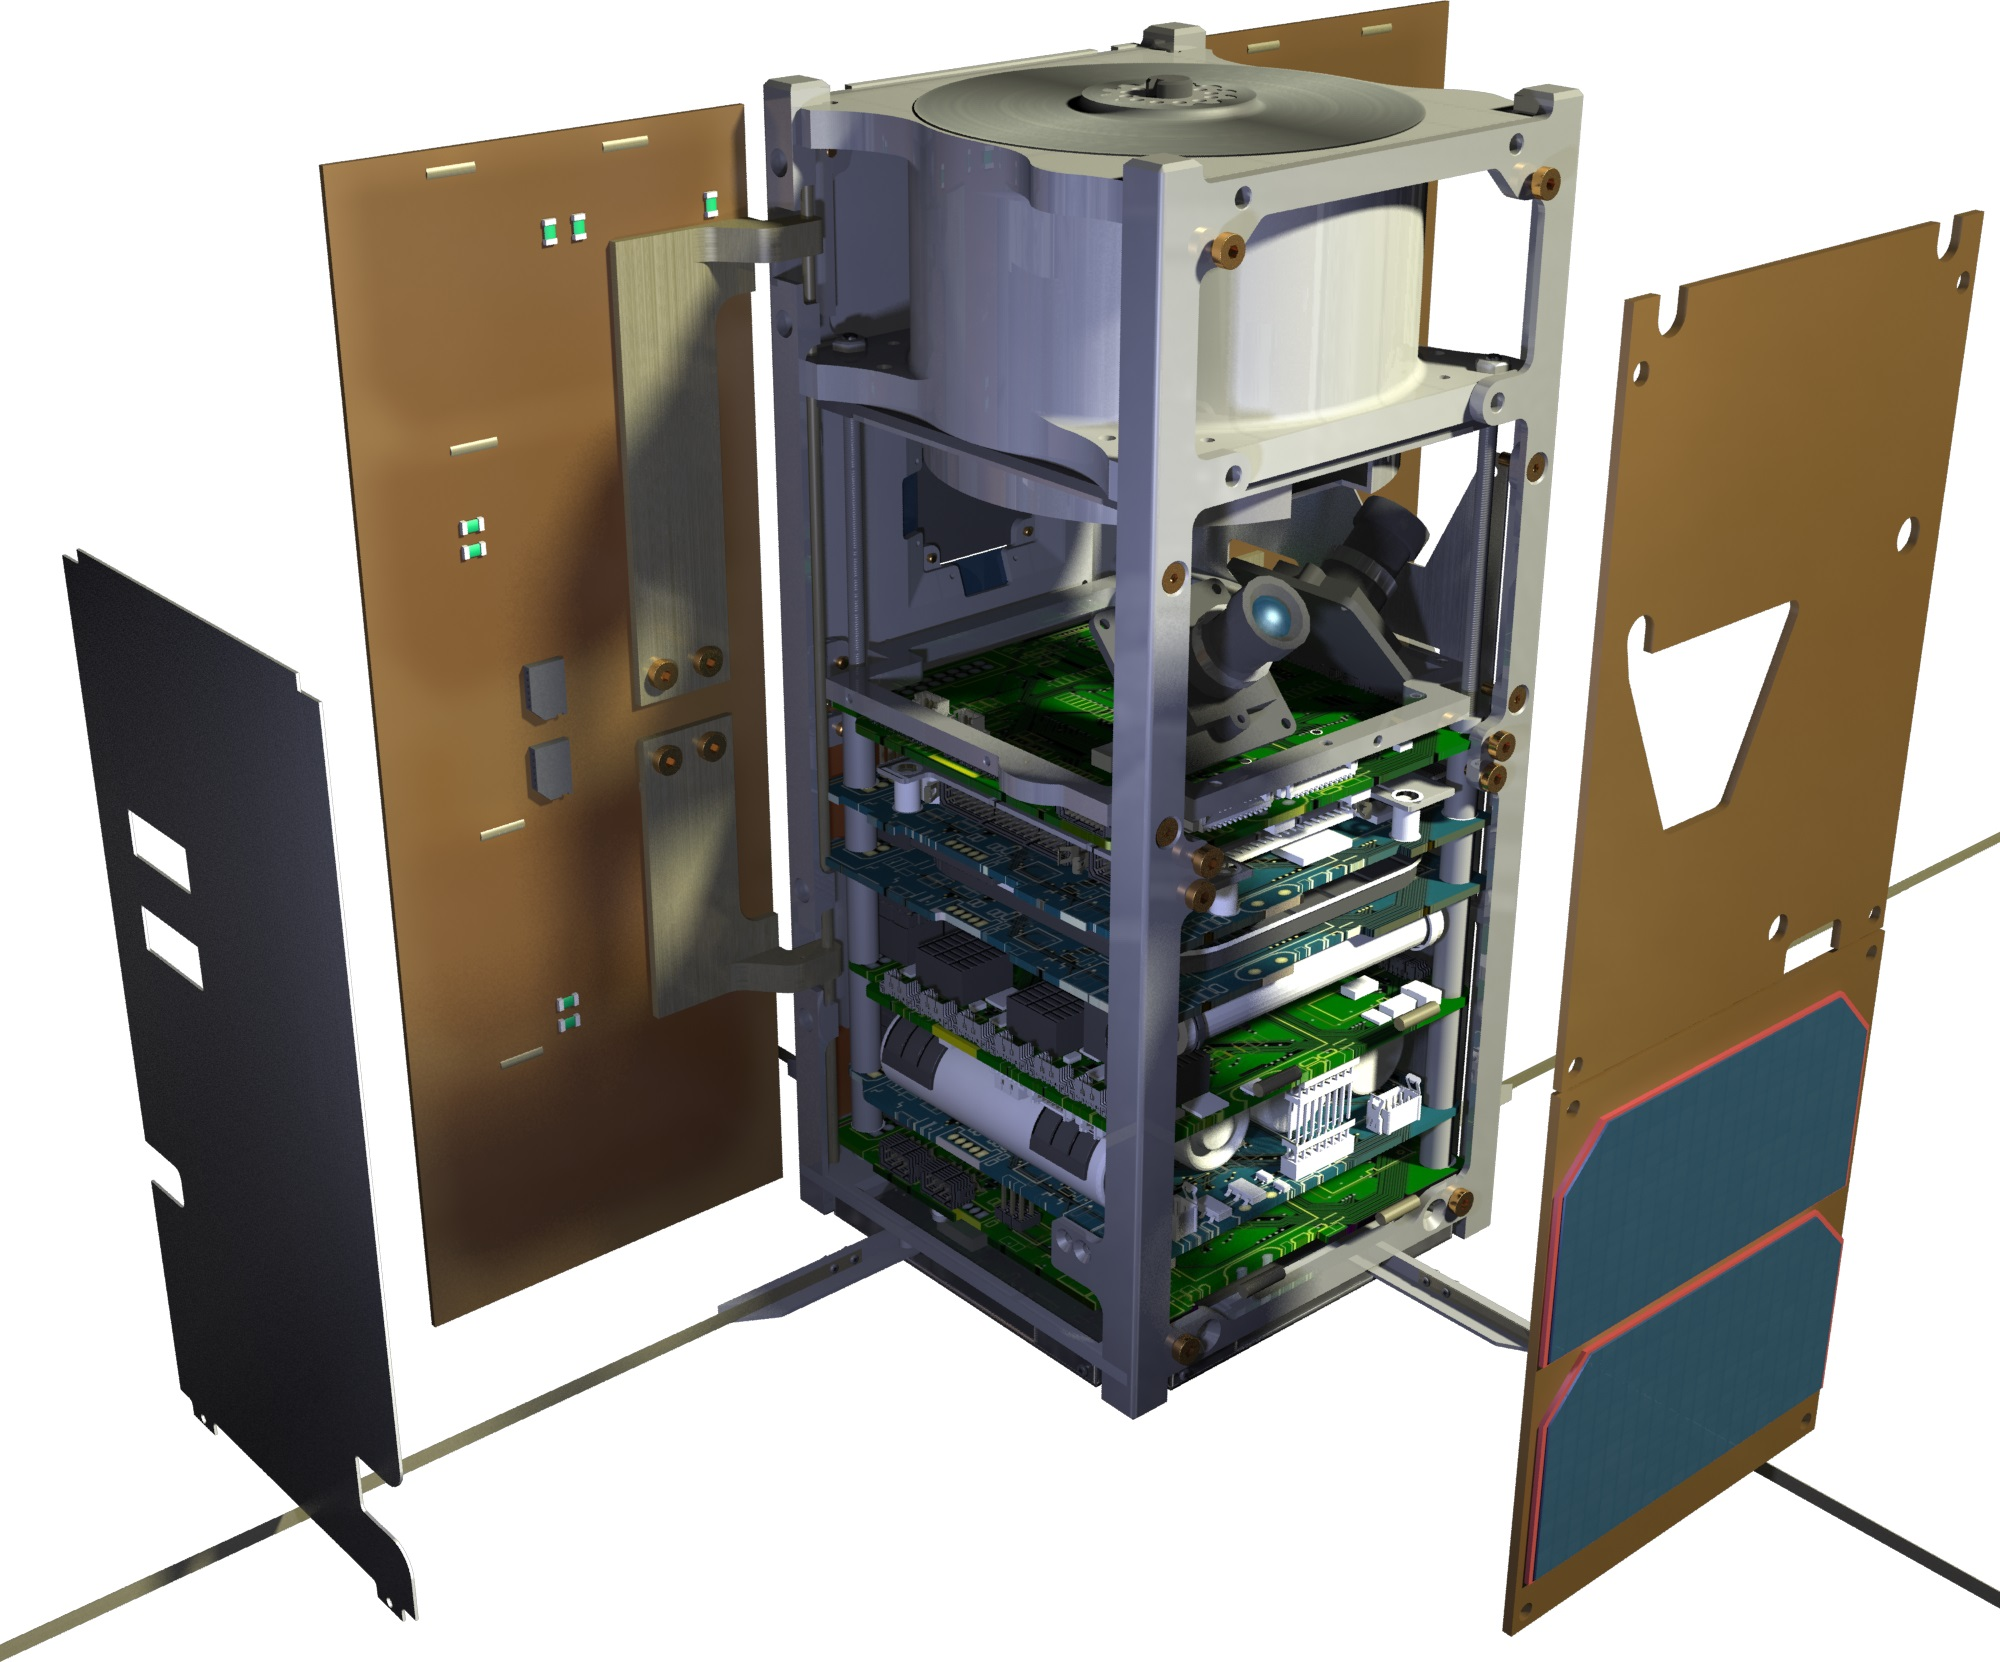
\includegraphics[width=0.65\paperwidth]{img/3/PW-Sat2_render_01.jpg}
    \caption{PW-Sat2 render. Source: \cite{PW_sat2_photo}}
    \label{PW-Sat_render_01}
\end{figure}

\section{CubeSat specification}
In 1999, California Polytechnic State University and Stanford University developed the CubeSat specifications to lower the barrier for developing and sending the satellite to the orbit of the Earth. Over 1000 CubeSats have been launched as of January 2019 (fig. \ref{nanosatellites_launched_by_years}). The CubeSat specification \cite{cubesat_spec} defines the CubeSat as a spacecraft built from number of "CubeSat units", with dimensions \si{10}x\si{10}x\SI{11.35}{\cm} and weight \SI{1.33}{\kilo\gram} each. Having defined requirements on the size, weight and deployment mechanism greatly reduces the cost of satellite launch, as no custom test specification, deployers and rocket parts have to be designed for each launch. CubeSats were designed to serve as an educational purpose for future engineers, to learn to design, build and deploy the Low Earth Orbit satellites. Currently, most of the CubeSats serve a commercial purpose, as a low-cost testbed for different experiments and subsystems.

\begin{figure}[h]
    \centering
    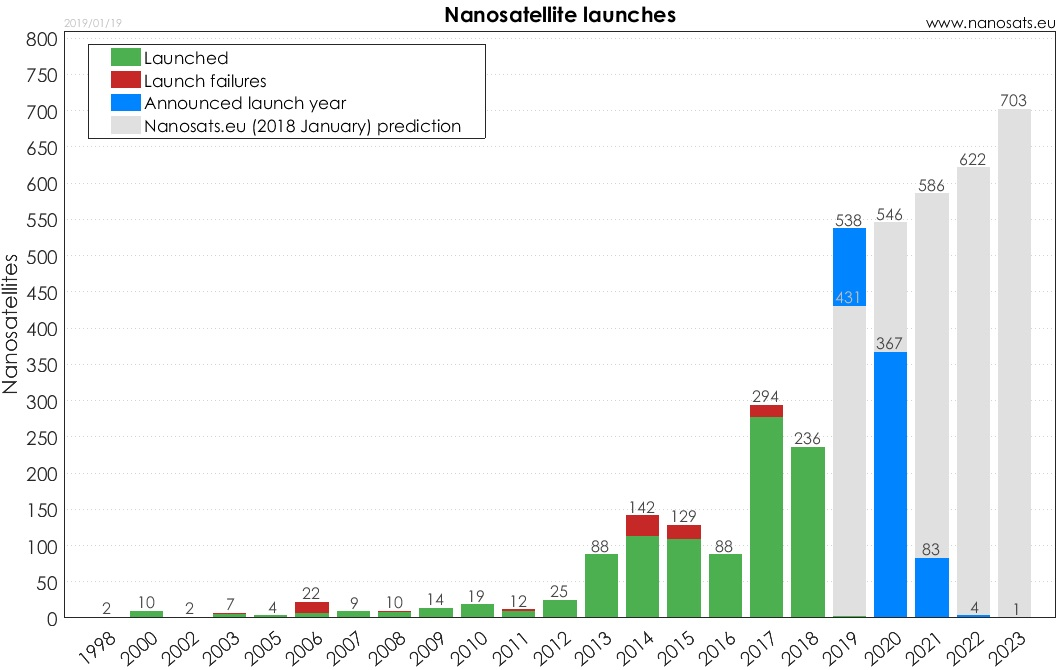
\includegraphics[width=0.65\paperwidth]{img/3/nanosatellites_launched_by_years.jpg}
    \caption{Nanosatellites launches. Source: \cite{nanosatellites_launched_by_years}}
    \label{nanosatellites_launched_by_years}
\end{figure}

\newpage

\section{Primary mission}
The primary mission of PW-Sat2 is to test the innovative deorbit technology - the deorbit sail. After satellite operations phase end, the deorbit sail opens and increases the atmospheric drag, shortening the satellite life time. A render of PW-Sat2 with an opened sail is presented in figure \ref{PW-Sat_render_sail}. As seen in the figure, the deorbit sail material is stretched on four flat springs, made of metal. The material of the sail is the \SI{5}{\micro\meter} mylar foil covered with aluminum. The sail is placed very close to the antennas - therefore, it can influence the antenna pattern and matching. 
\begin{figure}[h]
    \centering
    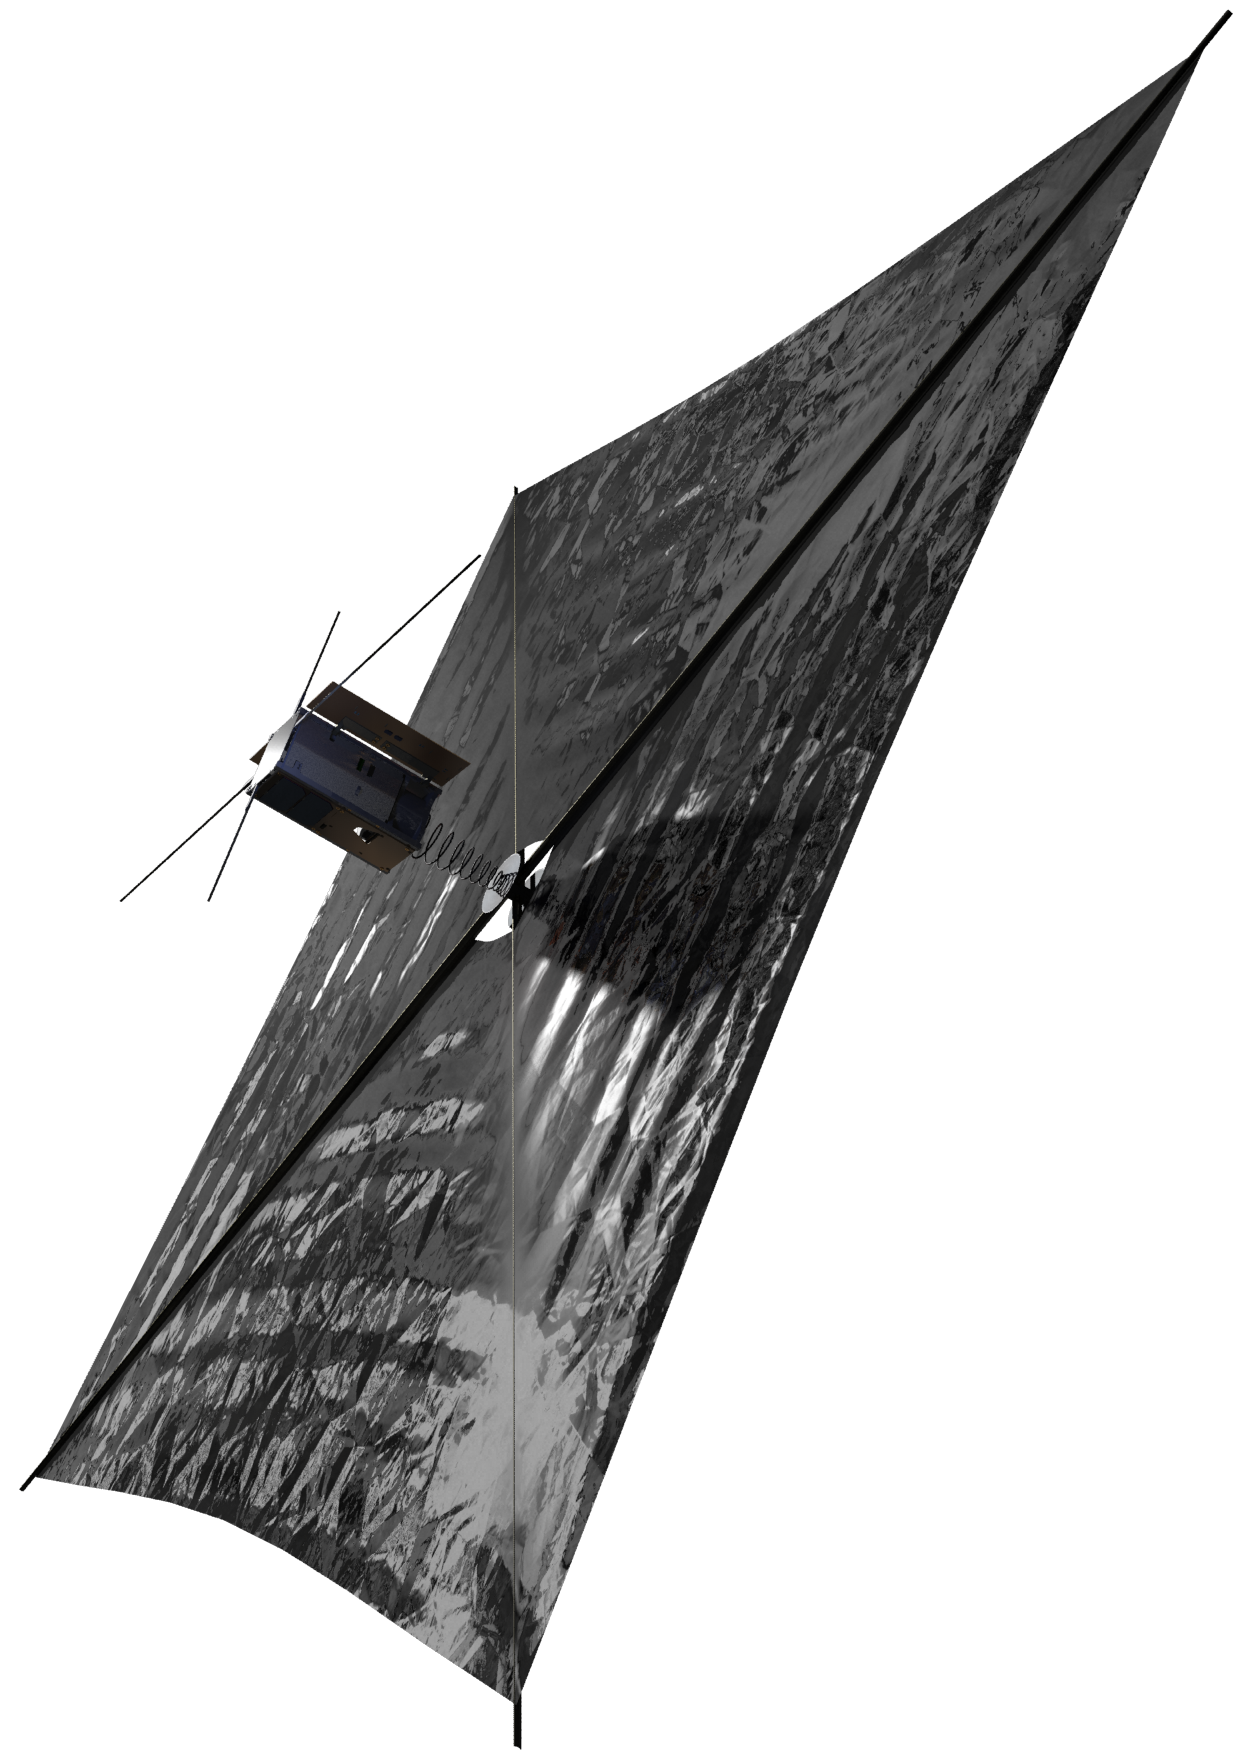
\includegraphics[width=0.38\paperwidth]{img/3/PW-Sat2_render_02.png}
    \caption{PW-Sat2 with opened sail and antennas. Source: \cite{PW_sat2_photo}}
    \label{PW-Sat_render_sail}
\end{figure}


\section{Secondary mission goals}
PW-Sat2 also have three secondary experiments, executed by the command from the operators on the ground. Those experiments will be ran when the link and power budget will allow. Secondary experiments include:
\begin{itemize}
    \item RadFET - ionizing radiation sensor, which measures threshold voltages on P-MOS transistors to estimate the TID absorbed by the satellite.
    \item Sun Sensor -  provides orientation between the satellite axes and the Sun, experimental sensor is compared with the commercial system readings. During the experiment, \si{12} Ambient Light Sensors provides information about their illumination, allowing the software to calculate angles to the Sun.
    \item Cameras - two VGA-resolution (\si{640}x\si{480}~px) onboard cameras with small and non-complicated optics which allow observing some parts of the deorbitation sail during its opening, monitor the sail condition during deorbitation phase and to take photos of the Earth.
\end{itemize}


\section{Solar array deployment}
PW-Sat2 have two deployable solar panels which are opened by the command from the On-Board Computer on the request of the satellite operator from the ground. Solar panels are mounted on two opposite walls. After opening, they create one large panel as seen on the figure \ref{PW-Sat_solar_panels}. The wings, on which solar panels are mounted, are made from aluminum; therefore, their deployment can change the antennas parameters as well.
\begin{figure}[h]
    \centering
    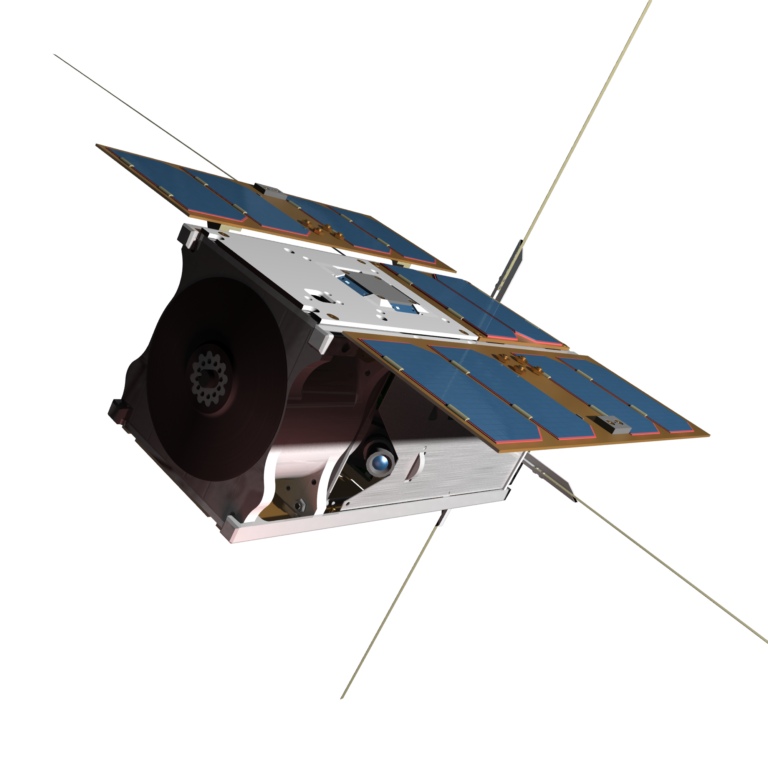
\includegraphics[width=0.45\paperwidth]{img/3/pwsat_solar_panels.png}
    \caption{PW-Sat2 with opened solar panels. Source: \cite{PW_sat2_photo}}
    \label{PW-Sat_solar_panels}
\end{figure}

\section{Attitude Determination and Control Subsystem}
Attitude Determination and Control Subsystem (ADCS) is responsible for controlling the satellite orientation. Random tumbling of the satellite after the deployment is caused by the asymmetric deployment forces and bumping with other CubeSats. To reduce rotational rate, PW-Sat2 use magnetic control of the orientation with magnetorquers, special type of an electromagnet, designed to interact with Earths' magnetic field. The subsystem controls the currents of the magnetorquers. For PW-Sat2, the only implemented ADCS mode is detumbling - the algorithm used to reduce the random tumbling to a very low rotational rate (in the order of degrees/second). Therefore, the very slow random tumbling of the satellite is assumed, which forces to use omnidirectional antennas, as the pointing is not possible.

\section{Electrical Power System}
Electrical Power System is responsible for power conversion from the solar panels, energy storage in the onboard battery and power distribution to the other subsystems. Electrical power is generated with \si{12} space qualified triple-junction solar cells, resulting in total average power of \SI{1}{\watt} (assuming random tumbling). The Electrical Power System harvests this energy and distribute it to the other subsystems, as shown in figure \ref{pwsat_eps_distribution}. During the mission, the average available power from the solar panels were estimated at \SI{1.5}{\watt} before sail deployment and \SI{0.75}{\watt} after the sail deployment (the sail covers around half of the sphere). The total average power for the communication system was presumed to \SI{0.6}{\watt} average, with peak current consumption of \SI{5}{\watt} during transmission.
\begin{figure}
    \centering
    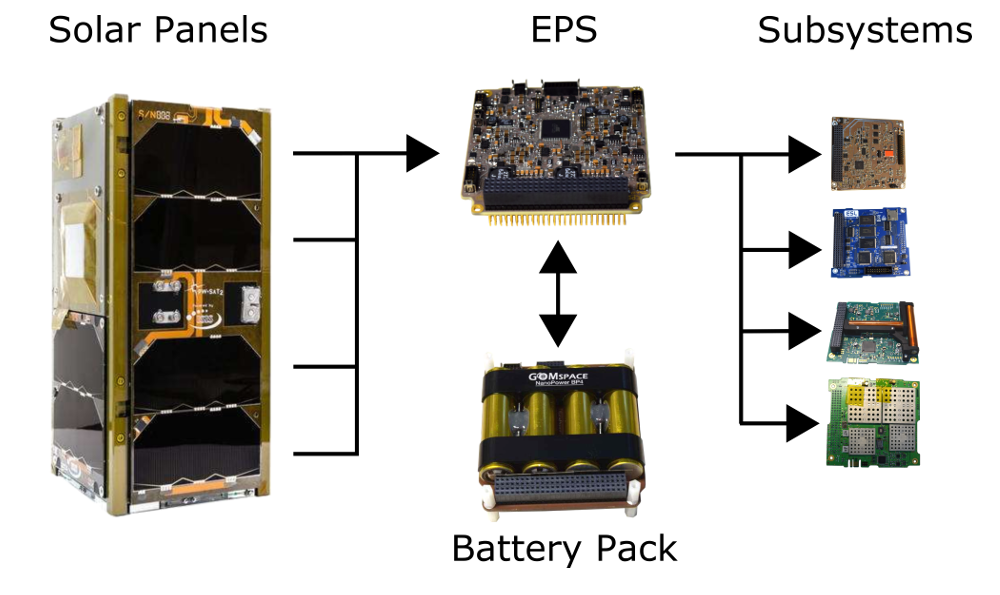
\includegraphics[width=0.7\paperwidth]{img/3/pwsat_eps_distribution.png}
    \caption{PW-Sat2 energy distribution. Source: \cite{PW_sat2_photo}}
    \label{pwsat_eps_distribution}
\end{figure}

\section{Mission plan and system lifetime}
\label{sect:mission_phases}.
The PW-Sat2 mission is divided into two main phases:
\begin{itemize}
    \item Normal phase - planned to take up to 40 days, before the opening of the deorbit sail. The satellite should perform secondary mission goals during this phase, by the telecommands from operators on the ground. 
    \item Extended phase - activities after the sail deployment. In this phase half of the energy is available for the subsystems. The sail condition and satellite status should be monitored by the operations team up to the moment of satellite deorbitation, by telemetries and photos. Extended phase can take up to about \si{2}~years.
\end{itemize}

\chapter{Radio communication with the nanosatellites - state of the art}

\section{Frequency allocation}
For non-commercial, radio amateur CubeSats
% The most common radio bands used in CubeSat designs are VHF, UHF and S-band. S-band is usually used when high data rate (~\SI{10}{\Mbps}) are necessary. Typical designs for low-rate data link are full-duplex combo or simplex VHF/UHF radio.

% PW-Sat1 \cite{pwsat1_website_ska} used full-duplex VHF-downlink and UHF-uplink radio. During its mission, operation team was reporting uplink stability issues, which was caused by very low Signal to Noise ratio on the satellite. The design team narrowed down the issue to very high level of interference in the UHF band on the orbit, which probably is caused by the high power signal sources on the ground, such as radars.

% The selected bands for PW-Sat2 operation were either simplex VHF or full-duplex: VHF-up, UHF-down.


\section{Subsystem review}
There are number of commercially available solutions and subsystems. Usually they are divided into subsystems, allowing user to mix different suppliers depending on the requirements, assuring they are compatible.

\subsection{Cubesat commmunication diagram}
Typical Low Earth Orbit satellite communication systems is shown in the figure \ref{comm_diagram}.

\begin{figure}
    \centering
    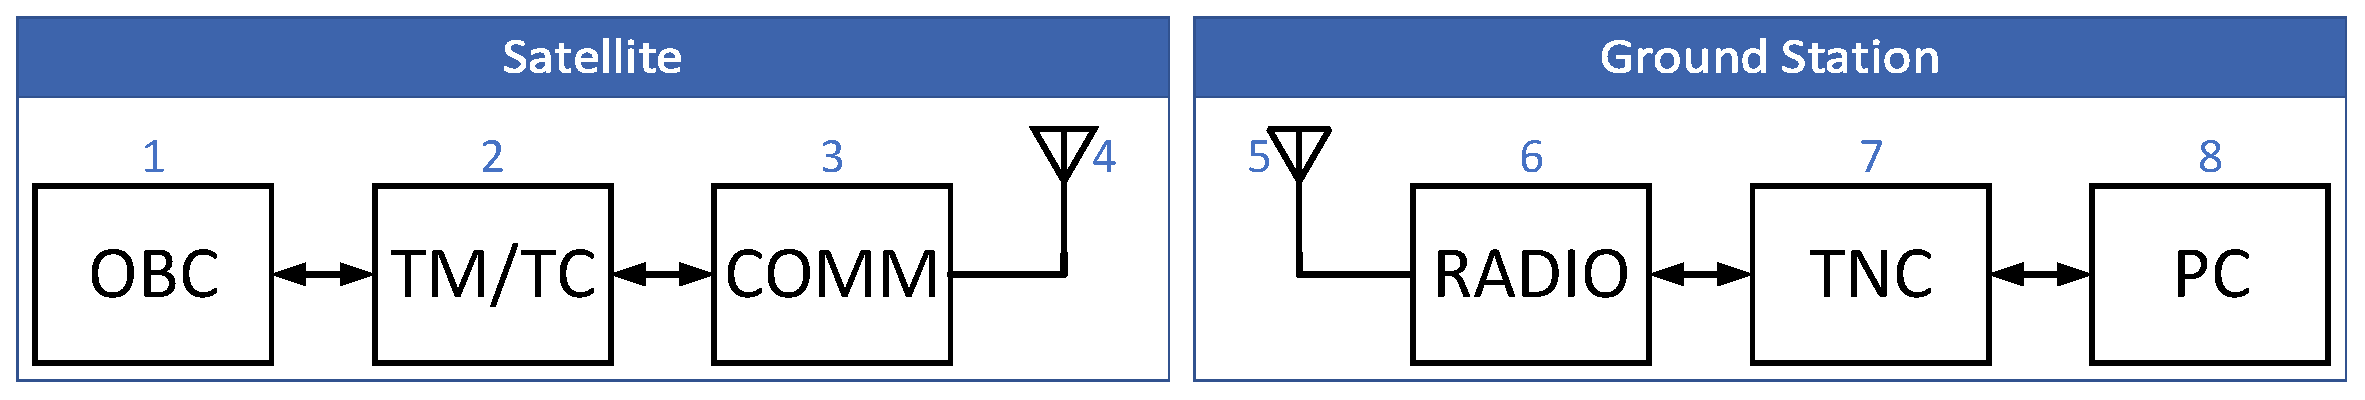
\includegraphics[width=0.7\paperwidth]{img/4/comm_diagram.eps}
    \caption{General communication system diagram}
    \label{comm_diagram}
\end{figure}

It consists of:
\begin{enumerate}
    \item On-Board Computer - controls the satellite, generates data and receives telecommands,
    \item Telemetry/Telecommand generator - translates between packets and baseband signal (modulator and demodulator),
    \item COMM - communications module, performs up/down conversion, amplification and antenna matching, usually on smaller missions it is integrated with TMTC on one module,
    \item Satellite antenna(s), typically omnidirectional to provide coverage during random satellite tumbling
    \item Ground station antenna(s), directional to maximize gain of the radio link,
    \item RADIO - radio system, typically a low noise amplifier with up/down converter and modulator, converts radio frequencies to baseband signals,
    \item Terimnal Network Controller - translates between packets and baseband signal, can be done as a separate device or in software in the PC,
    \item PC - a computer, which operator of the satellite uses to generate and receive data packets.
\end{enumerate}

\subsection{Cubesat antennas}
Cubesat dimensions are strict and defined in the CubeSat Design Specification \cite{cubesat_spec} as \si{100}x\si{100}~mm square \ref{CubeSat_max_dim}. This poses a requirement of antenna unfolding for antennas larger than side width. Usually this is required for all sub-GHz band, such as considered VHF and UHF bands. Higher bands, such an S-band, usually use patch antennas mounted on the wall.

\begin{figure}
    \centering
    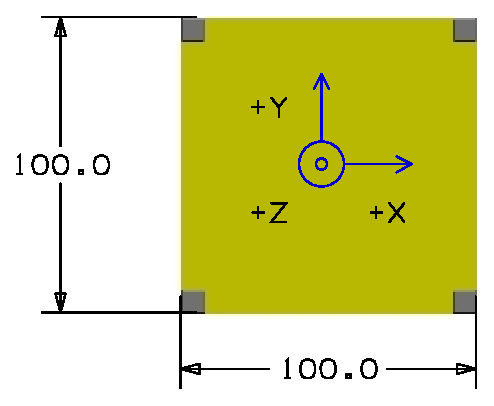
\includegraphics[width=0.5\paperwidth]{img/4/cubesat_dimensions.eps}
    \caption{CubeSat maximum dimensions, top view. Source \cite{cubesat_spec}.}.
    \label{CubeSat_max_dim}
\end{figure}

Antennas are usually unfolded by the spring action of the antennas itself and they are released by the on-board computer (by the thermal knife). Three typical antenna deployment systems are shown in the figures \ref{stiff_antenna_pic}, \ref{m_cubed}, \ref{isis_dipole_antenna}.

Typical unidirectional VHF/UHF antennas are dipoles, monopoles or turnstille. Selecting one depends on the mission requirements and link budget. Turnstille antenna, providing best link budget and circular polarization require that radiation elements are mounted on two sides of the CubeSat. Dipole option uses two elements is not as dependent on the ground reference (main structure) as the monopole antenna.

\begin{figure}
    \centering
    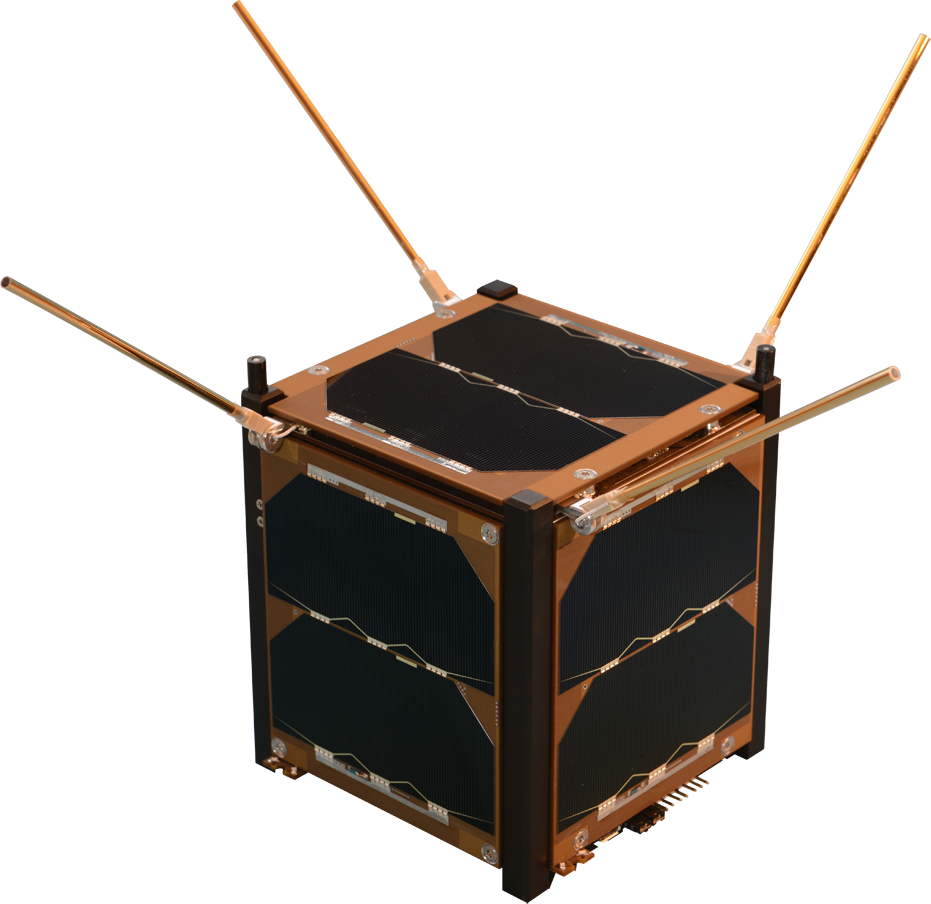
\includegraphics[width=0.5\paperwidth]{img/4/antenna_stiff.png}
    \caption{Deployed stiff antenna. In the stowed configuration they are along the solar panels. Source \cite{stiff_antenna_paper}.}.
    \label{stiff_antenna_pic}
\end{figure}

\begin{figure}
    \centering
    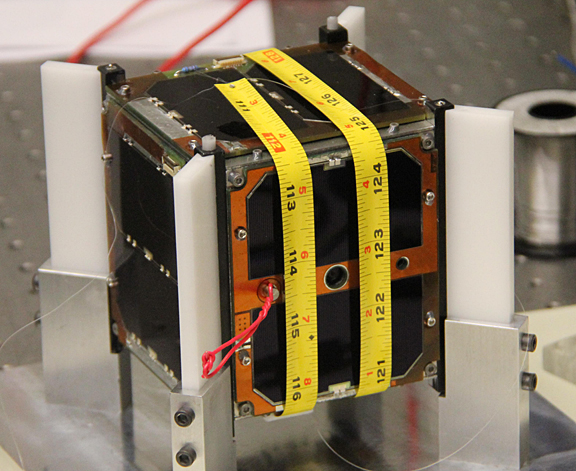
\includegraphics[width=0.5\paperwidth]{img/4/m-cubed.jpg}
    \caption{Tape measure antenna in the stowed configuration. Flat spring action forces antenna to deploy itself after its release. Source \cite{m_cubed}.}.
    \label{m_cubed}
\end{figure}

\begin{figure}
    \centering
    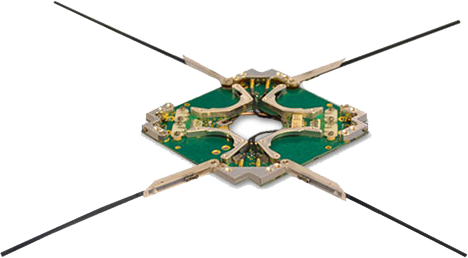
\includegraphics[width=0.5\paperwidth]{img/4/isis_dipole.png}
    \caption{Flat spring antennas rolled inside the CubeSat square. Released by the thermal knife burning the lock of the antenna doors. Source \cite{isis_dipole_antenna}.}.
    \label{isis_dipole_antenna}
\end{figure}

\subsection{Ground station antennas}
Space communication antennas require very large gain due to the distance between the stations and the omnidirectivity of the CubeSat antennas. Transmit power of the satellite is usually rather low (\SI{1}{\watt} or less).

Most of the designs use Yagi-Uda antennas, in circular polarization (cross-yagi with phasing). They are typically 9-11 elements long for VHF and 17-19 elements for UHF. Yagi-Uda antennas can be also phased as an array of antennas (1x2, 2x2 configuration etc.) improving gain and directivity. This however requires the antenna mast to withstand the size and weight of the system. Required power gain is dependent on the mission itself and the reliability of the link. Random tumbling and CubeSat antennas with dips in the radiation pattern (as monopole and dipole) require more directivity and power gain than attitude-controlled satellites. Direcitivity of the antenna also affects antenna noise temperature.

Depending on the mission, one, two or more antennas can be required due to the number of bands used. 

Due to the directivity of the antennas, their half-power beam width is around \si{2}-\SI{10}{\degree}. Therefore another required element of the ground station is the antenna rotator, which has to support the required weight, size and the location of the ground station.

In the figure \ref{isis_gs} the commercially available ISIS VHF/UHF ground station is shown, which employs two cross-yagi antennas (VHF, UHF), antenna mast and rotator and rotator controller.

\begin{figure}
    \centering
    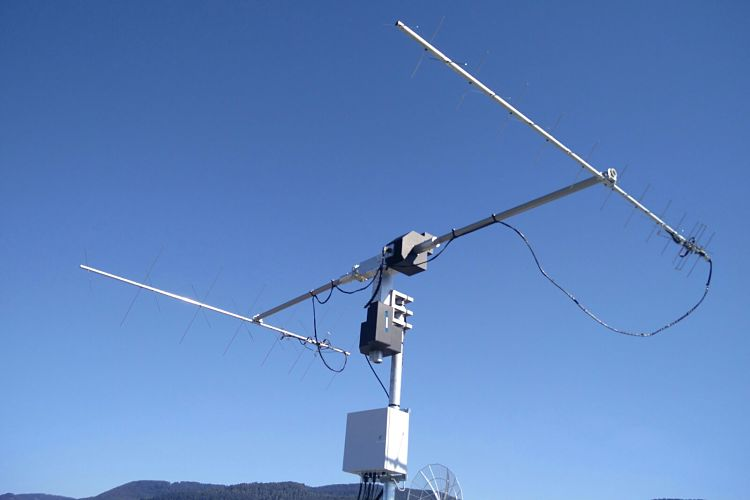
\includegraphics[width=0.5\paperwidth]{img/4/isis_gs.jpg}
    \caption{ISIS Ground Station. Source \cite{isis_gs}.}.
    \label{isis_gs}
\end{figure}

\subsection{Satellite communication subsystem}
Communication subsystem of the satellite is responsible of transmitting and receiving radio signals, modulating/demodulating them and providing data link for the On Board Computer. It has to be compatible with selected mechanical configuration, available data interfaces and the antennas to be installed. Most of the designs use custom design radio systems, using heterodyne receivers/transmitters (Fig. \ref{clyde_comm}), however there are an Software-Defined Radio systems, such as Gomspace SDR Platform \ref{gomspace_comm}.

\begin{minipage}{\linewidth}
    \centering
    \begin{minipage}{0.45\linewidth}
        \begin{figure}[H]
            \centering
            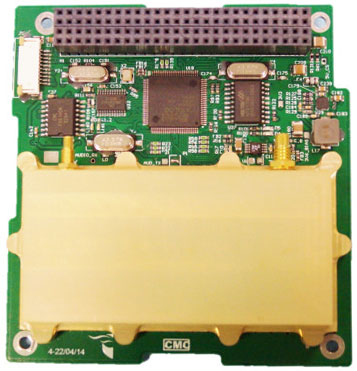
\includegraphics[width=0.32\paperwidth]{img/4/clyde_comm.jpg}
            \caption{CPUT UTRX from Clyde Space. Source: \cite{clyde_comm}}
            \label{clyde_comm}
        \end{figure}
    \end{minipage}
    \hspace{0.05\linewidth}
    \begin{minipage}{0.45\linewidth}
        \begin{figure}[H]
            \centering
            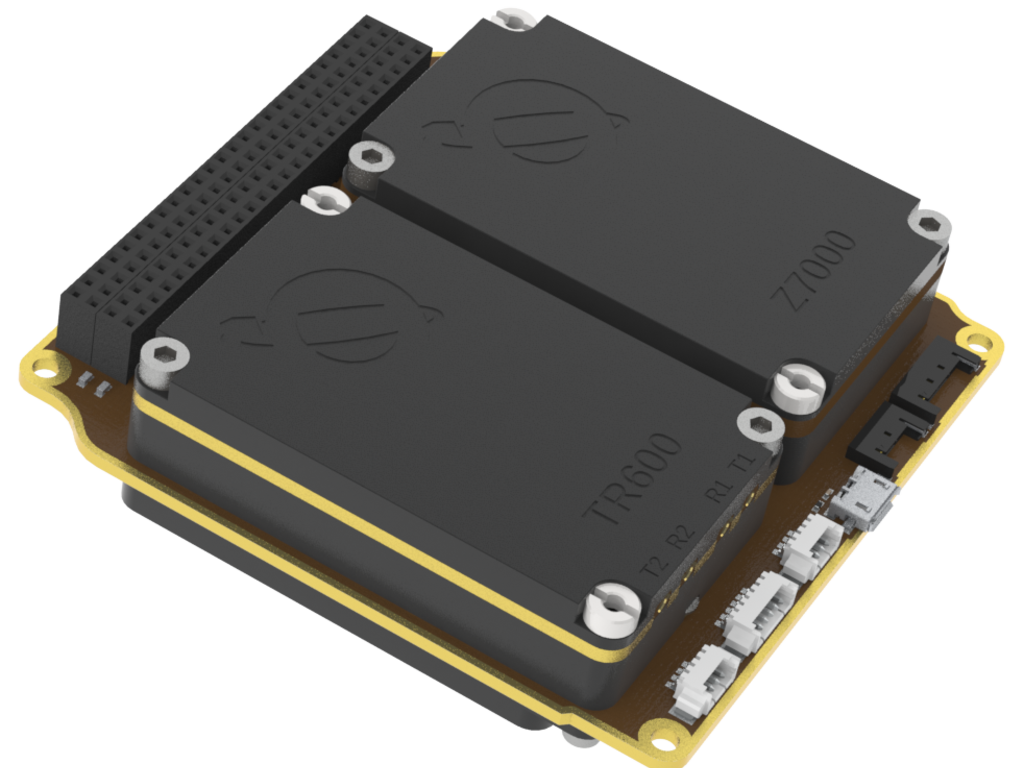
\includegraphics[width=0.35\paperwidth]{img/4/gomspace_sdr.png}
            \caption{Space qualified Software Defined Radio (SDR) Platform. Source: \cite{gomspace_comm}}
            \label{gomspace_comm}
        \end{figure}
    \end{minipage}
\end{minipage}


\subsection{Ground segment communication subsystem}
\subsubsection{Transmitter}
Due to the typically lower sensitivity and omnidirectional antenna on the satellite the uplink EIRP has to be very large, requiring not only directional antennas but also high output power (\si{100}-\SI{1500}{\watt}).
Depending on the modulation required, relatively cheap radio amateur transceivers can be used to modulate and amplify transmit signals, such as ICOM 910H or KENWOOD TS-2000 E (Fig. \ref{kenwood_ts2000}). As those types of radios were designed to transmit speech (bandwidth up to about \SI{10}{\kHz}) they can be used only to transmit signals which are FM, AM or SSB modulated. For other modulation and/or bandwidth the radio signal has to be generated by other type of radio (integrated or software-defined) and power amplifier.

Depending on the required output power, high-power amplifier can be used to further increase output power up to several kilo-watts. 

\begin{minipage}{\linewidth}
    \centering
    \begin{minipage}{0.45\linewidth}
        \begin{figure}[H]
            \centering
            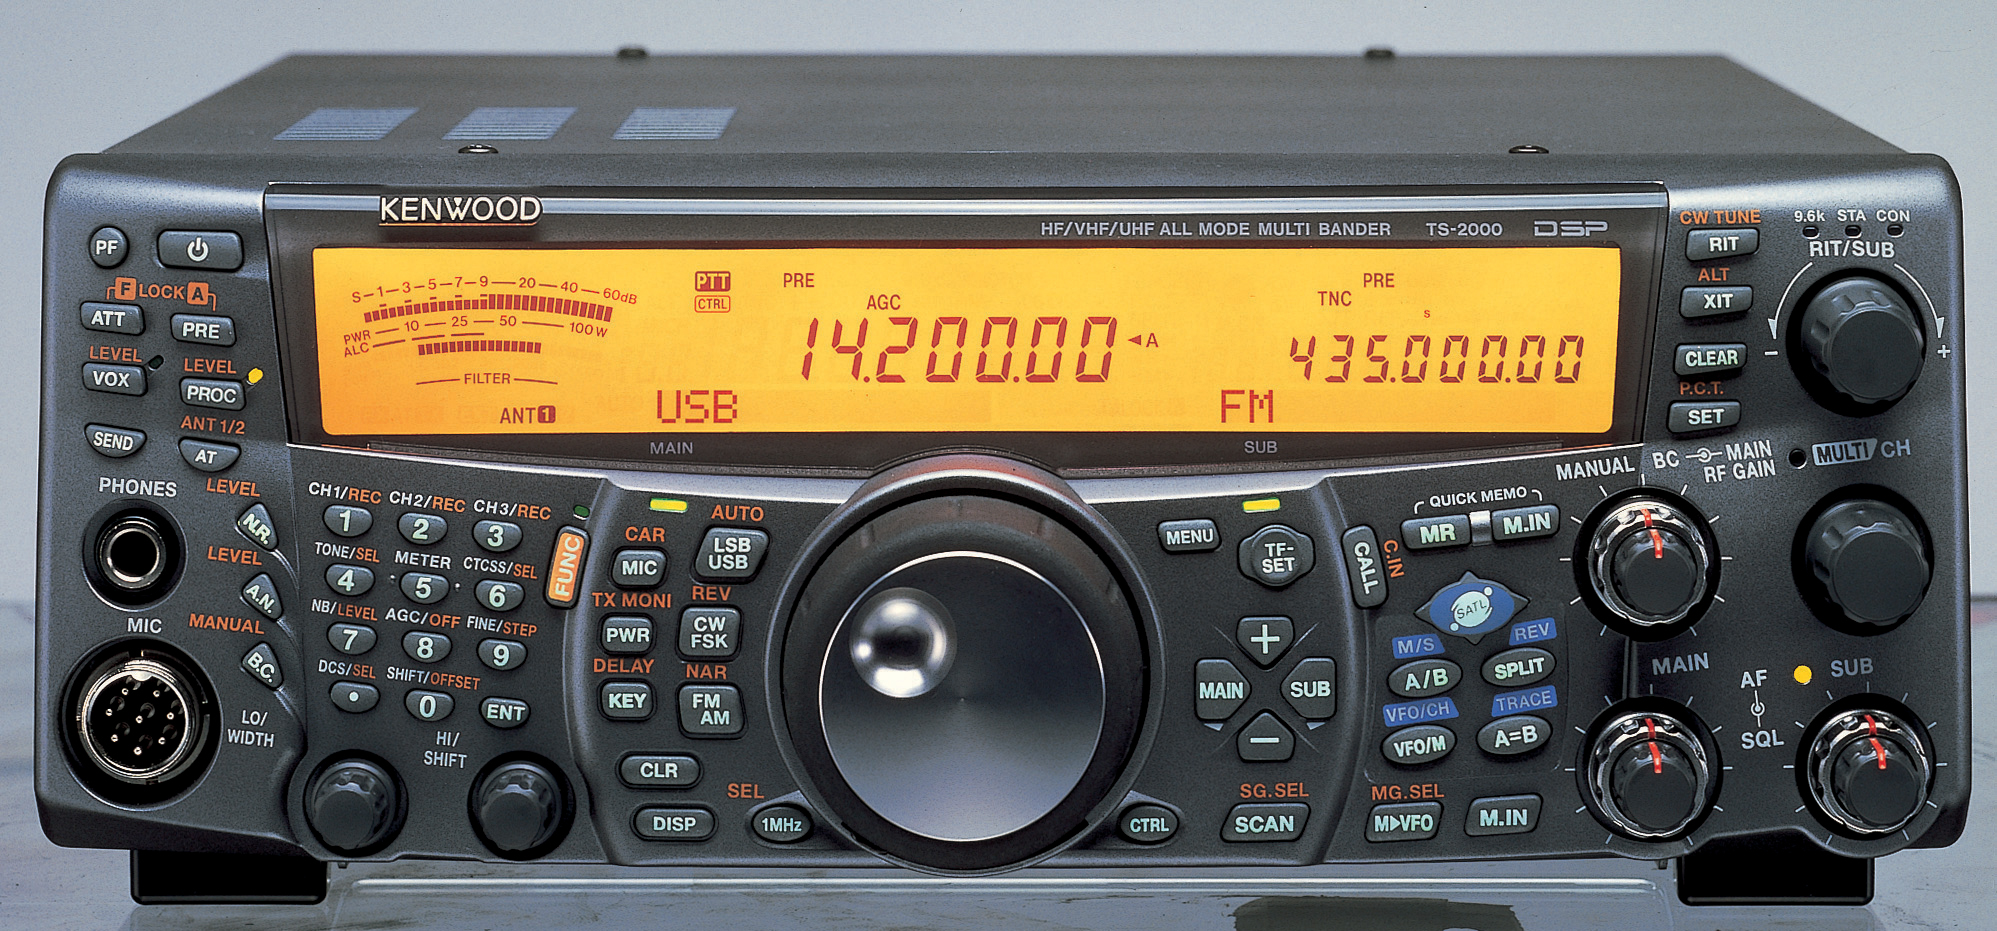
\includegraphics[width=0.35\paperwidth]{img/4/kenwood_ts2000.jpg}
            \caption{KENWOOD TS-2000 E all mode transceiver. Source: \cite{kenwood_ts2000}}
            \label{kenwood_ts2000}
        \end{figure}
    \end{minipage}
    \hspace{0.05\linewidth}
    \begin{minipage}{0.45\linewidth}
        \begin{figure}[H]
            \centering
            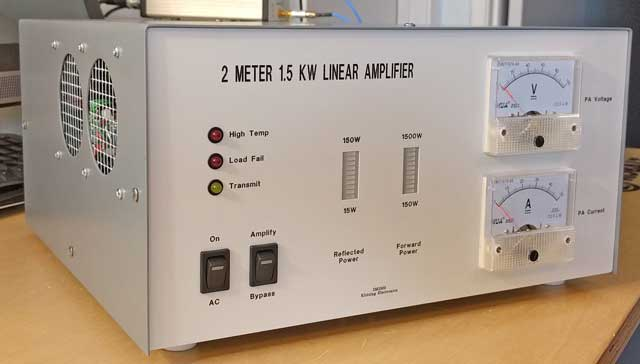
\includegraphics[width=0.35\paperwidth]{img/4/vhf_1500w_pa.jpg}
            \caption{\SI{1500}{\watt} VHF power amplifier. Source: \cite{vhf_1500w_pa}}
            \label{vhf_1500w_pa}
        \end{figure}
    \end{minipage}
\end{minipage}

\subsubsection{Receiver}
The receiver on the ground has to complement the space segment. Due to relatively low transmit power on the satellite, the receiver sensitivity should be very high. Additionally, receiver intermodulation performance should withstand possible blocking signals which are present on the ground.

To increase the sensitivity, Low Noise Amplifier has to be installed close to the antenna, such as LNA SSB-70 for UHF band (Fig. \ref{ssb_lna70}), which has Noise Figure of about \SI{0.35}{\dB}. Intermodulation and blocking is provided at the first stage by placing low-loss filter before the LNA, such as Cavity filters (Fig. \ref{cavity_uhf}).

\begin{minipage}{\linewidth}
    \centering
    \begin{minipage}{0.45\linewidth}
        \begin{figure}[H]
            \centering
            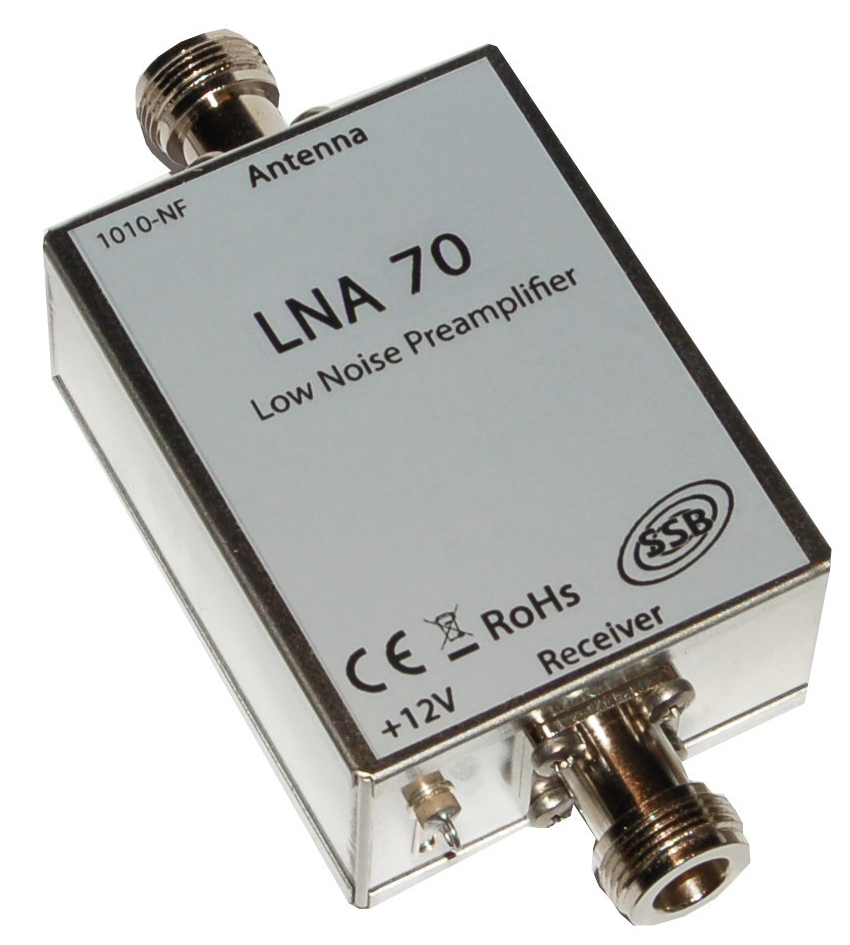
\includegraphics[width=0.3\paperwidth]{img/4/ssb_lna70.jpg}
            \caption{LNA SSB-70 Low Noise Amplifier for UHF band. Source: \cite{ssb_lna70}}
            \label{ssb_lna70}
        \end{figure}
    \end{minipage}
    \hspace{0.05\linewidth}
    \begin{minipage}{0.45\linewidth}
        \begin{figure}[H]
            \centering
            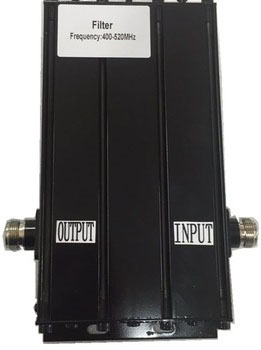
\includegraphics[width=0.3\paperwidth]{img/4/cavity_uhf.jpg}
            \caption{LBQ-450 3-cavity UHF bandpass filter. Source: \cite{cavity_uhf}}
            \label{cavity_uhf}
        \end{figure}
    \end{minipage}
\end{minipage}


Radio signal, pre-amplified by the low-noise amplifier is down-converted to the baseband and de-modulated. This can be performed by the integrated radio transceiver (same as the transmitter, this emposes the same modulation constraints as for the transmitter) or by the software-defined radio, such as an NI-USRP 2901 (Fig. \ref{ni_2901}) or FUNcube Dongle Pro+ (which was specifically designed for the FUNcube CubeSat - Fig. \ref{funcube}).

\begin{minipage}{\linewidth}
    \centering
    \begin{minipage}{0.45\linewidth}
        \begin{figure}[H]
            \centering
            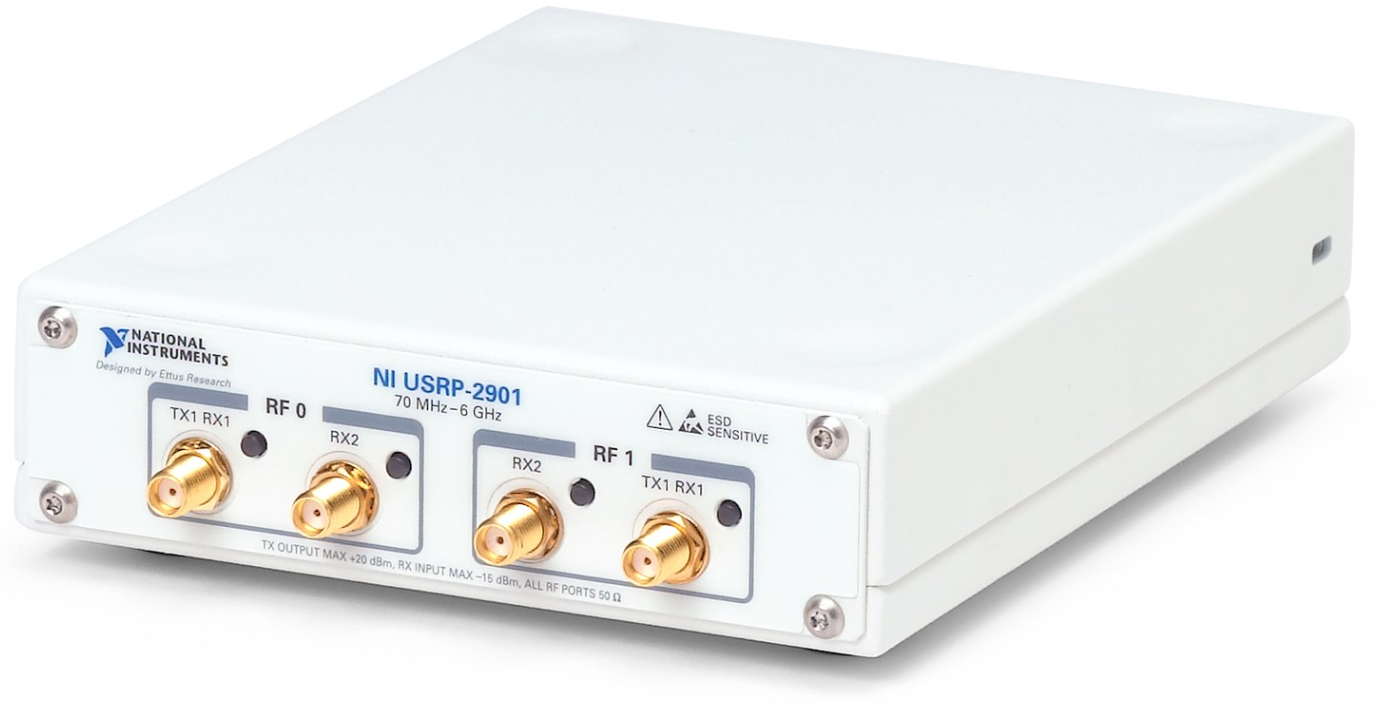
\includegraphics[width=0.3\paperwidth]{img/4/ni_2901.png}
            \caption{USRP-2901 Software Defined Radio Device. Source: \cite{ni_2901}}
            \label{ni_2901}
        \end{figure}
    \end{minipage}
    \hspace{0.05\linewidth}
    \begin{minipage}{0.45\linewidth}
        \begin{figure}[H]
            \centering
            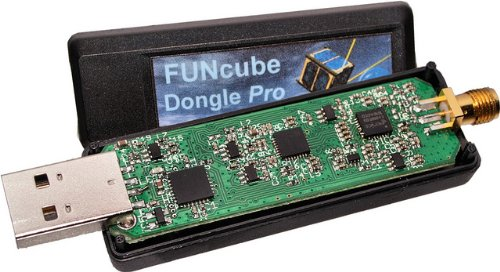
\includegraphics[width=0.3\paperwidth]{img/4/funcube.jpg}
            \caption{FUNcube Dongle Pro+. Source: \cite{funcube}}
            \label{funcube}
        \end{figure}
    \end{minipage}
\end{minipage}

After down-conversion baseband signal has to be de-modulated, which is done by the Terminal Network Controller. This can be implemeneted as a custom hardware solution (analog-to-digital converter and custom digital signal processor, for example TNC-X shown in the figure \ref{tncx}) or by pure software. Software solution has more flexibility but require a PC to perform signal processing, as is the only option for software-defined radio. One of the available TNC software using audio card is the Direwolf \cite{direwolf}.

\begin{figure}
    \centering
    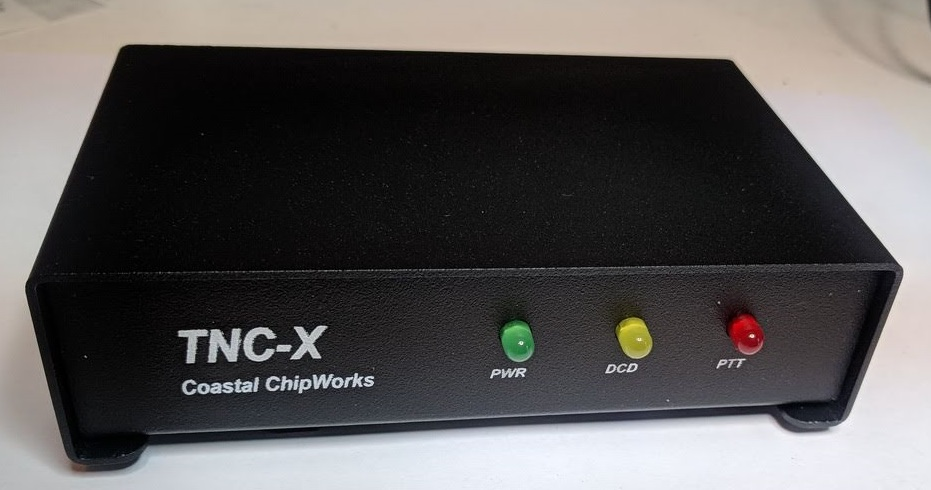
\includegraphics[width=0.3\paperwidth]{img/4/tncx.jpg}
    \caption{Terminal Network Controller TNC-X. Source: \cite{tncx}}
    \label{tncx}
\end{figure}



\section{Similar missions and designs}
In this section, three already flown satellite missions are described: PW-Sat, SwissCube and MOVE-I. 
\subsection{PW-Sat}
First polish satellite, PW-Sat, was launched in year \si{2012}. It was build on Warsaw Univeristy of Technology, with Space Research Centre PAS support. 

PW-Sat used ISIS TRXUV on-board communication module, with two (UHF uplink + VHF downlink) dipoles. Used modulations were AFSK \SI{1200}{\bps}. Radio transmit output power was \SI{30}{\dBm}. 
Ground station was built on Nicolaus Copernicus Astronomical Center in Warsaw, using \si{4}, \si{9}~element synphase cross-yagi VHF antennas for downlink and \si{4}, \si{19}~element synphase cross-yagi UHF antennas for uplink. Peak output power for uplink was \SI{100}{\watt} from the ICOM 910H transceiver.

PW-Sat and its ground station antennas are shown in the figures \ref{PW-Sat1_pic} and \ref{CAMK_pic}.

\begin{minipage}{\linewidth}
    \centering
    \begin{minipage}{0.45\linewidth}
        \begin{figure}[H]
            \centering
            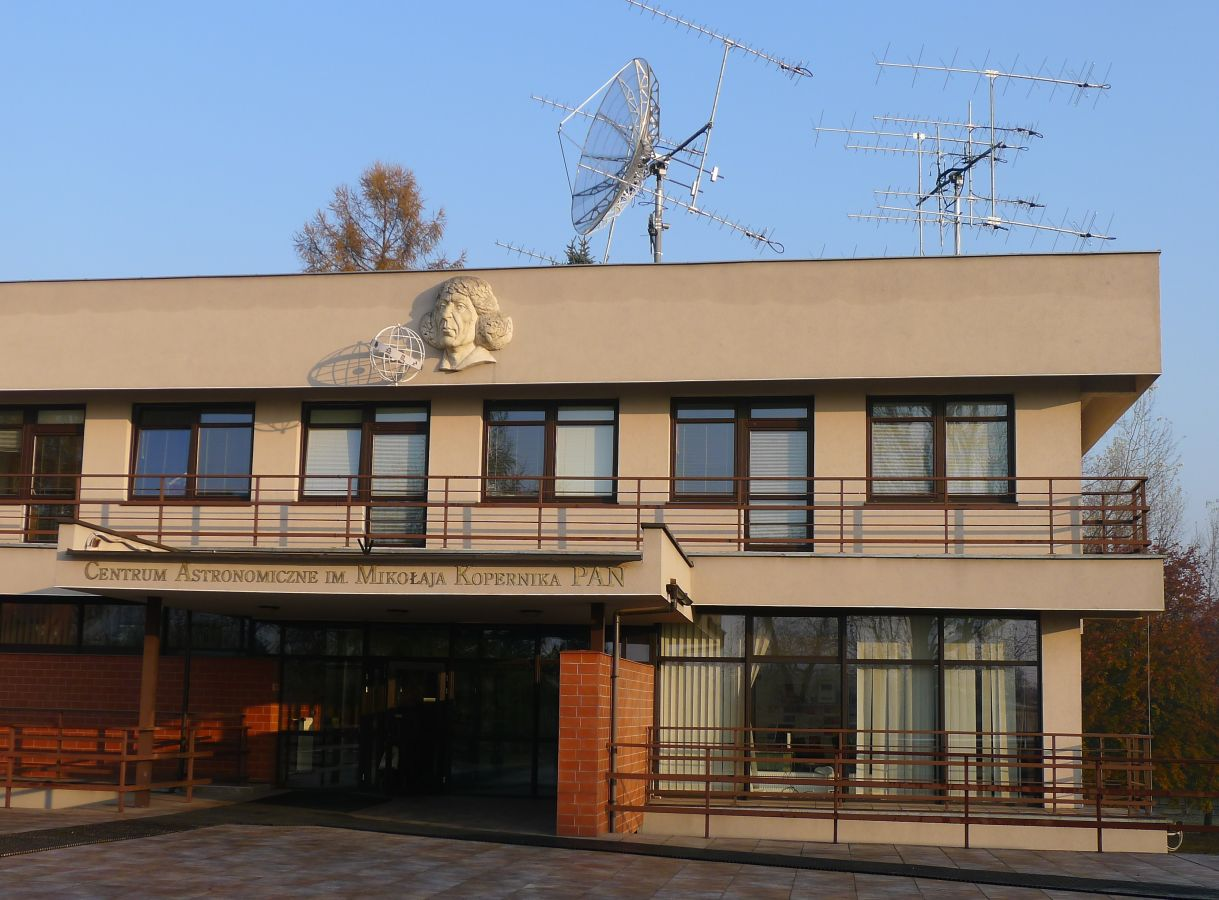
\includegraphics[width=0.32\paperwidth]{img/4/camk_pic.jpg}
            \caption{Nicolaus Copernicus Astronomical Center in Warsaw. PW-Sat antennas on the right. Source: \cite{camk_pic}}
            \label{CAMK_pic}
        \end{figure}
    \end{minipage}
    \hspace{0.05\linewidth}
    \begin{minipage}{0.45\linewidth}
        \begin{figure}[H]
            \centering
            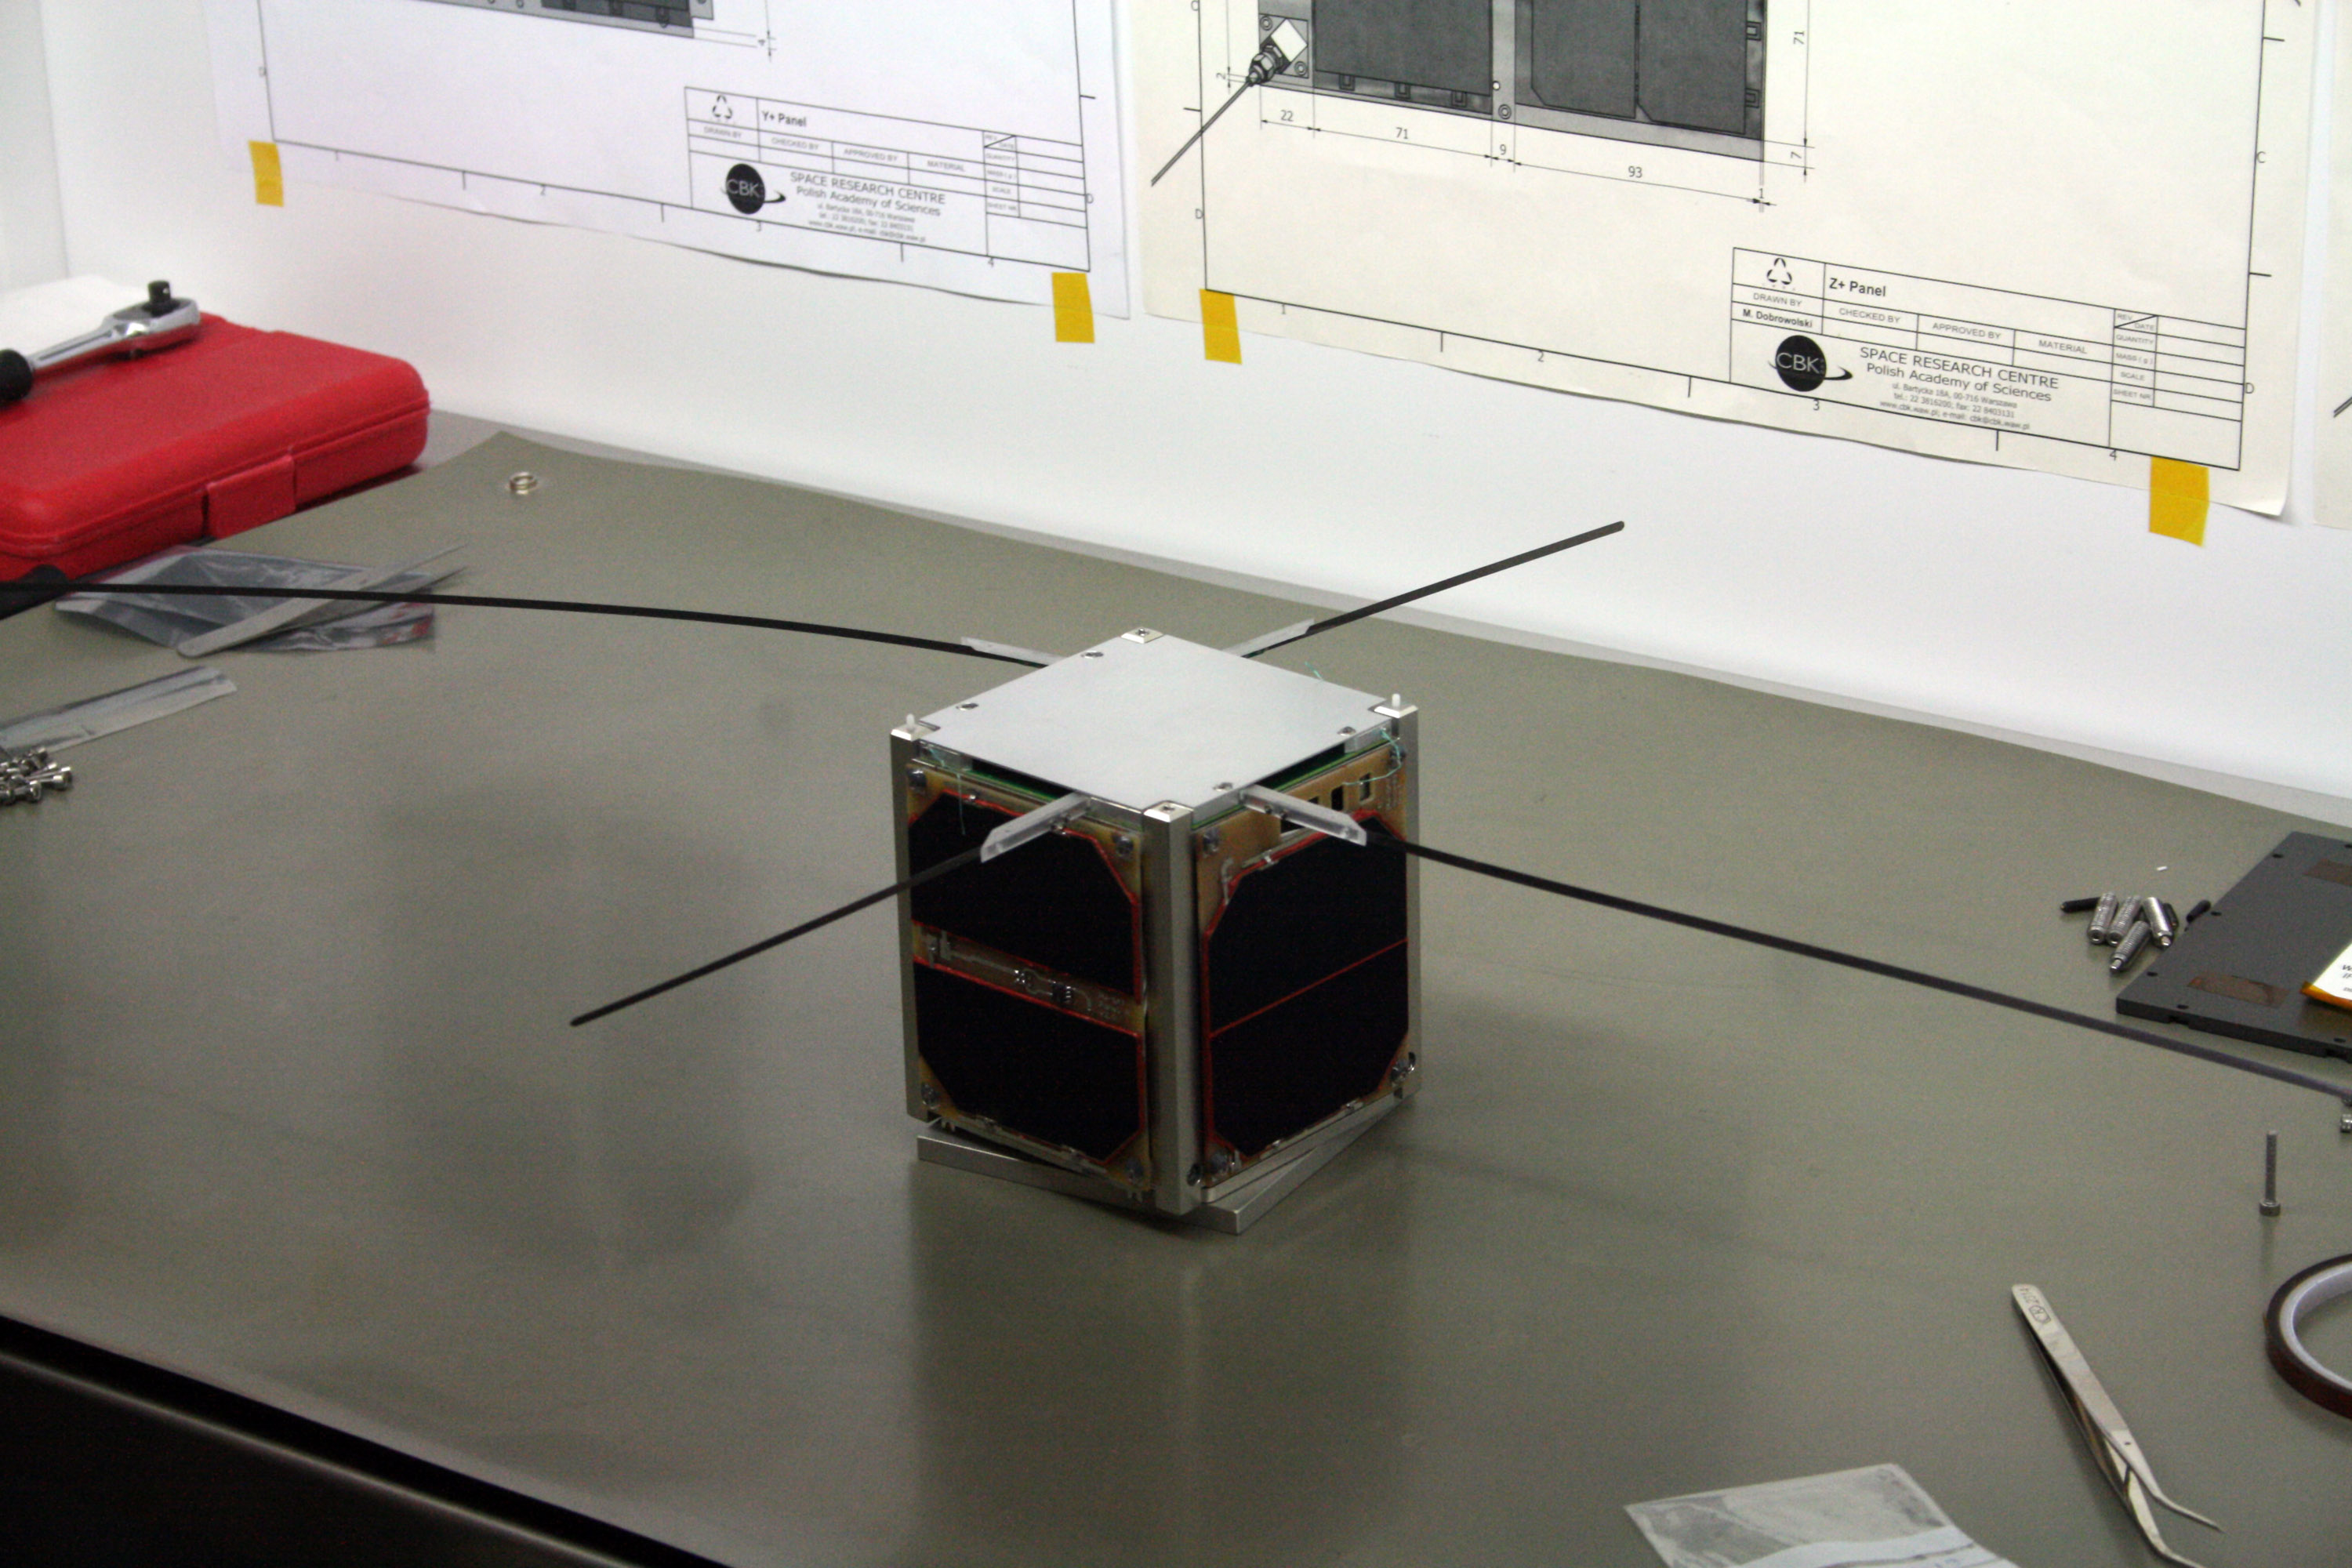
\includegraphics[width=0.32\paperwidth]{img/4/pw-sat1.jpg}
            \caption{PW-Sat1. Source: \cite{pwsat1_website_ska}}
            \label{PW-Sat1_pic}
        \end{figure}
    \end{minipage}
\end{minipage}

\subsection{SwissCube}
SwissCube is the first Swiss satellite, launched in 2009. SwissCube is 1U CubeSat, with two monopole antennas (VHF + UHF) rolled on one panel and deployed on-orbit. Housekeeping data downlink (basic telemetry) use constant \si{10}~WPM Morse code, with \SI{120}{\milli\watt} output power at \SI{437}{\MHz}. Full operational data is sent using \SI{1}{\watt} FSK modulation, \SI{1200}{\bps}. Uplink use FM-modulated AFSK signal on VHF. 

SwissCube use two Ground Stations, one at EPFL, and one at HE-Fribourg. The HE-Fribourg ground station uplink has \SI{11.4}{\dBi} of antenna-gain (one crossed \si{9}-element yagi). The downlink has \SI{14.5}{\dBi} of antenna gain (one crossed \si{17}-element yagi). The second ground station is located at EPFL in Lausanne. The performances of the EPFL ground station are slightly higher than the performances of the Fribourg ground station as there are \si{4} \si{70}-cm yagi antennas in reception (\SI{20.4}{\dBi} gain) and \si{2} \si{2}-m yagi antennas in emission (\SI{13}{\dBi} gain). \cite{swisscube_groundstation}

\begin{minipage}{\linewidth}
    \centering
    \begin{minipage}{0.45\linewidth}
        \begin{figure}[H]
            \centering
            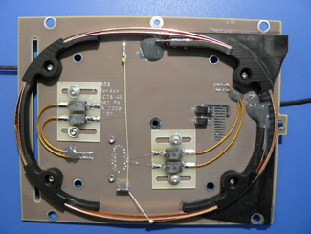
\includegraphics[width=0.32\paperwidth]{img/4/swisscube_stowed.png}
            \caption{SwissCube antennas in the stowed configuration. Source: \cite{swisscube_stowed}}
            \label{swisscube_stowed}
        \end{figure}
    \end{minipage}
    \hspace{0.05\linewidth}
    \begin{minipage}{0.45\linewidth}
        \begin{figure}[H]
            \centering
            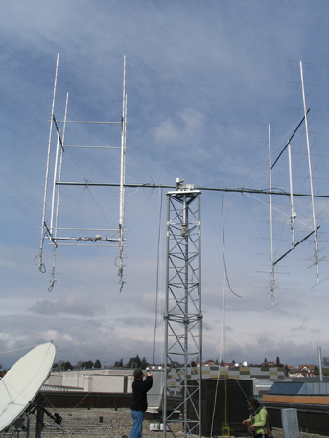
\includegraphics[width=0.32\paperwidth]{img/4/swisscube_groundstation.png}
            \caption{SwissCube EPFL ground station antennas. Source: \cite{swisscube_groundstation}}
            \label{PW-swisscube_groundstation}
        \end{figure}
    \end{minipage}
\end{minipage}
%\chapter{System design}

%In this chapter, design of the radio link and component selection are described. During the design process, multiple iteration of component selection, validation and link budget calculation were made, this chapter describes the final result of the design.

\chapter{System requirements}
\section{Communication sessions}
PW-Sat2 was designed to be deployed on \SI{600}{\kilo\meter}, Sun-synchronous, polar orbit. Due to the Earts rotation, ground station coverage is bounded, and communication with the satellite is limited to communication session during satellite overpass.

Simulations performed using Gpredict software \cite{gpredict_website} shown that communication sessions will happen \si{5}-\si{6} times per day, \si{5}-\SI{10}{\minute} each. This summarizes to the total communication time to average \SI{30}{\minute} per day. Typical radio coverage of the satellite is shown in the figure \ref{gpredict_pass}.

\begin{figure}
    \centering
    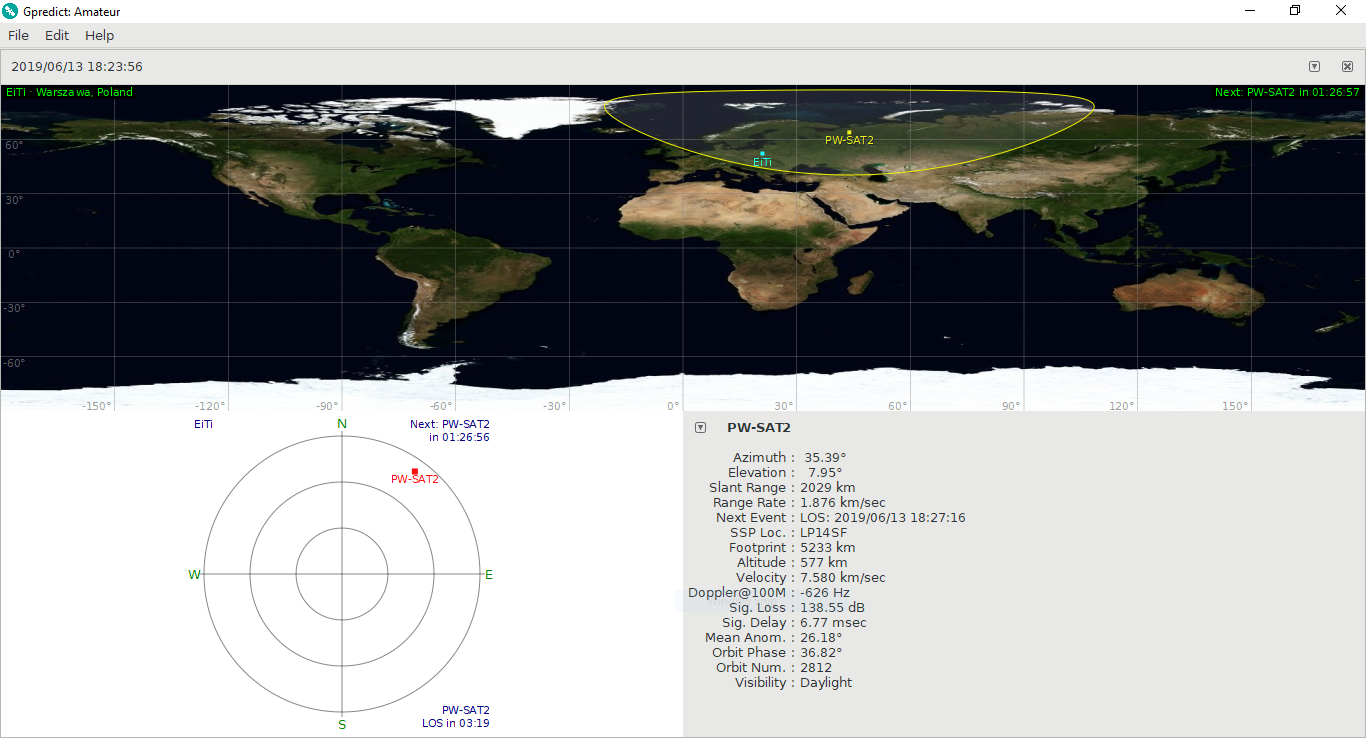
\includegraphics[width=0.8\paperwidth]{img/5/gpredict_pass.png}
    \caption{PW-Sat2 pass in Gpredict software.}
    \label{gpredict_pass}
\end{figure}


\section{Data link budget}
PW-Sat2 have couple of data sources to be sent to the ground, and each of them needs to be taken into account for estimating the required transmission throughput. For each data source the average throughput during ground station coverage is calculated, assuming \SI{30}{\minute} contact per day.
\begin{itemize}
    \item housekeeping telemetry (satellite health information, such as temperatures, bus and solar panel voltages and currents, subsystem status etc. Telemetry is \SI{230}{\byte} frame and should be transmitted every \SI{1}{\minute} (average \SI{30}{\bps}),
    \item archival housekeeping telemetry (gathered during orbit, when no ground station is in range), telemetry should be downloaded in \SI{5}{\minute} step from the whole operational time, which sums up to \SI{64}{\kilo\byte} per day (average \SI{300}{\bps}),
    \item experiment data, which are started by the operator from the ground and each of them is planned to run once a week (Sun Sensor -  \SI{32}{\kilo\byte}, RadFET - \SI{4}{\kilo\byte}, Cameras (10 photos) - \SI{300}{\kilo\byte}) - it sums up to \SI{336}{\kilo\byte} per week, average of \SI{220}{\bps},
    \item Sail deployment procedure, which transmits experiment data on-line (during the experiment). Estimated data to be transmitted (sail deployment indicator, photos and gyroscopes) is about \SI{1}{\kbps}.
\end{itemize}

Data downlink throughput requirement for PW-Sat2 mission sums up to about \SI{1}{\kbps}.
For uplink, the telecommands sent from the ground are relatively short (less than \SI{200}{\byte} each) and the rate of thelecommands is low. Therefore, no specific requirement was created, with minimal usable rate of about \SI{100}{\bps}.

\section{Frequency band selection}



\section{Communication link parameters}
Selected satellite radio module (as described in \autoref{section:comm_design}) imposes the modulation and data packets used in the communication. This section briefly describes used modulations, frame formats and implications to the ground segment of the system.

\subsection{Downlink modulation}
Downlink signal is modulated using Binary Phase Shift Keying (BPSK). The data rate can be changed dynamically by the spacecraft On-Board Computer, in range \si{1.2} - \SI{9.6}{\kbps}, allowing to improve the link quality when necessary. Baseband signal is also filtered using Raised Root Cosine filter, to reduce side lobes power. Signal bandwidth varies between \SI{2.4}{\kHz} (for \SI{1.2}{\kbps}) and \SI{19.2}{\kHz} (for \SI{9.6}{\kbps}).

% TODO: rysunek BPSK

\subsection{Uplink}
Uplink modulation is two-staged: first, data is modulated using Frequency Shift Keying with Bell 202 modem tones (0s and 1s translated to tones \SI{1200}{\hertz} and \SI{2200}{\hertz}), later to be Frequency Modulated on the RF carrier (with frequency deviation of $\pm\SI{5}{\kilo\hertz}$).

% TODO: schemat modulatora

\subsection{Frame format}
Physical layer data format is reduced-functionality AX.25 packet \cite{AX25_standard}. Only connectionless transmission mode and UI frames are supported. Packet framing is the same as in SwissCube CubeSat \cite{SwissCube_AX25}.

Basic frame format is shown in the table \ref{AX25_frame}. All the fields except flags are bit-stuffed to ensure that the \textit{Flag} field does not appear in the data: if there are six '1' bits to be send, transmitter inserts '0' bit before the last one. Adressing in this system in inherent, but unused - this is point-to-point connection, therefore adresses are fixed. Frame-Check Sequence is a CRC (CITT standard) of the whole frame (without \textit{Flags}). \textit{Information Field} is variable-length, between \si{4} and \SI{256}{\byte} length is the place for the actual data transmitted by the On-Board Computer.

\begin{table}
\small
\centering
\caption{AX.25 frame format}
\label{AX25_frame}
\arrayrulecolor{black}
\begin{tabular}{l|c|c|c|c|c|c|c|c|} 
\hhline{~|-|----|-|-|-|}
\multirow{2}{*}{}                                                              & \multirow{2}{*}{Flag } & \multicolumn{4}{c|}{AX.25 Transfer Frame Header (128 bits)}                                                                                                                                                                                   & {\cellcolor[rgb]{0.753,0.753,0.753}}                                                                                                                  & \multirow{2}{*}{\begin{tabular}[c]{@{}c@{}}Frame-\\Check\\Sequence\end{tabular}} & \multirow{2}{*}{Flag}  \\ 
\hhline{~|~|-|-|-|-|>{\arrayrulecolor[rgb]{0.753,0.753,0.753}}->{\arrayrulecolor{black}}|~|~|}
                                                                               &                        & \begin{tabular}[c]{@{}c@{}}Destination\\Address\end{tabular} & \begin{tabular}[c]{@{}c@{}}Source\\Address\end{tabular} & \begin{tabular}[c]{@{}c@{}}Control\\Bits\end{tabular} & \begin{tabular}[c]{@{}c@{}}Protocol\\Identifier\end{tabular} & \multirow{-2}{*}{{\cellcolor[rgb]{0.753,0.753,0.753}}\begin{tabular}[c]{@{}>{\cellcolor[rgb]{0.753,0.753,0.753}}c@{}}Information\\Field\end{tabular}} &                                                                                  &                        \\ 
\hline
\multicolumn{1}{|c|}{\begin{tabular}[c]{@{}c@{}}Length\\{[}bits]\end{tabular}} & 8                      & 56                                                           & 56                                                      & 8                                                     & 8                                                            & {\cellcolor[rgb]{0.753,0.753,0.753}}32-2048                                                                                                           & 16                                                                               & 8                      \\ 
\hline
\multicolumn{1}{|c|}{Value}                                                    & 01111110               & PWSAT2-0                                                     & PWSAT2-0                                                & 00000011                                              & 11110000                                                     & {\cellcolor[rgb]{0.753,0.753,0.753}}                                                                                                                  & CRC-CITT                                                                         & 01111110               \\
\hline
\end{tabular}
\end{table}


Additionally, downlink data is scrambled using G3RUH scrambling polynomial to maximize randomness and ensure proper bit synchronization.

% \subsection{Flatsat}

% Most of the tests were performed on Flatsat (an abbreviation from Flat Satellite), an electronic test bench, which consist of mix of flight models, engineering models of the instruments and Electrical Ground Support Equipment (EGSE). EGSE are the test instruments and/or mocks (fake) instruments, which allow testing without the need for actual hardware.

% PW-Sat2 Flatsat was integrated in Space Research Centre in Warsaw. Flatsat is shown in the figure \ref{TODO}.

% \subsubsection{Flatsat Ground Station mock}
% To perform the communication tests a Ground Station mock was created of flatsat. It was built using to Software-Defined Radios: one, as downlink receiver, same as to be installed in the Ground Station (Funcube Pro+), and the second (PlutoSDR) to generate uplink signals. Use of SDR instead of analogue radio transceiver greatly simplified the tests performed. Ground station mock is shown in the figure \ref{TODO}. 




\chapter{Space segment}
Space segment is a part of the satellite communication system that resides on the satellite itself. It is divided into two main parts: communication subsystem (COMM) and antennas (ANTs) connected with two coaxial cables.

Space segment is critical in system operation and reliability - there is no possibility to carry out any repairs, perform maintenance or adjustment once on orbit. It is exposed to the space environment - wide temperature range, thermal cycling, cosmic radiation and vacuum.

Because of the mentioned requirements it was decided to choose commercially available and flight-proven CubeSat components to increase the overall reliability of the system.

% -----------------------------------------------------------------------------------------------------------
% -----------------------------------------------------------------------------------------------------------
% -----------------------------------------------------------------------------------------------------------

\section{Spacecraft communication transceiver}
\label{section:comm_design}
CubeSat design specification \cite{cubesat_spec}, with which PW-Sat2 is compliant, defines common PC/104 connector, which is the main data bus for all satellite subsystems. On the connector, two \iic and two CAN buses are defined and most of the components are compatible to each other. However, due to the lack of CAN interface on On-Board Computer (CubeComputer from CubeSpace \cite{cubespace_website}) radio should use \iic communication bus.

When the subsystem was ordered (in year \si{2014}), the choice of available products was very limited, and the only radio which was compliant with above mentioned requirements was ISIS VHF uplink/UHF downlink Full Duplex Transceiver. Its view and block diagram is shown in the figures \ref{ISIS_TRXvU_photo} and \ref{ISIS_TRXvU_block_diagram}.

\begin{figure}
    \centering
    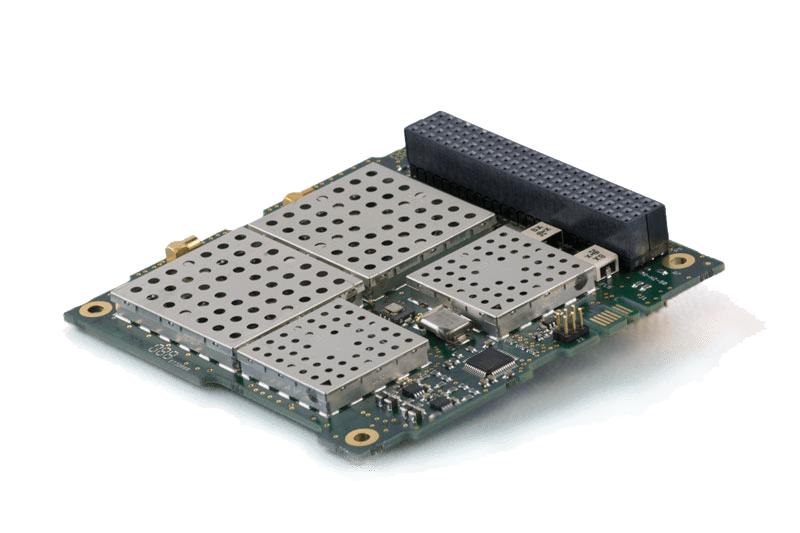
\includegraphics[width=0.5\paperwidth]{img/6/ISIS-radio-UHF-VHF-min.png}
    \caption{ISIS VHF uplink/UHF downlink Full Duplex Transceiver photo. Source: \cite{isis_trxvu}}
    \label{ISIS_TRXvU_photo}
\end{figure}

\begin{figure}
    \centering
    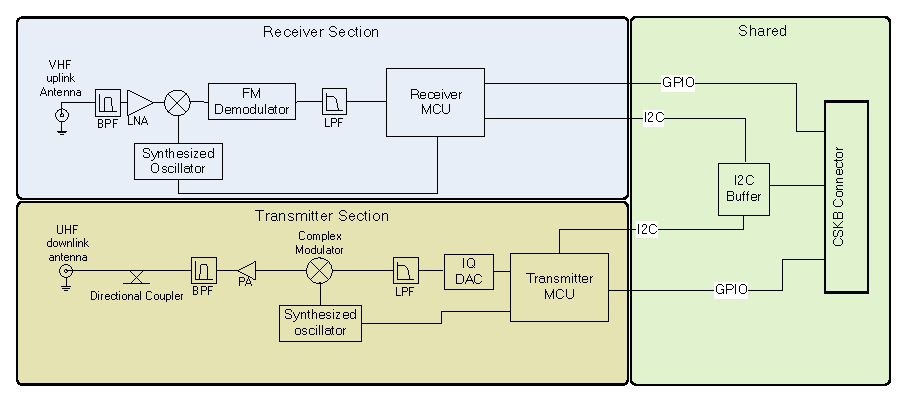
\includegraphics[width=0.8\paperwidth]{img/6/ISIS_TRXvU_block_diagram.eps}
    \caption{ISIS VHF uplink/UHF downlink Full Duplex Transceiver block diagram. Source: \cite{isis_trxvu}}
    \label{ISIS_TRXvU_block_diagram}
\end{figure}

Basic characteristics: \\
\begin{tabular}{c|c}
     \textbf{downlink} & \textbf{uplink} \\ \hline
     \multicolumn{2}{c}{dual-\iic ~communication standard} \\
     \multicolumn{2}{c}{AX.25 frame format} \\
     \si{430}-\SI{450}{\MHz} frequency range & \si{140}-\SI{150}{\MHz} frequency range \\
     \SI{0.5}{\watt} downlink power & \SI{-98}{\dBm} sensitivity for \si{10^-5}~BER \\
     \si{1.2} - \SI{9.6}{\kilo\bit / \second} bitrate & \SI{1.2}{\kilo\bit / \second} bitrate \\ 
     BPSK modulation with G3RUH scrambling & FM-modulated AFSK \\ 
\end{tabular}

Transceiver was tested separately for its uplink and downlink capabilities. Tests are critical to make sure that radio parameters are maintained in the system, and to verify manufacturers' data.

\subsection{Sensitivity measurement}
Sensitivity was measured by the setup shown in the figure \ref{4_uplink_sensitivity}. Test procedure:

\begin{itemize}
    \item measuring output power of PlutoSDR using spectrum analyzer with wide RBW filter (\SI{1}{\MHz}),
    \item calculating input power to the Communications module,
    \item PER is calculated by transmitting data frames using PlutoSDR (with GNUradio) and receing them by On-Board Computer connected to the PC,
    \item decreasing output power of PlutoSDR and measuring PER for each point (\si{1000}~frames).
\end{itemize}

\begin{figure}
    \centering
    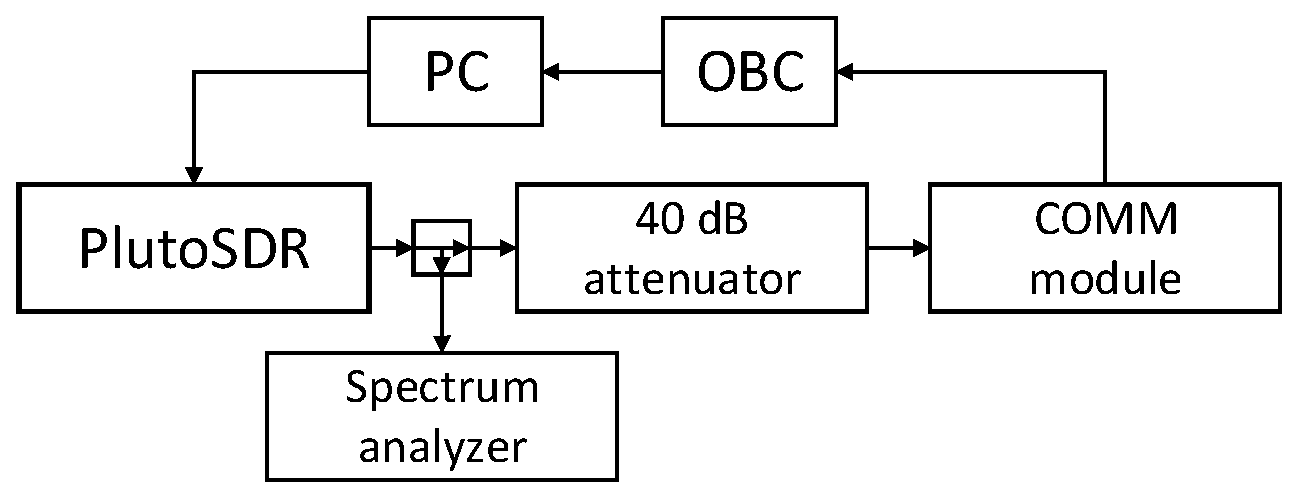
\includegraphics[width=0.6\paperwidth]{img/6/uplink_sensitivity.eps}
    \caption{Uplink sensitivity measurement block diagram.}
    \label{4_uplink_sensitivity}
\end{figure}

Measured PER chart is shown in the figure \ref{4_uplink_sensitivity_graph}. It is compared to the ideal BFSK curve. For usable PER of about \SI{1}{\percent} the sensitivity of the communication module is \SI{-95}{\dBm}.

\begin{figure}
    \centering
    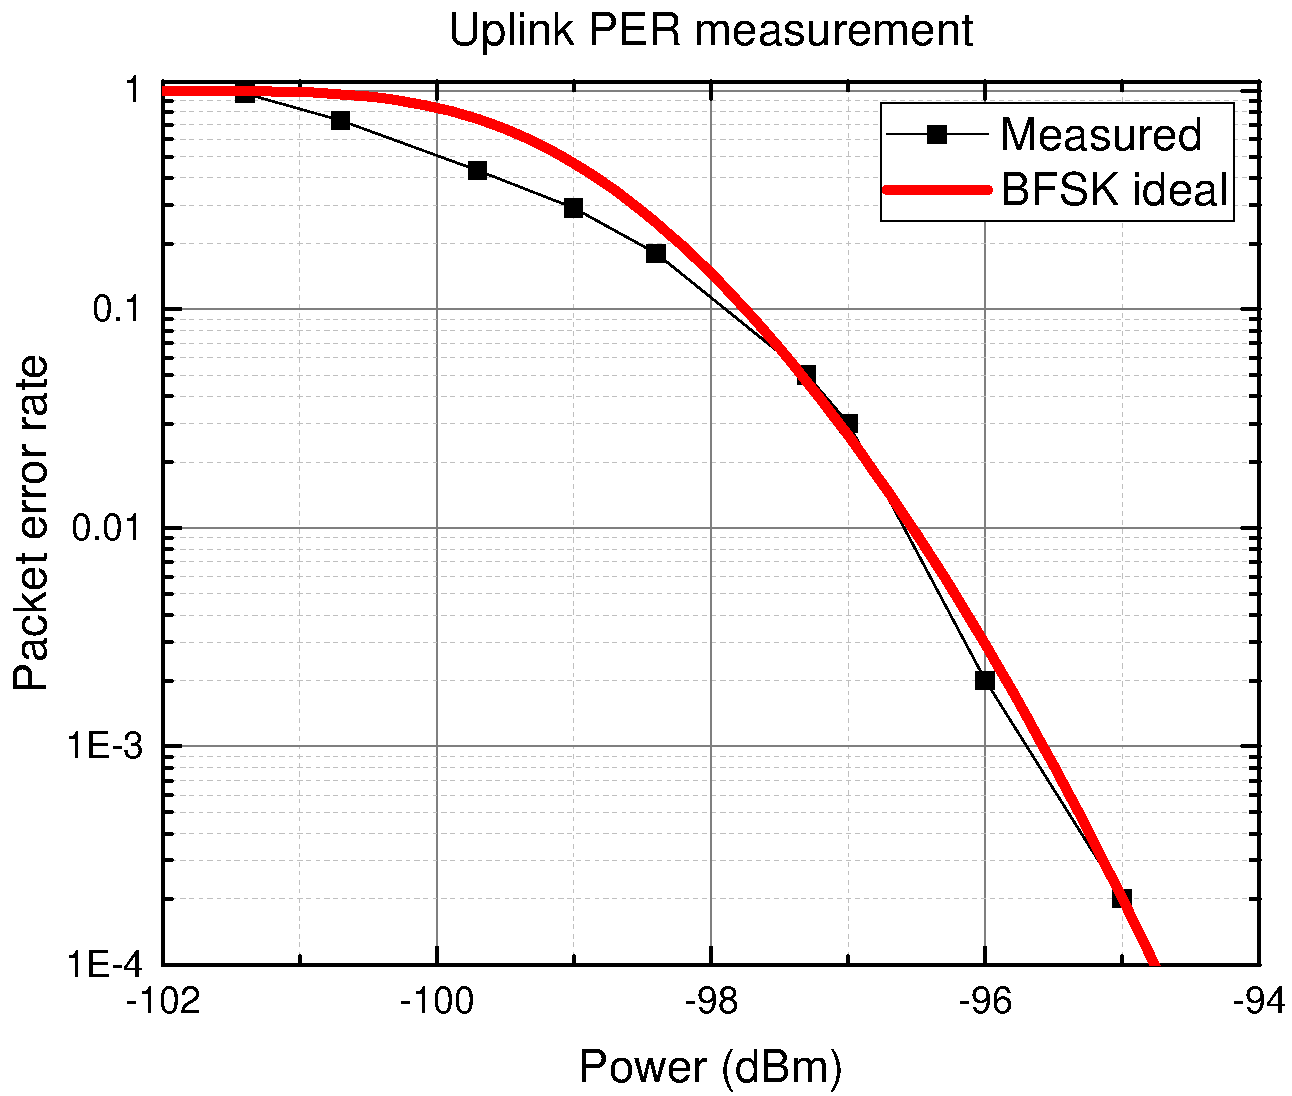
\includegraphics[width=0.8\paperwidth]{img/6/uplink_per.pdf}
    \caption{Uplink sensitivity measurement.}
    \label{4_uplink_sensitivity_graph}
\end{figure}


\subsection{Doppler effect influence on uplink}
Doppler effect is caused when fast-moving object is emitting/receiving radio waves. For uplink frequency (VHF band) Doppler effect influence can shift frequency up to about \SI{5}{\kHz}. The receiver bandwidth should be measured to estimate allowable frequency inaccuracies.

Test setup is the same as in previous setup, shown in the figure \ref{4_uplink_sensitivity}. During the test the PER was measured for a range of frequency offsets from the center frequency of the module. The input power to the module was set to \SI{3}{\dB} above sensitivity level (\SI{-92}{\dBm}) and for each point the number of packets sent was \si{500}.  The result is shown in the chart \ref{4_uplink_doppler_measurement}.

\begin{figure}
    \centering
    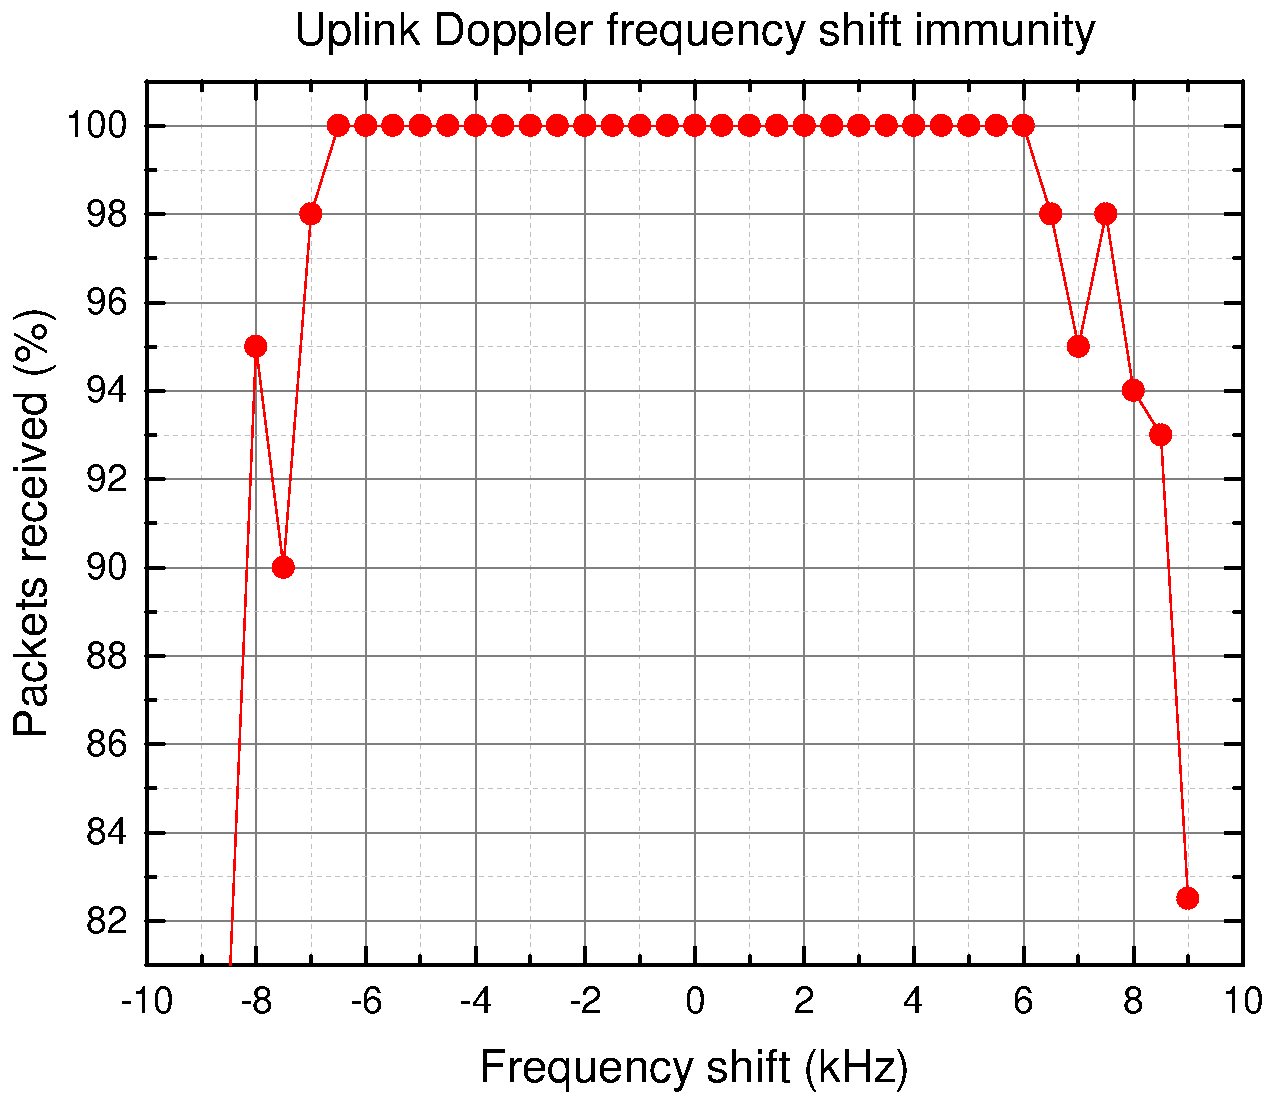
\includegraphics[width=0.6\paperwidth]{img/6/uplink_doppler.pdf}
    \caption{Uplink Doppler effect influence measurement.}
    \label{4_uplink_doppler_measurement}
\end{figure}


\subsection{Transmitter spectrum and output power}
Output power was measured using spectrum analyzer with wide resolution bandwidth. Output power was measured to be \SI{28}{\dBm}, which is in the manufacturers specification.
The spectrum of the signal was recorded, showing significant side lobes (first lobe TODO\SI{10}{\dB} lower than main carrier).
TODO





% -----------------------------------------------------------------------------------------------------------
% -----------------------------------------------------------------------------------------------------------
% -----------------------------------------------------------------------------------------------------------



\section{Spacecraft Antennas}
Because of the selected radio system, two antennas has to be installed - one for uplink (VHF) and one for downlink (UHF). Antennas should be omnidirectional, as PW-Sat2 does not have an nadir-pointing capability and random tumbling during operation is assumed.

Self-made dipole antenna was considered at the design stage, but due to mechanical and time constraints, satellite antenna was decided to be bought as well. Innovative Solutions In Space company sells antenna with with the transceiver as CubeSat communication Kit \texttt{CubeSat dipole antenna system}. Both elements are compatibile and the whole system (transceiver + antenna) is tuned for specific communication frequency and mounting option.

This system is deployable by the command from the on-board computer. Thermal knife (resistor) is heated up and thermal link is burnt, resulting is antenna deploy by the spring action. Antenna is shown in the figure \ref{ISIS_antenna}.

\begin{figure*}
   \centering
\begin{tabular}{cc}
        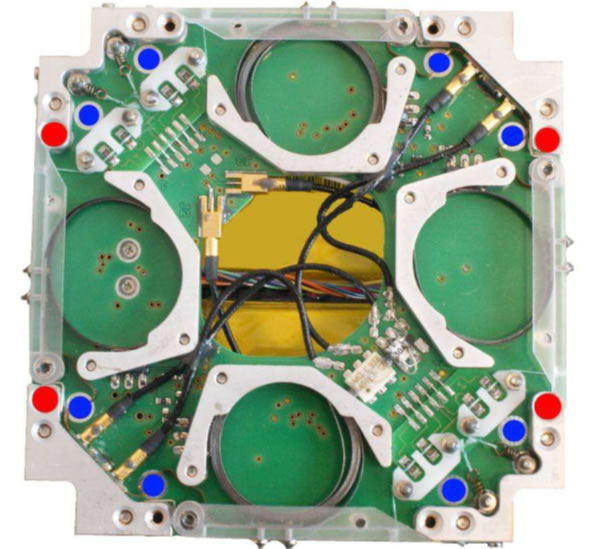
\includegraphics[width=0.3\paperwidth]{img/6/isis_antenna_stowed.jpg}
    & 
        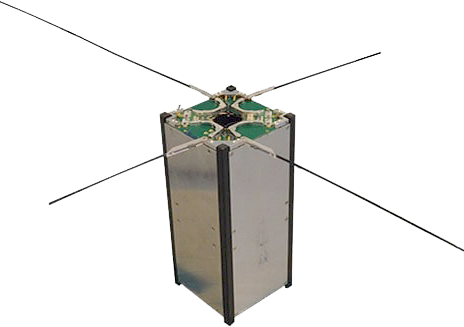
\includegraphics[width=0.45\paperwidth]{img/6/CubeSat-antenna-dipole-configuration.png}    
\end{tabular}
\label{ISIS_antenna}
\caption{ISIS CubeSat dipole antenna system in stowed and deployed position. Source: \cite{isis_dipole_antenna}}
\end{figure*}


\subsection{Measurements}
First automatic task of the satellite it to deploy the antennas. During the test campaign antenna deployment procedure was executed four times, due to the issues with Antenna opening. Satellite during antenna deployment is shown in the figure \ref{pwsat_with_deployed_antennas}.

\begin{figure}
    \centering
    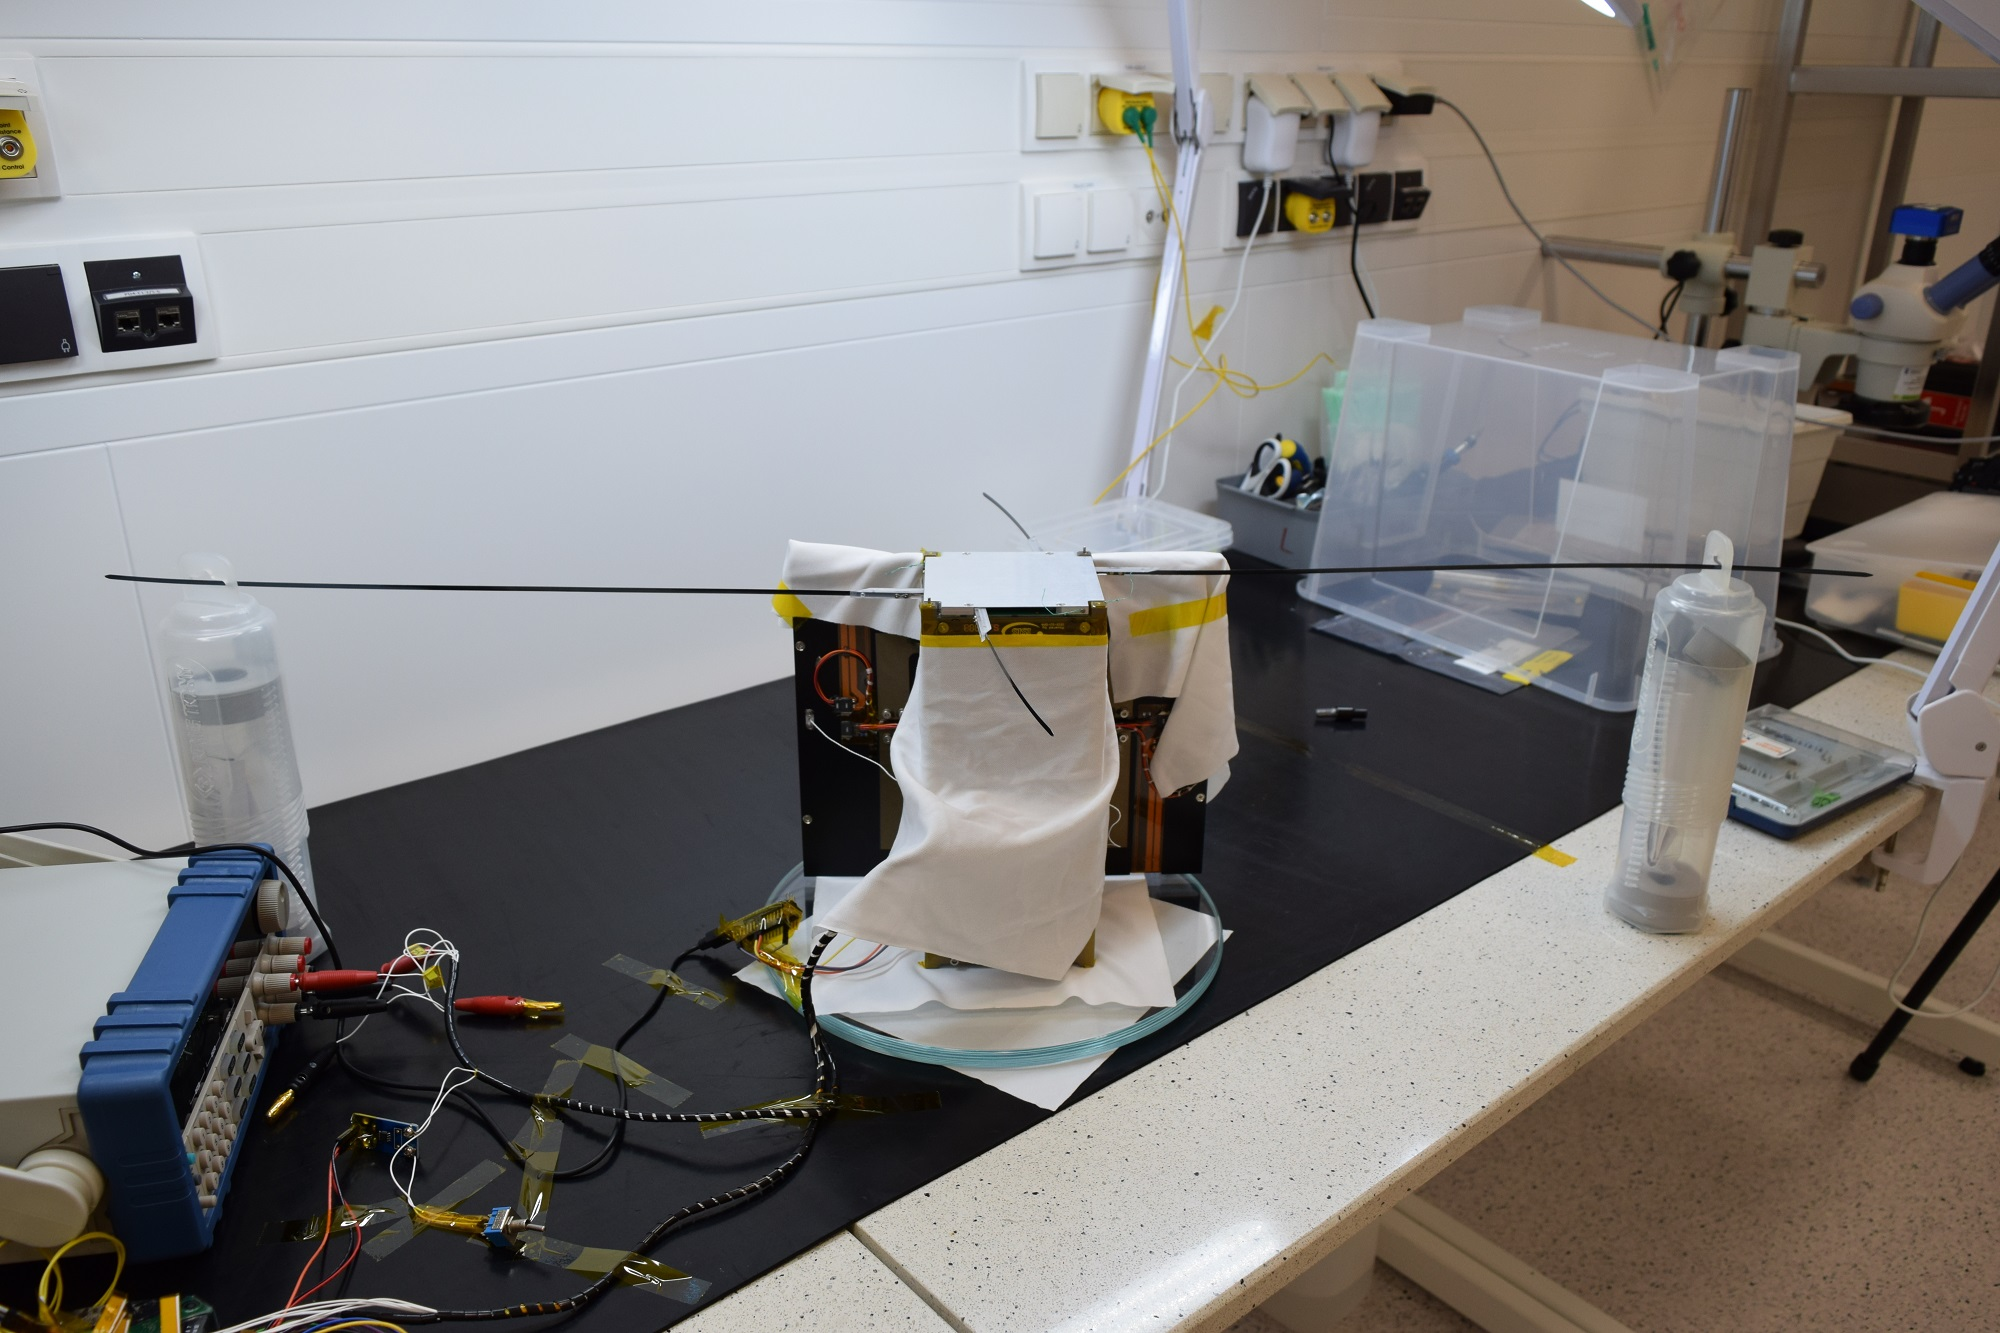
\includegraphics[width=0.6\paperwidth]{img/6/pwsat_with_deployed_antennas.JPG}
    \caption{PW-Sat2 with deployed solar panels during antenna verification.}
    \label{pwsat_with_deployed_antennas}
\end{figure}

Manufacturer of the antennas provide a test report with the measured antennas matchins ($s_{11}$ parameter), for VHF and UHF frequencies they are shown in the figures \ref{isis_s11_vhf} and  \ref{isis_s11_uhf}, respectively.

\begin{figure}
    \centering
    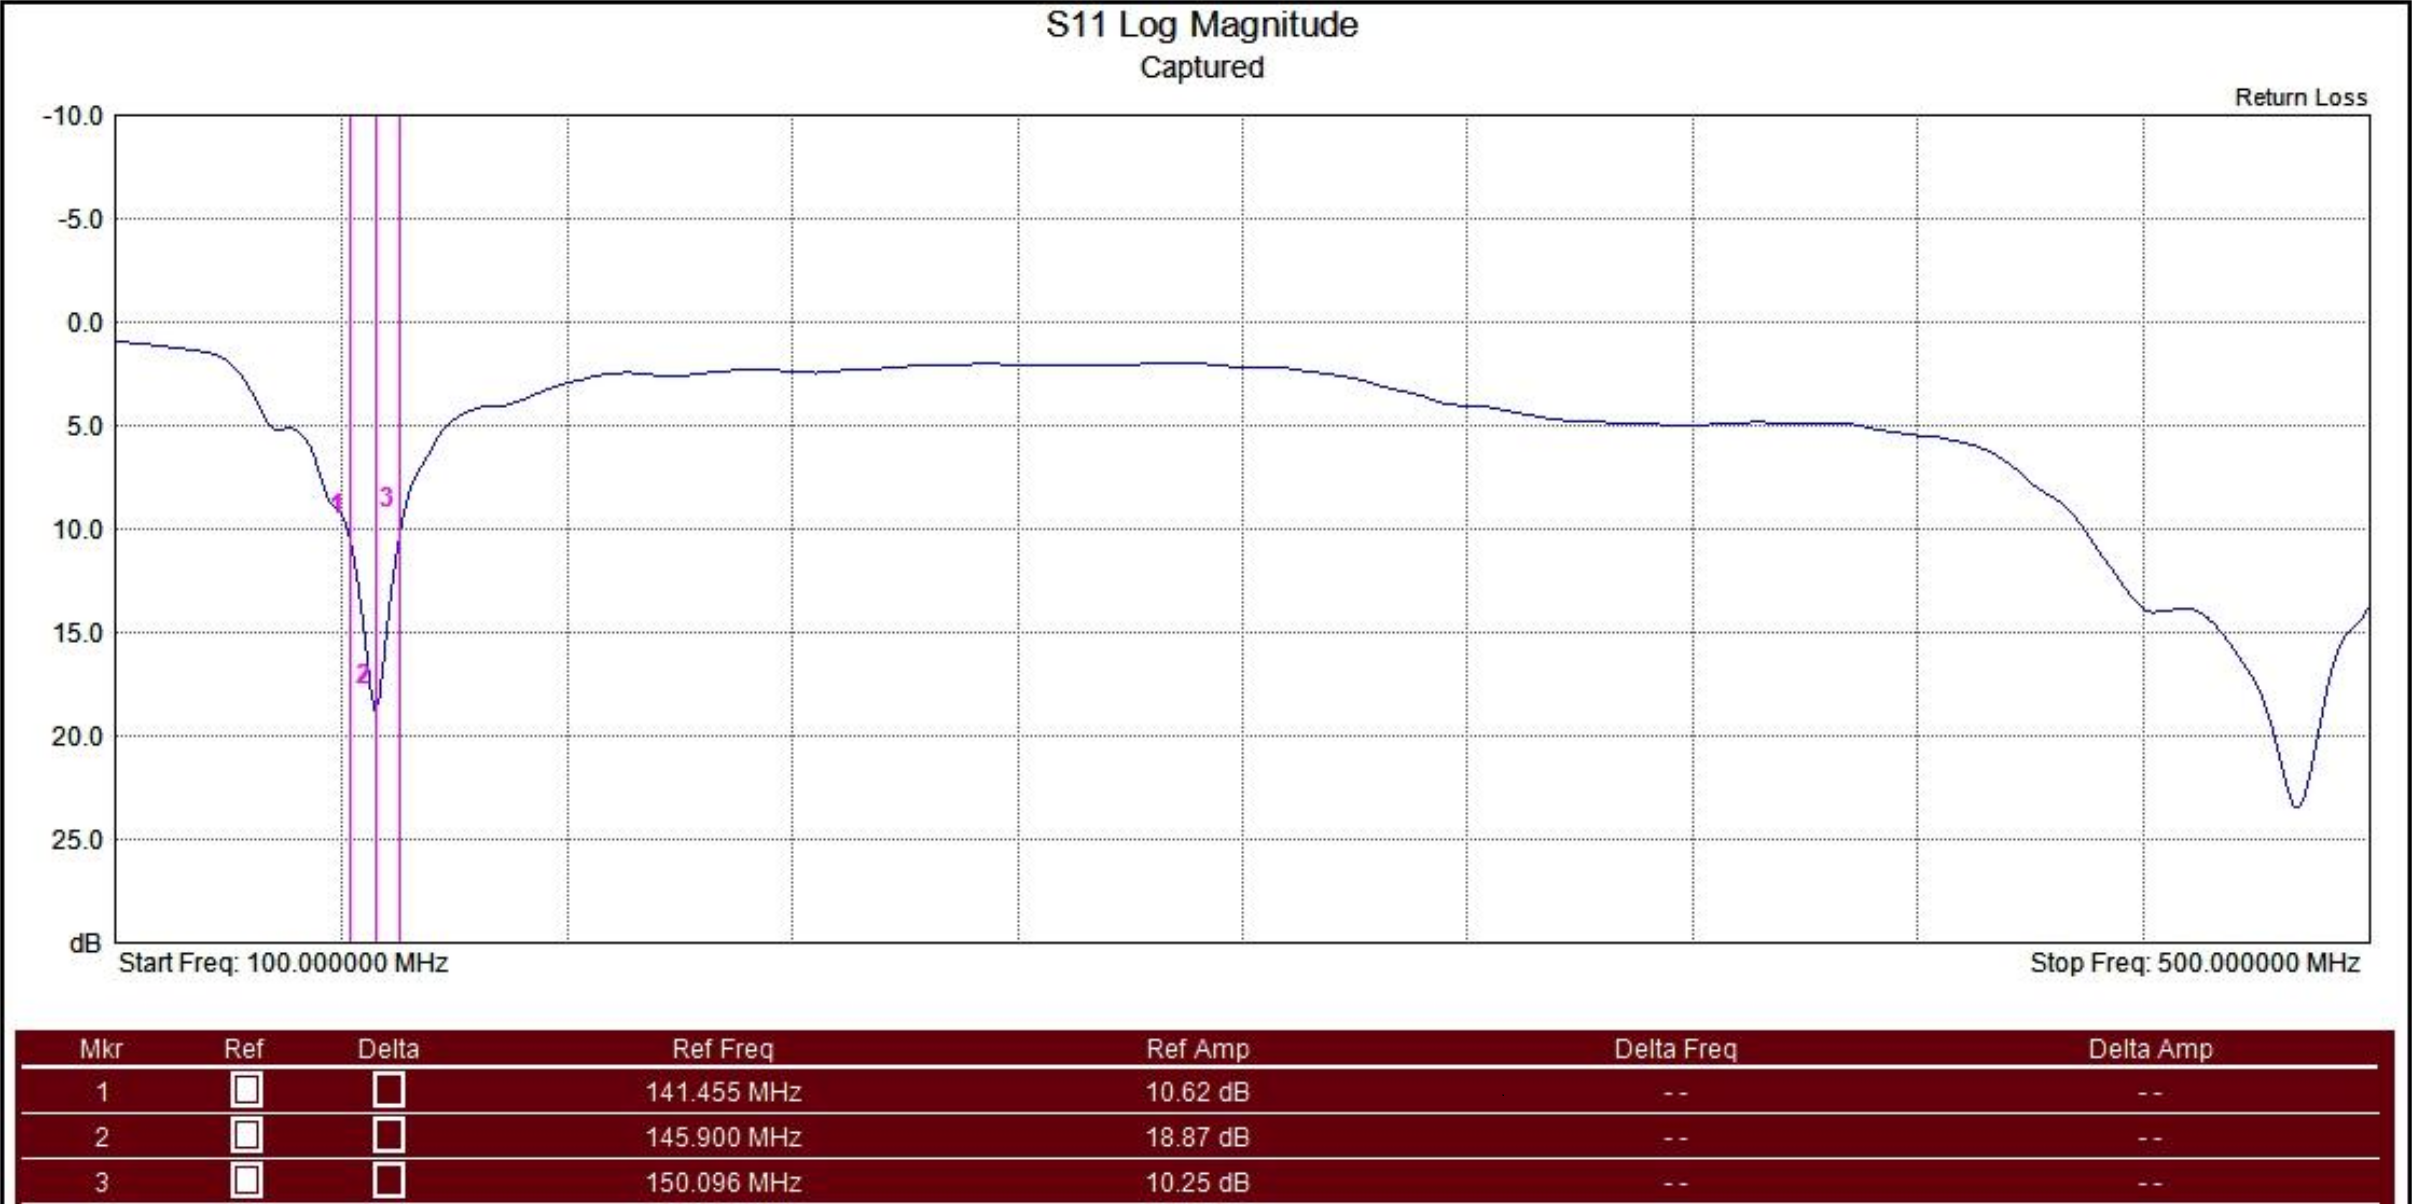
\includegraphics[width=0.8\paperwidth]{img/6/isis_s11_vhf.png}
    \caption{VHF antenna matching. Source: \cite{isis_ant_test_report}}
    \label{isis_s11_vhf}
\end{figure}

\begin{figure}
    \centering
    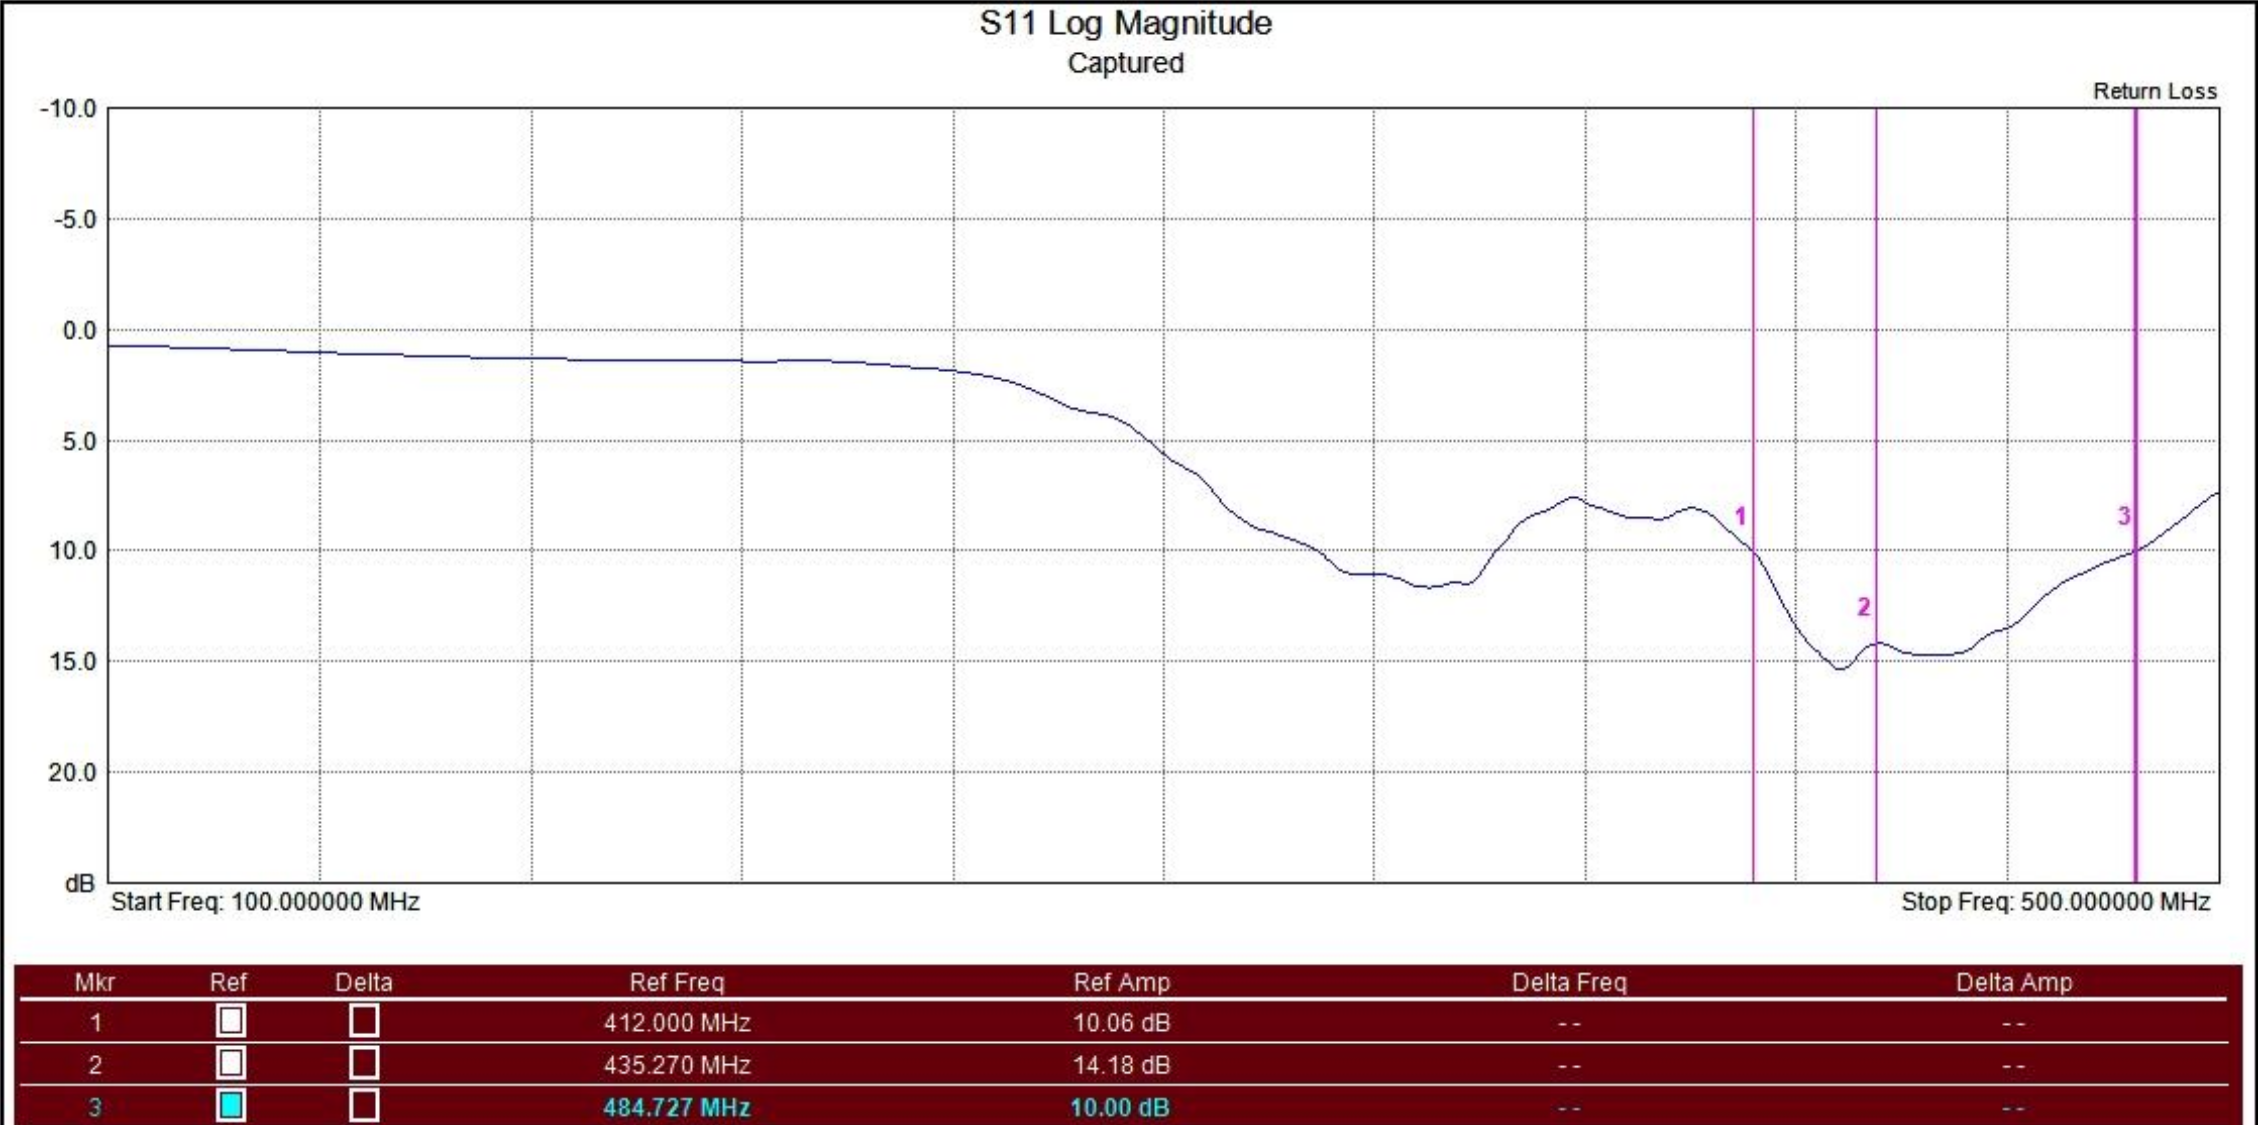
\includegraphics[width=0.8\paperwidth]{img/6/isis_s11_uhf.png}
    \caption{UHF antenna matching. Source: \cite{isis_ant_test_report}}
    \label{isis_s11_uhf}
\end{figure}


Both forward and reflected power from the antenna are measured by the radio module during radio frame transmission. Correct antenna deployment can be verified also by using the telemetry. During the test antenna deployment both forward and reflected power were captured. Average measured value of the forward power: \textbf{\SI{28.8}{\dBm} $\pm$ \SI{0.43}{\dBm}} and reflected power: \textbf{\SI{19.6}{\dBm} $\pm$ \SI{0.54}{\dBm}}. This means that the antenna matching for UHF frequencies is: SWR~$= 2.1$, $s_{11} = -9.2~dB$. This means that the power lost in the mismatch is \SI{0.5}{\dB}. Measured value is similar to measured by the manufacturer ($s_{11} = \SI{-14}{\dB}$).

\subsection{Antennas on orbit}
Reflected and forward power are being captured during the mission, the chart of the reflected and forward power, from the ground testing up to mission completion is shown in the figure \ref{4_rf_power_comm}. This shows that VSWR of the antenna didn't change much during the mission, however Sail and Solar Arrays deploments are clearly seen on the measurements. Picture of the shadow of the satellite on the Sail, showing opened antennas is shown in the figure \ref{antennas_deployed_orbit}.

\begin{figure}
    \centering
    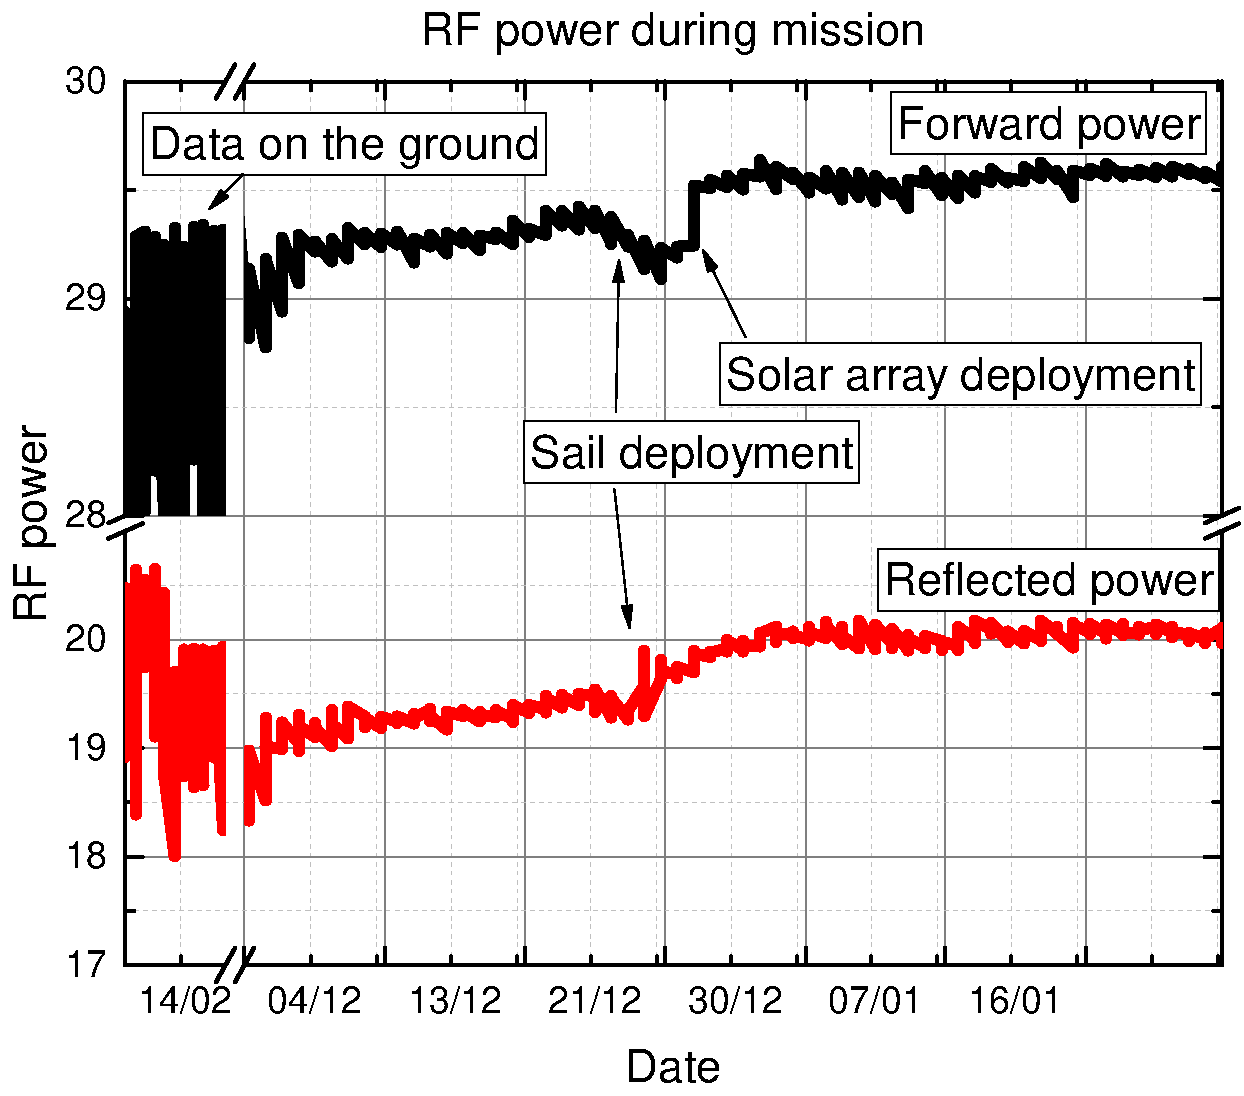
\includegraphics[width=0.6\paperwidth]{img/6/rf_power_comm.pdf}
    \caption{RF power during mission.}
    \label{4_rf_power_comm}
\end{figure}

\begin{figure}
    \centering
    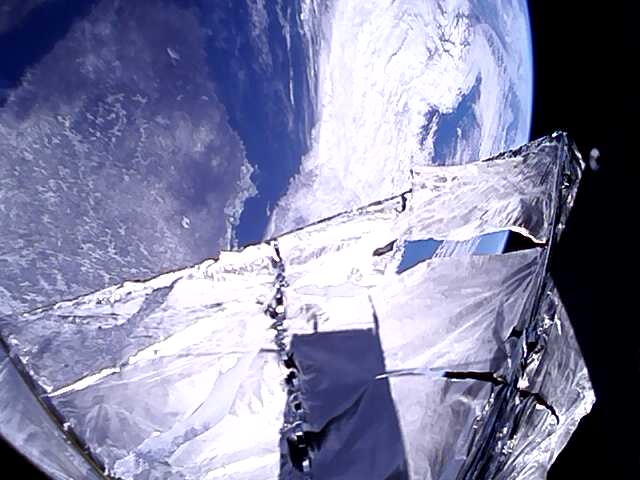
\includegraphics[width=0.7\paperwidth]{img/6/antennas_deployed_orbit.jpg}
    \caption{On-Board photo from PW-Sat2 showing opened antennas.}
    \label{antennas_deployed_orbit}
\end{figure}


% -----------------------------------------------------------------------------------------------------------
% -----------------------------------------------------------------------------------------------------------
% -----------------------------------------------------------------------------------------------------------

% \subsubsection{Deployable elements influence on the antenna pattern}
% TODO

% On-board PW-Sat2 are two main deployables: solar panels and deorbitation sail.

% During design stage, influence of the solar panels was discussed with antenna manufacturer - the outcome was to place longed dipoles (VHF) along the solar panels, and shorter ones orthogonally to it, as shown in the figure \ref{???}

% % TODO: zdjęcie z otwartymi panelami i antenami

% The influence of the deorbit sail was also simulated during Critical Design stage.

% Deorbitation sail is made by very thin (\SI{5}{\micro\meter}) mylar foil with aluminium coating. Using % TODO
% simulation tool, it was shown that the sail will increase directivity of the cubesat antennas, acting as a reflector.
% % TODO: jakieś zdjęcie z symulacji, wynik o ile dB się pogorszyło



\chapter{Ground segment}
Ground station design should complement the space segment, with large antenna gains and output power to allow the budget link to close. As the system is full-duplex, both uplink and downlink channels are separate and the design should allow to simultaneously operate transmit and receive. Block diagram of the designed ground station is shown in the figure \ref{gs_block_diagram}.
Due to the low sensitivity of the satellite receiver (\SI{-97}{\dBm}) uplink EIRP has to be very large. This is achieved by using high-power amplifier and antennas with high directional gain. For downlink, ground station has to compensate low transmit power of the satellite, by using high gain antennas and very sensitive receiver.

Ground station consists of not only the hardware but also software. Many parts of the system use Digital Signal Processing and Software-Defined Radio for data modulation/de-modulation, packet transmission etc. For the DSP tasks, GNUradio \cite{gnuradio} was selected and the tool for sampling-based signal processing.

Ground station is located on the building of Faculty of Electronics and Information Technology, Warsaw University of Technology.

\begin{figure}[H]
    \centering
    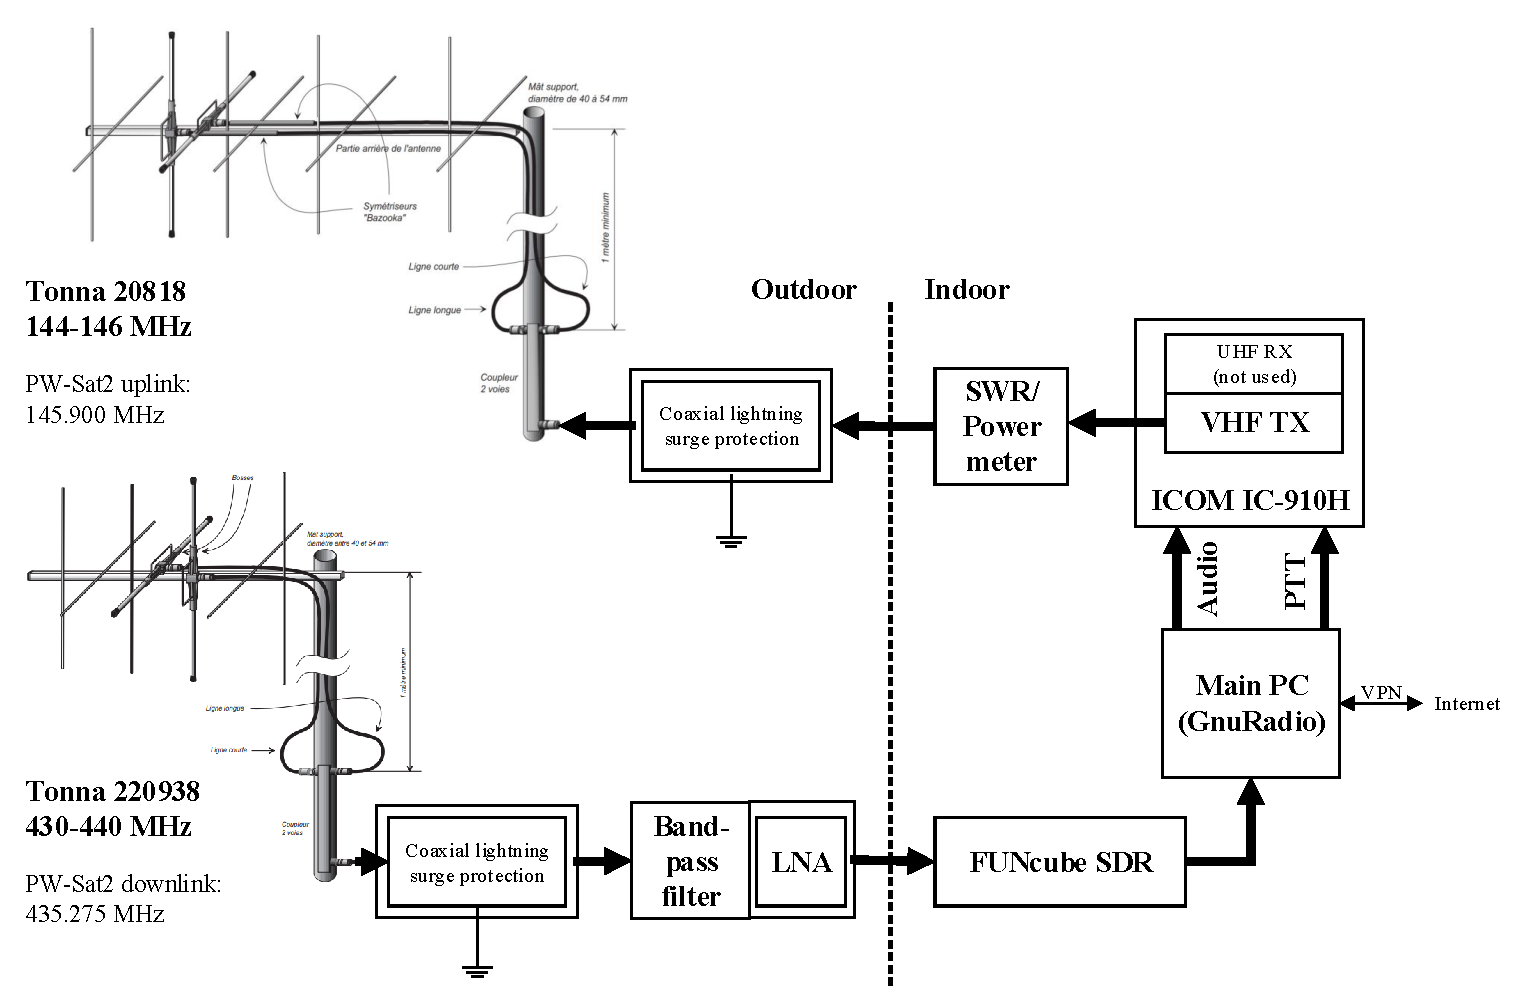
\includegraphics[width=0.7\paperwidth]{img/7/gs_block_diagram.eps}
    \caption{Ground station block diagram}
    \label{gs_block_diagram}
\end{figure}

\section{Antenna mast \& equipment}
Antenna mast \& rotator were already installed from previous experiments with satellite transmission. Main parameters: \SI{3}{\meter} height, SPID rotator with azimuth-elevator control and PC interface. Mast with installed antennas is shown in the figure \ref{elka_antena_mast} and the antenna rotator with nearby elements is shown in the figure \ref{elka_antenna_rotator}. Coaxial lightning surge protector SP3000W installed on the mast is shown in the figure \ref{coax_surge_protection}. This elemnent discharges any high voltage pulses which can happen suring the lightning by the cost of insertion loss (declared \SI{0.2}{\dB}).

\begin{figure}[H]
    \centering
    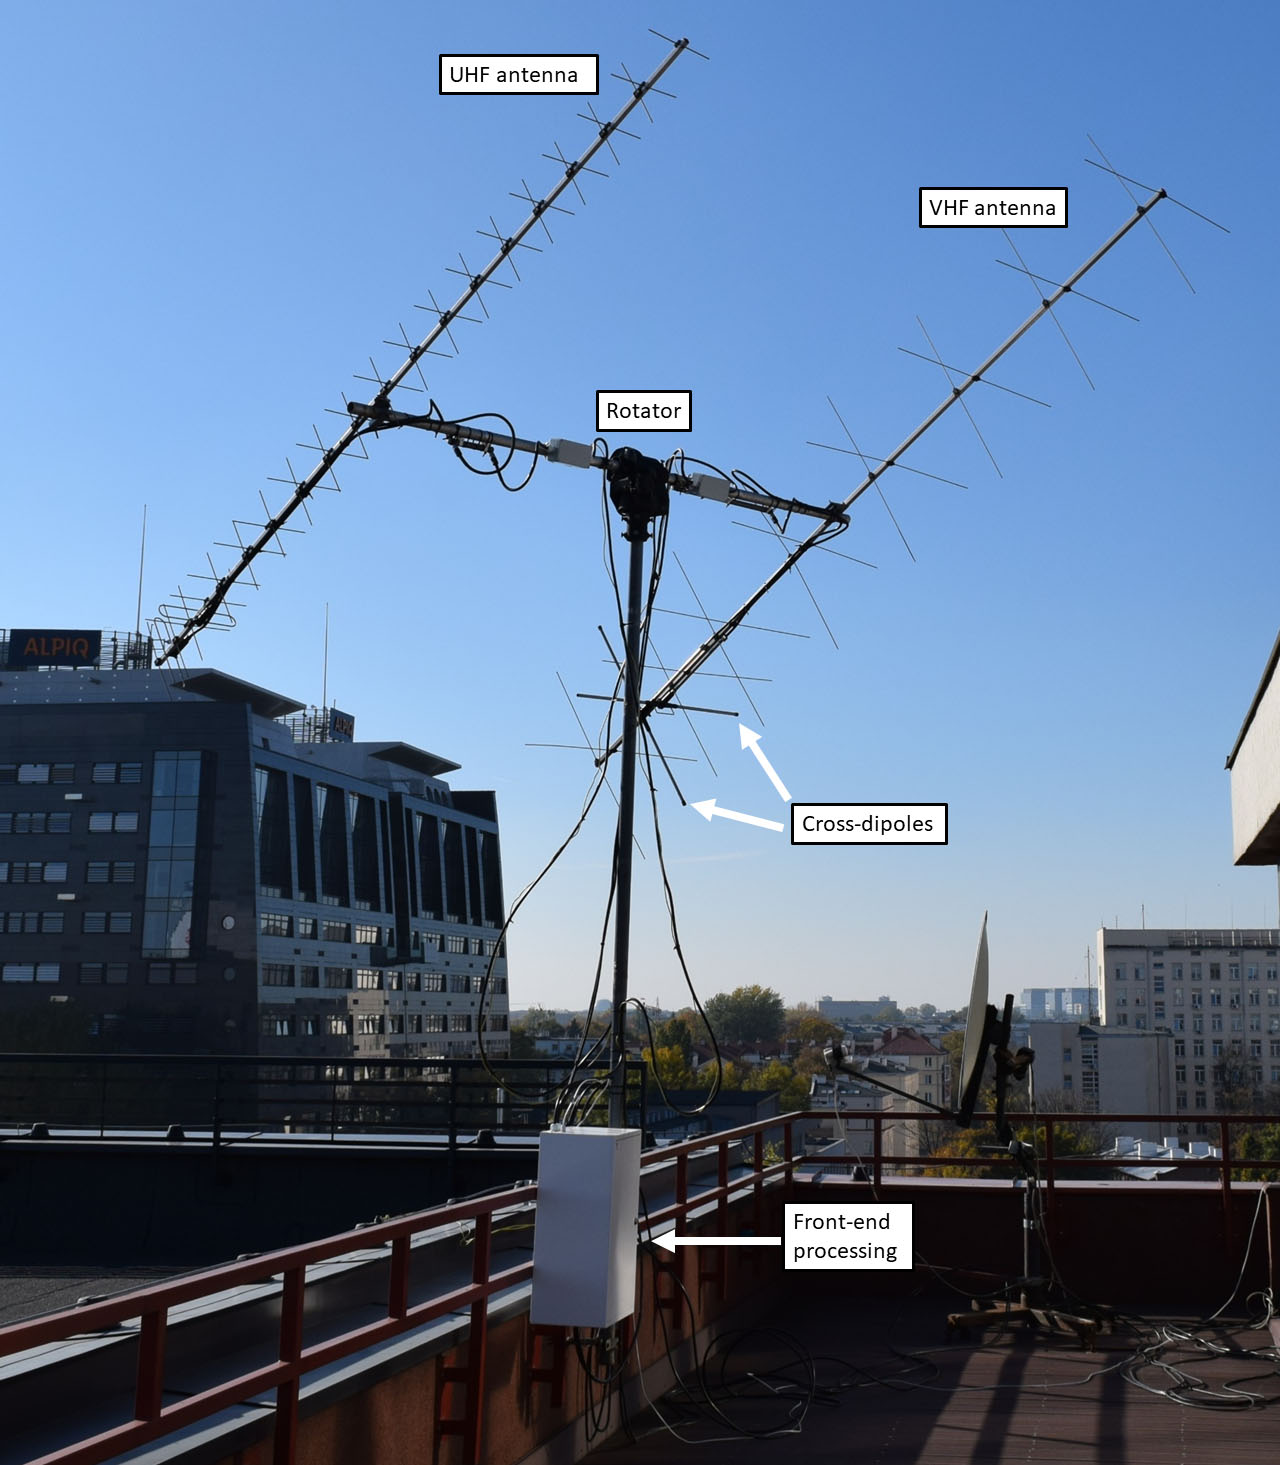
\includegraphics[width=0.5\paperwidth]{img/7/elka_antena_mast.jpg}
    \caption{Ground station picture}
    \label{elka_antena_mast}
\end{figure}

\begin{figure}
    \centering
    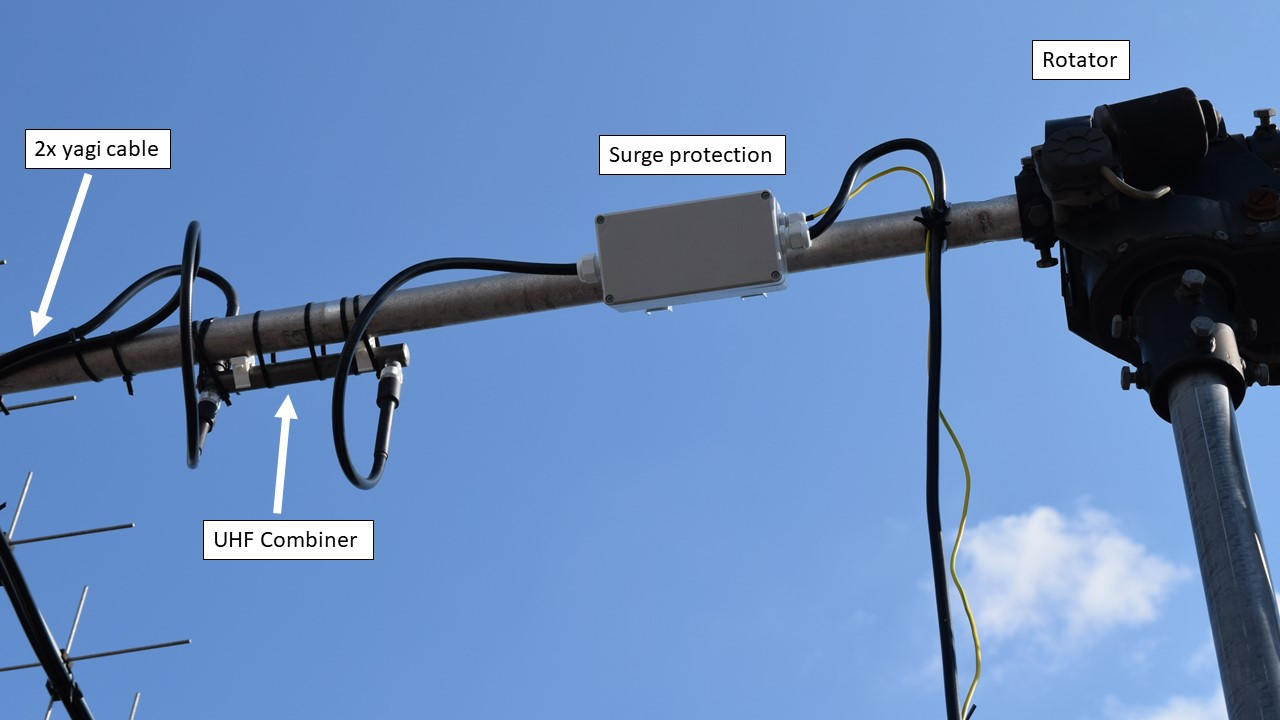
\includegraphics[width=0.75\paperwidth]{img/7/elka_antenna_rotator.jpg}
    \caption{Antenna rotator and boom}
    \label{elka_antenna_rotator}
\end{figure}

\begin{figure}
    \centering
    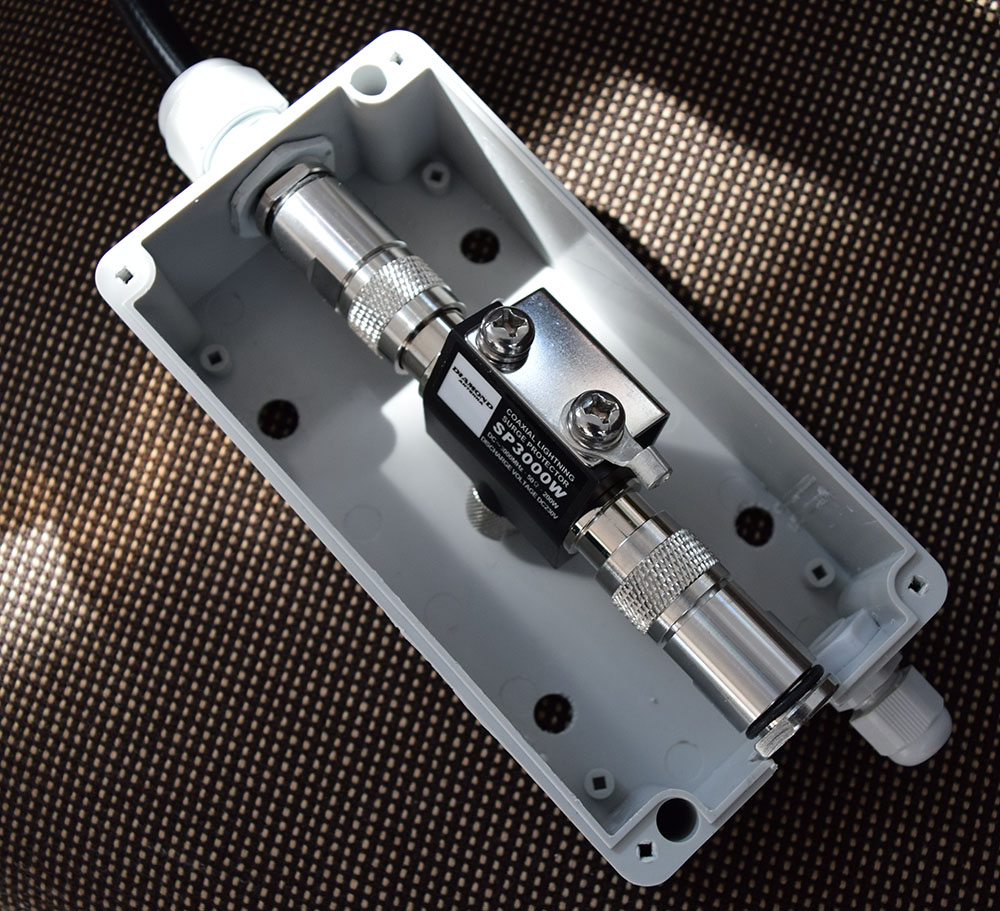
\includegraphics[width=0.5\paperwidth]{img/7/coax_surge_protection.jpg}
    \caption{Diamond SP3000W coaxial lightning surge protector}
    \label{coax_surge_protection}
\end{figure}



\section{Antennas}
PW-Sat2 is transmitting radio signals with linear polarization, nevertheless ground station  polarization should be circular, due to the random tumbling of the satellite. This will reduce the gain of the antennas, but the signal strength will be constant regardless of the satellite rotation. Cross-Yagi antennas were selected, and two linear planes antennas were phased with coaxial cable and symmetrical splitters/combiners. The diagram of the antenna phasing is shown in the figure \ref{antenna_phasing_diagram}. The length of the cables between the splitter/combiner and the dipoles should, with the dipole shift on the boom, create a \SI{90}{\degree} shift to create circular polarization. Two splitters/combiners were selected for antenna phasing: Tonna 31202 for VHF and Tonna 31270 for UHF.

\begin{figure}
    \centering
    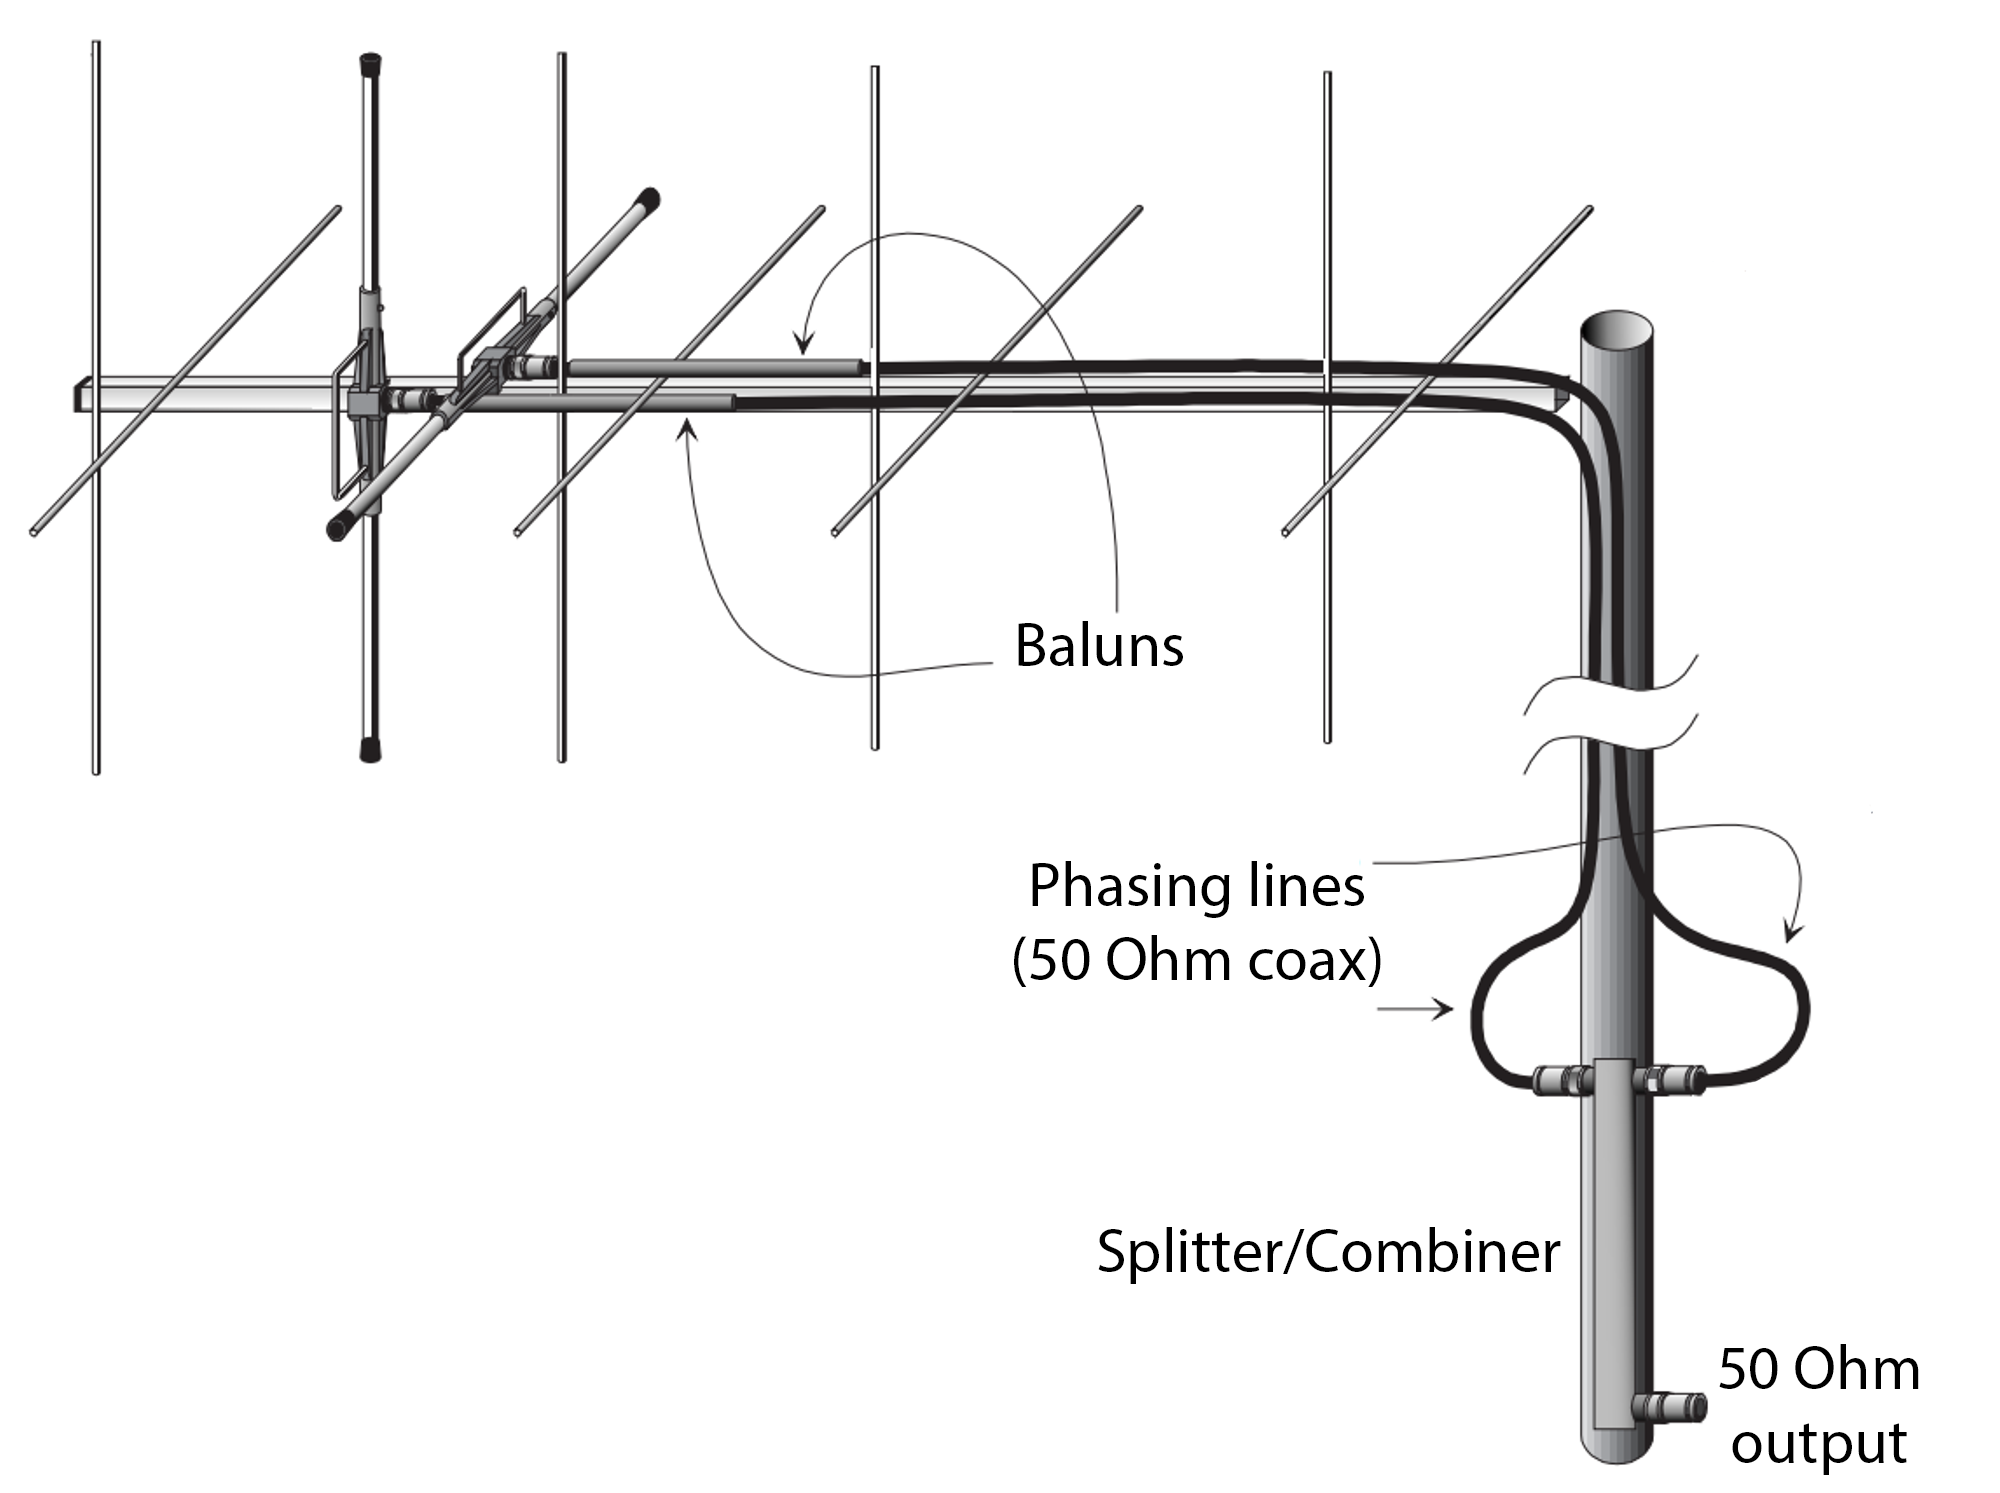
\includegraphics[width=0.5\paperwidth]{img/7/antenna_phasing_diagram.png}
    \caption{Antenna phasing}
    \label{antenna_phasing_diagram}
\end{figure}


Radiation patterns of the antennas are shown in the figures \ref{radiation_144} and \ref{radiation_435} as declared by the manufacturer. 

Antennas were selected to be the longest possible, limited by the antenna mast height. Selected antenna characteristics:

\begin{tabular}{c|c}
     \textbf{Downlink} & \textbf{Uplink} \\ \hline
     Tonna 220938 & Tonna 20818 \\
     UHF 2x 19 elements & VHF 2x 9 elements \\
     loop dipole & linear dipole \\
     \SI{16.2}{\dBi} gain & \SI{13.2}{\dBi} gain \\
     \SI{30}{\degree} beamwidth & \SI{40}{\degree} beamwidth
\end{tabular}

\begin{figure}
    \centering
    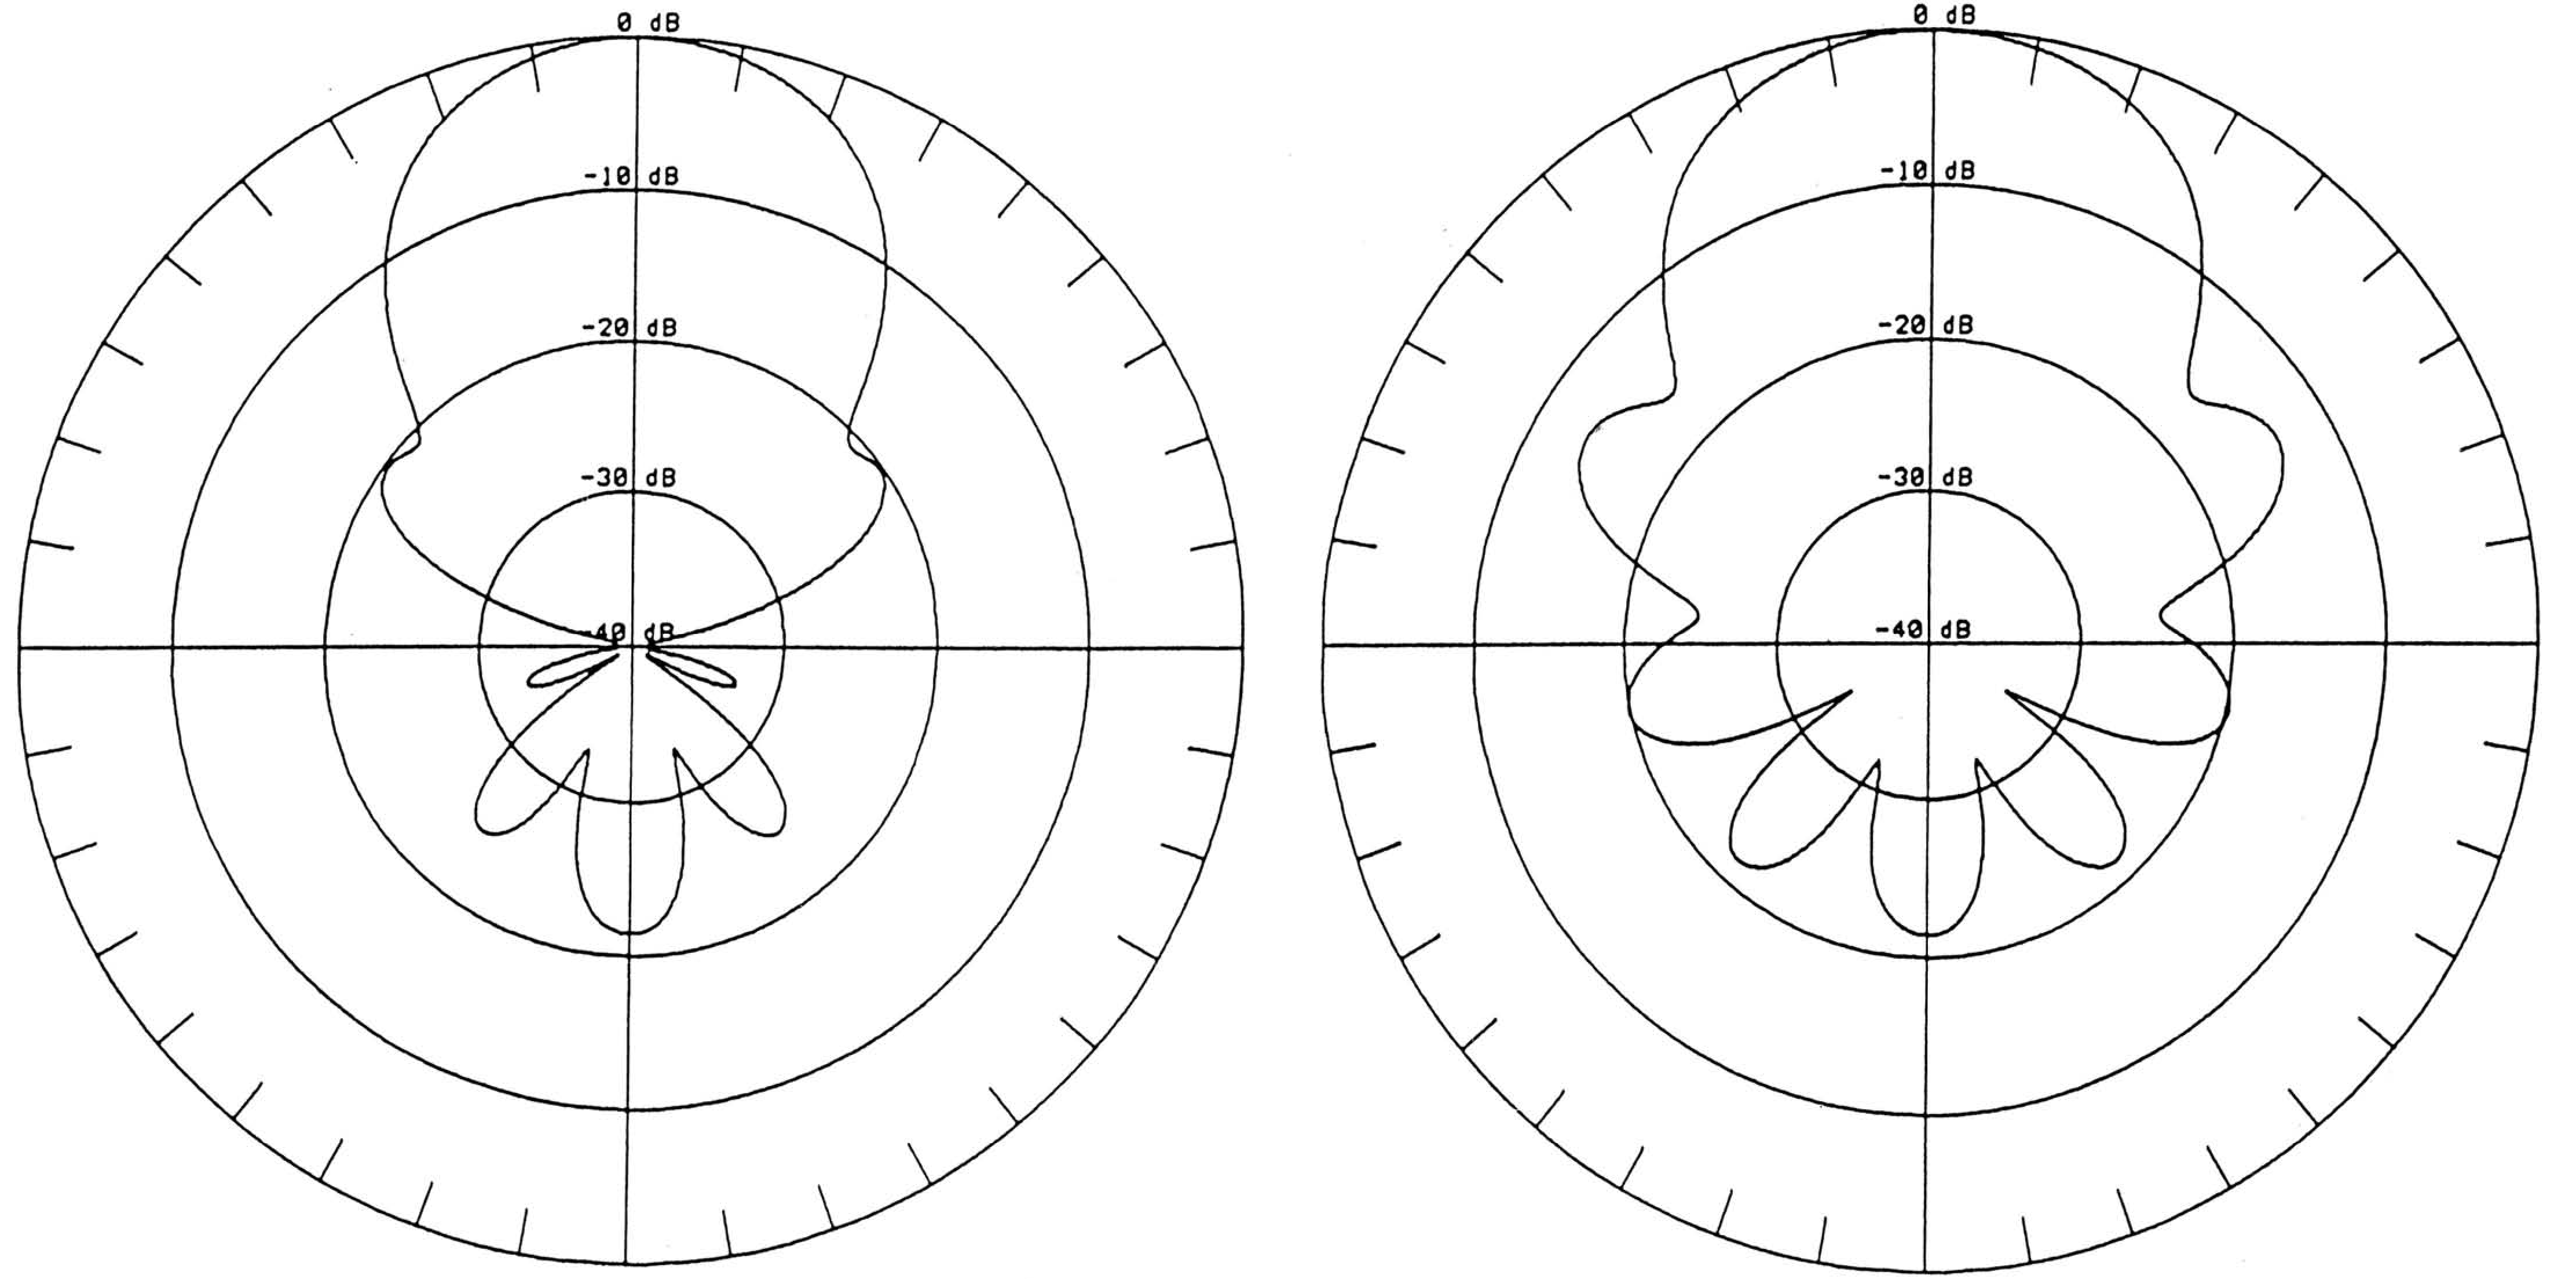
\includegraphics[width=0.75\paperwidth]{img/7/radiation_144.png}
    \caption{VHF antenna radiation pattern - E and H plane.}
    \label{radiation_144}
\end{figure}

\begin{figure}
    \centering
    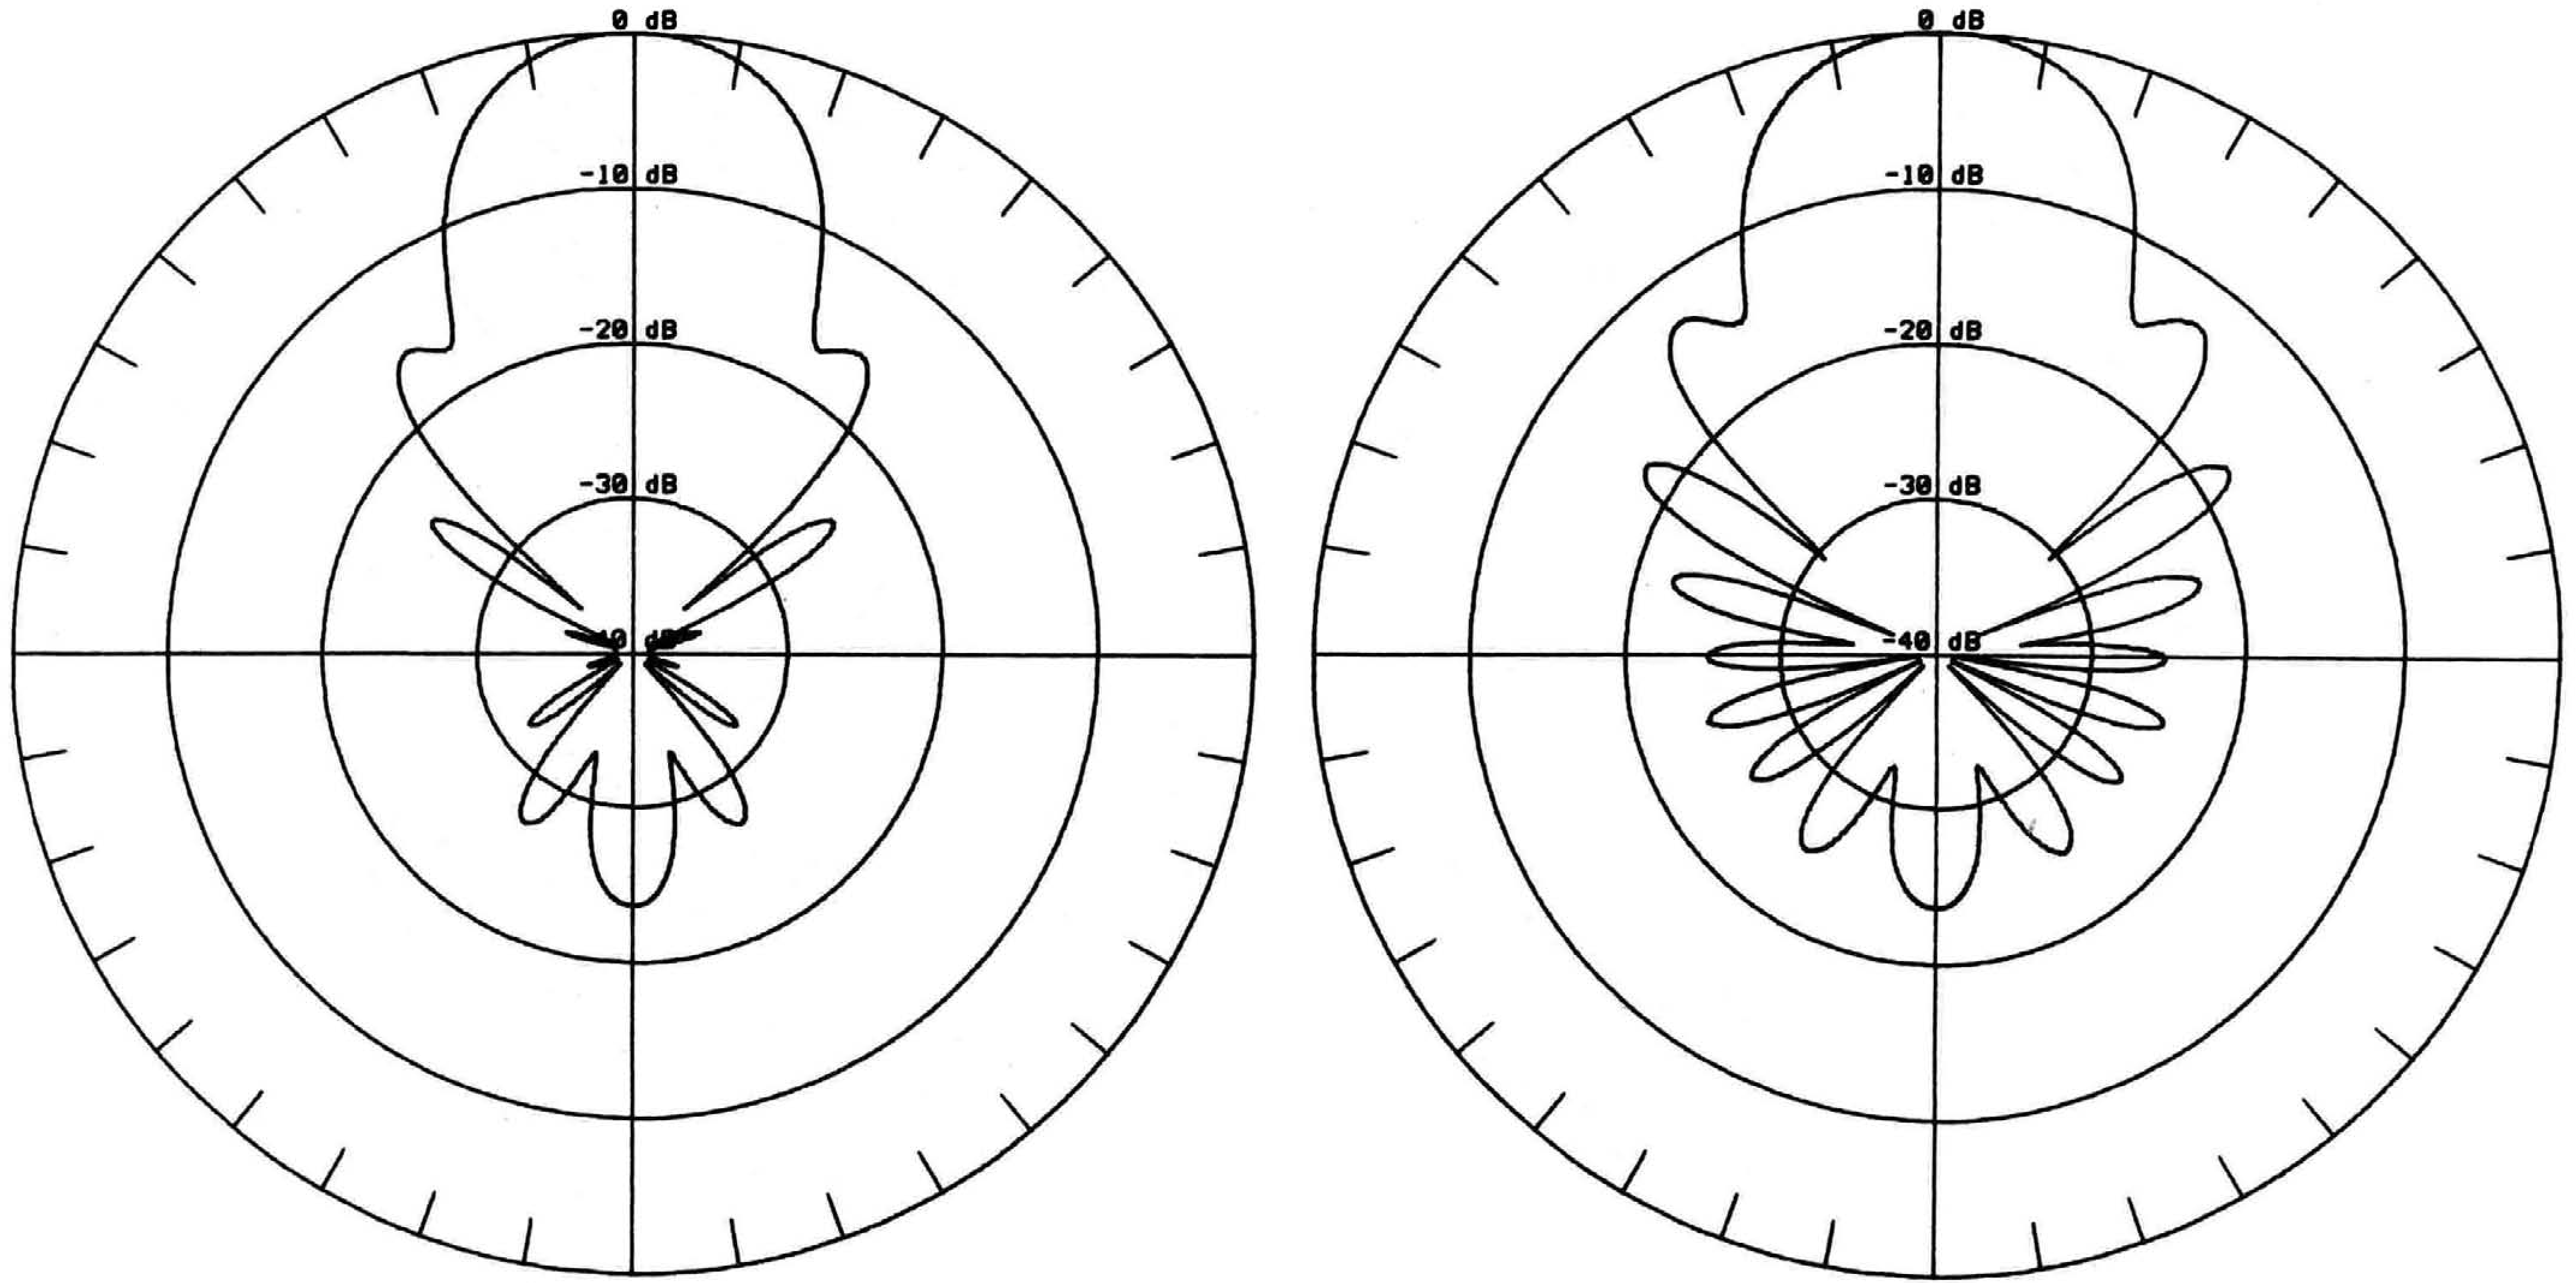
\includegraphics[width=0.75\paperwidth]{img/7/radiation_435.png}
    \caption{UHF antenna radiation pattern - E and H plane.}
    \label{radiation_435}
\end{figure}



\subsection{Splitters/combiners measurements}
Splitters/combiners were tested prior to its mounting. The most important parameters of the splitter is the insertion loss, amplitude and phase imbalance between the paths and the isolation of the splitter. All of the parameters were tested using Rohde \& Schwarz ZVL Vector Network Analyser, in the configurations shown in the figure \ref{splitter_measurement_diagram}. The results of the insertion loss (Fig. \ref{splitter_amplitude}) show that it is negligible - unmeasurable within tolerances of the VNA. Amplitude imbalance is also very good - much less than \SI{0.1}{\dB}. The phase imbalance is also very good for both splitters (Fig. \ref{splitter_phase}) - less than \SI{1}{\degree}. The isolation (Fig. \ref{splitter_isolation}) is the worst parameter of the measured splitters (only about \SI{6}{\dB}), but in the case when both antennas receive the same signal it is not an issue.

\begin{figure}
    \centering
    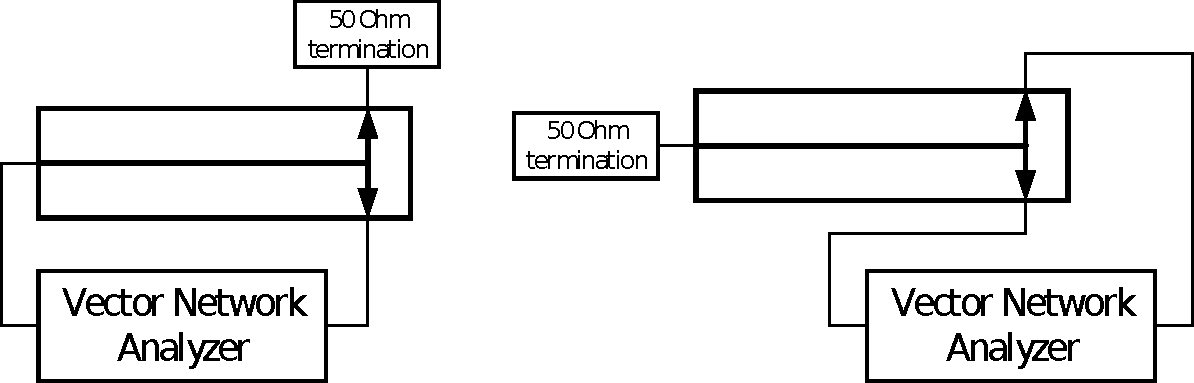
\includegraphics[width=0.75\paperwidth]{img/7/splitter_measurement_diagram.pdf}
    \caption{Splitter/combiner measurement block diagram for through and isolation measurement}
    \label{splitter_measurement_diagram}
\end{figure}

\begin{figure}
    \centering
    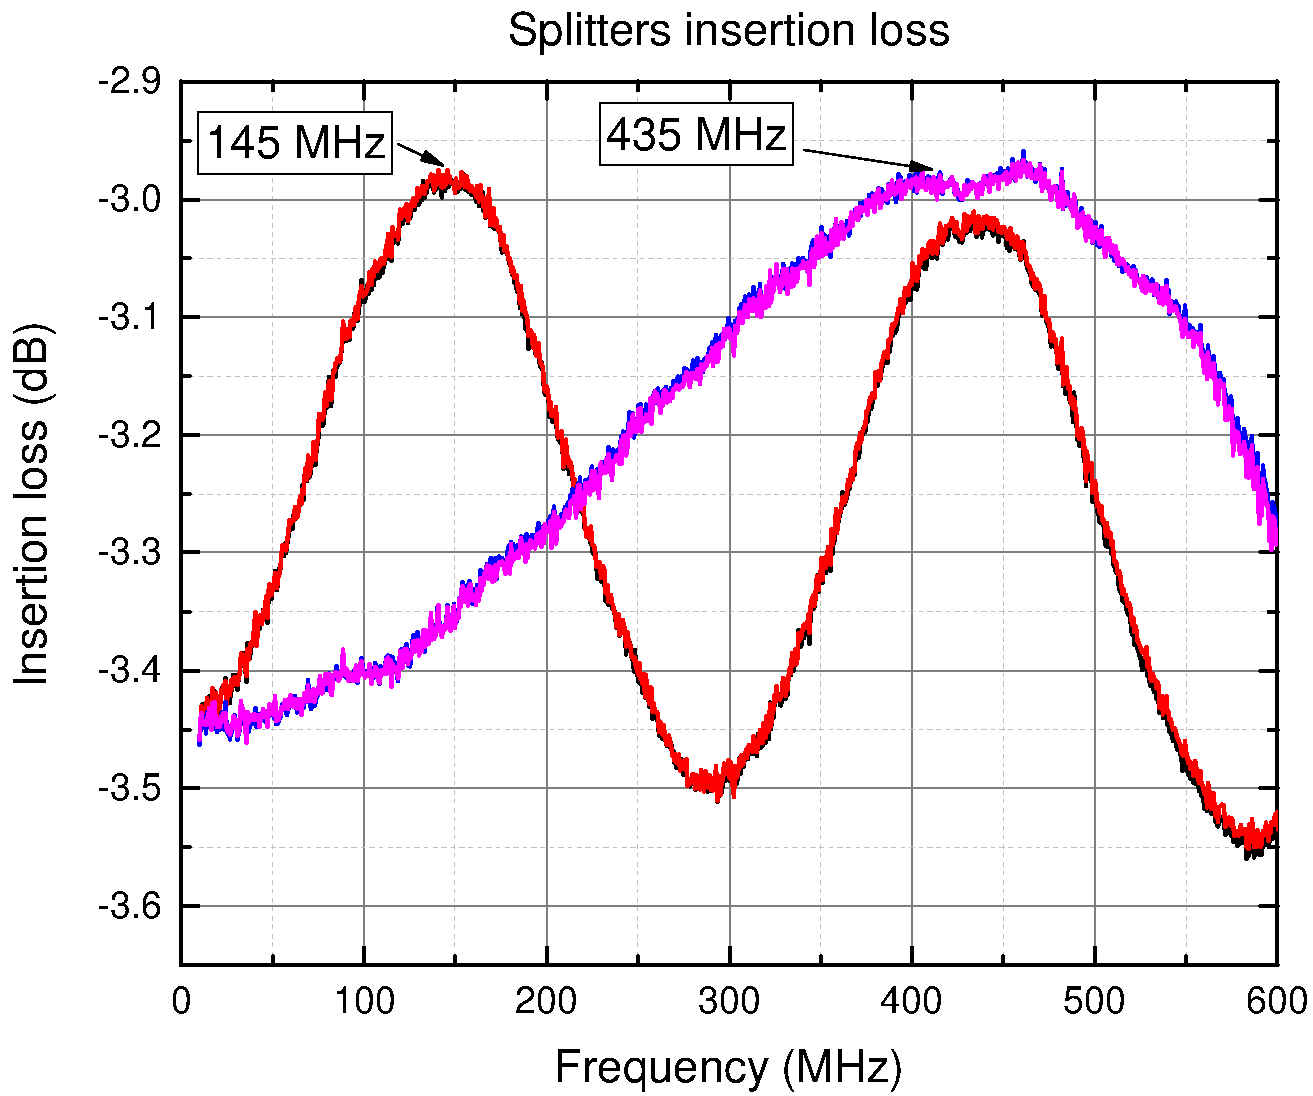
\includegraphics[width=0.6\paperwidth]{img/7/splitter_amplitude.pdf}
    \caption{Splitters/combiners insertion loss}
    \label{splitter_amplitude}
\end{figure}

\begin{figure}
    \centering
    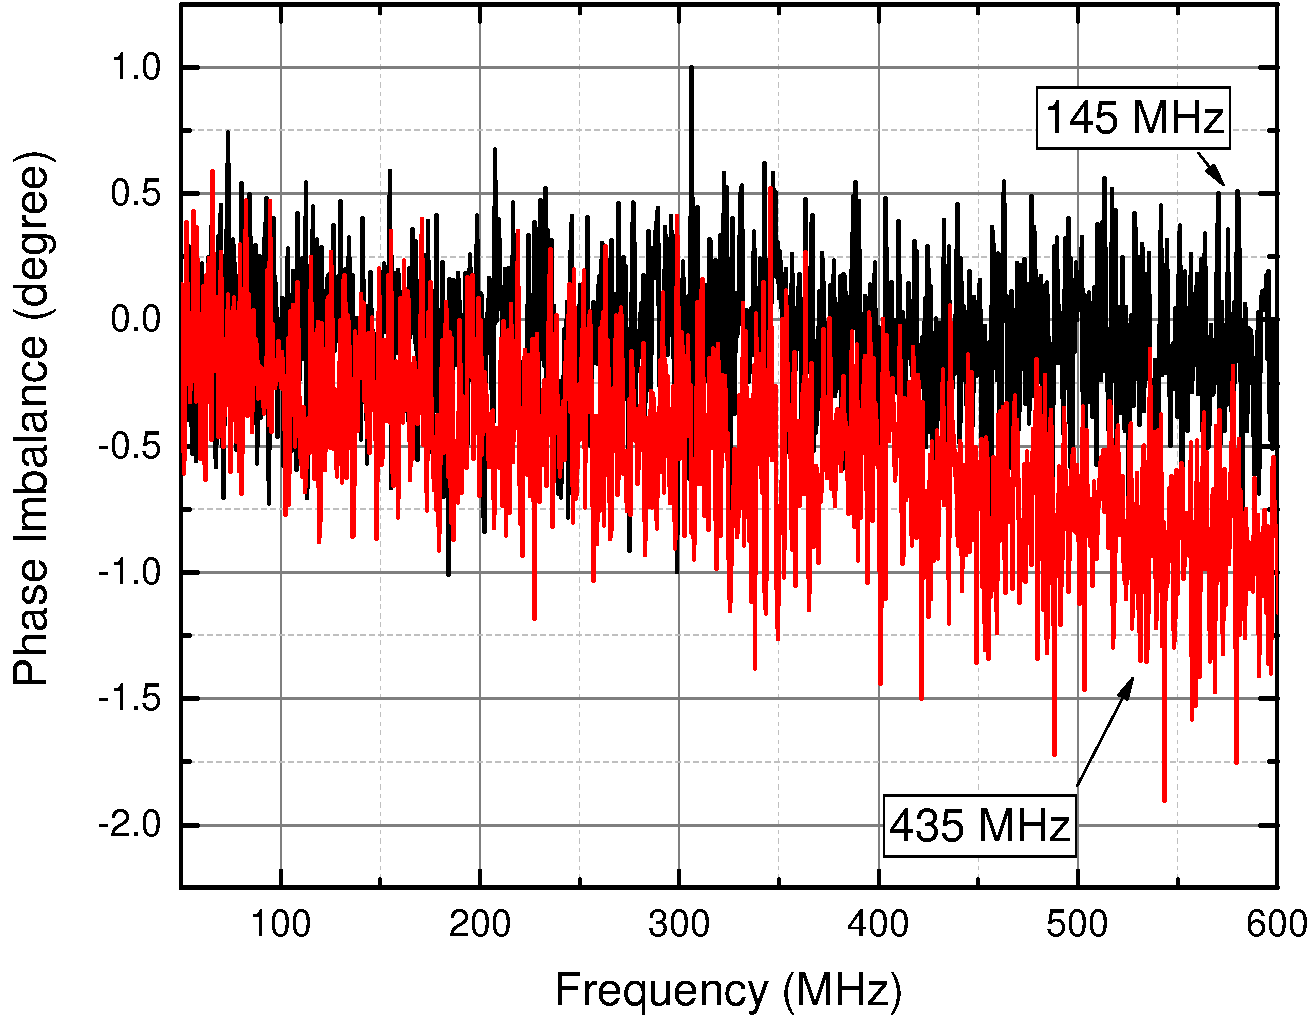
\includegraphics[width=0.6\paperwidth]{img/7/splitter_phase.pdf}
    \caption{Splitters/combiners phase shift imbalance}
    \label{splitter_phase}
\end{figure}

\begin{figure}
    \centering
    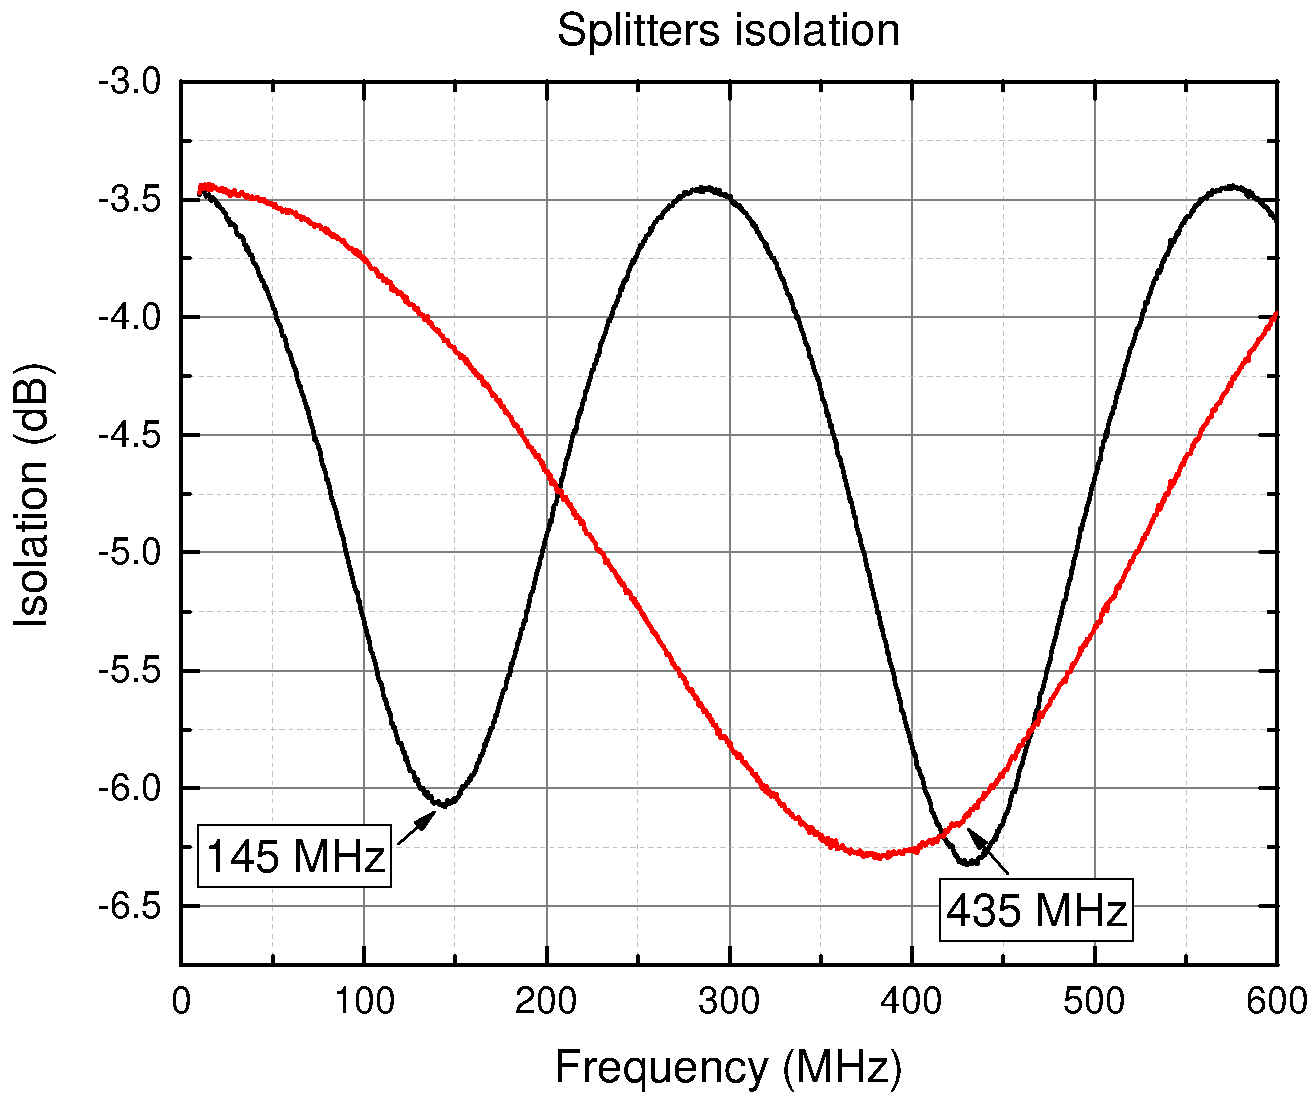
\includegraphics[width=0.6\paperwidth]{img/7/splitter_isolation.pdf}
    \caption{Splitters/combiners isolation}
    \label{splitter_isolation}
\end{figure}


% \subsection{Antenna Measurements}
% After the assembly, antennas were measured for their impedance matching and resonance. As the antennas are Yagi-Uda type, the most important element for matching is the dipole itself. Each antenna consist of two dipoles (with vertical and horizontal polarization) phased with a combiner. Measurements of the dipoles and the phased antenna were performed, and the result is shown in the table \ref{TODO}.

\newpage

\section{Uplink data flow}
Block diagram of uplink data chain is shown in the figure \ref{uplink_data_flow}. The telecommands issued by the operator are converted to the radio frames (\textbf{0}s and \textbf{1}s bits), later FSK modulated using GNUradio, finally to be FM-modulated, up-converted and power amplified by conventional voice transceiver.

\begin{figure}[H]
    \centering
    \includegraphics[width=0.6\paperwidth]{img/7/uplink_data_flow.eps}
    \caption{Uplink data flow}
    \label{uplink_data_flow}
\end{figure}

\section{Uplink baseband generation}
AFSK signal is generated by the GNURadio flowgraph shown in the figure \ref{uplink_flowgraph}. First, the telecommand is received by ZeroMQ slot, the packet is formatted and is is changed to the stream of bits. Each bit of the signal controls the frequency of the Voltage Controlled Oscillator (VCO) (\SI{1200}{\hertz} or \SI{2200}{\hertz} for \textbf{0} and \textbf{1}, respectively). During packet transmission, the transmit signal of the radio is enabled, and the audio signal is then generated by the audio card.

\begin{figure}
    \centering
    \includegraphics[width=0.8\paperwidth]{img/7/uplink_flowgraph.png}
    \caption{Uplink GNURadio companion flowchart}
    \label{uplink_flowgraph}
\end{figure}


\section{Uplink - transmitter}
Analog audio FM transceiver can be used to generate RF signal. The frequency deviation of the modulation was selected to allow to use radio amateur voice transceivers. Audio FSK signal (before FM-modulation) is generated by the software running on the PC. Radio is connected to the computer, which controls the audio to transmit and Push-To-Talk (PTT, transmission enable) signal.

During PW-Sat1 project, the Icom 910H amateur radio transceiver was used for both uplink and downlink, therefore it was proposed to use the the same radio as it do comply with all the requirements. Radio is shown in the figure \ref{Icom_910H_ref}. In case or need of larger output power the high-power amplifier can be connected to the output of the radio.

\begin{figure}[h]
    \centering
    \includegraphics[width=0.6\paperwidth]{img/7/icom910h.jpg}
    \caption{Icom 910H. Source: \cite{ICOM_910H_pic}}
    \label{Icom_910H_ref}
\end{figure}

Radio VHF FM transmit characteristics:

\begin{tabular}{c|c}
    Frequency & \si{144} - \SI{148}{\MHz} \\
    Frequency stability &  \SI{\pm 3}{\ppm} \\
    Output power & \SI{100}{\watt} \\
    Audio input & analog jack \\
    Audio bandwidth & \SI{4}{\kHz} \\
\end{tabular}

\newpage

\subsection{Standing Wave Ratio meter}
To check proper antenna connection and ensure long-term monitoring a SWR (Standing Wave Ratio) was installed. This instrument measures ratio of reflected power, thus providing information about antenna impedance matching. In case of antenna cracks or bending due to the high wind, any anomalies in the matching can be detected. SWR meter during the transmission is shown in the figure \ref{swr_meter_photo}, indicating that the VSWR of the antennas is lower than \si{1.05}. The output power is measured along the VSWR, and during the transmission it was equal to \SI{80}{\watt}.

\begin{figure}[H]
    \centering
    \includegraphics[width=0.5\paperwidth]{img/7/swr_meter_photo.jpg}
    \caption{Standing Wave Ratio meter during transmission}
    \label{swr_meter_photo}
\end{figure}

\subsection{Uplink watchdogs}
The spectrum and output modulation correctness in constantly monitored using so-called watchdog built using another Software Defined Radios (PlutoSDR, RTL-SDR) placed in the proximity of the main antennas.
By demodulating uplink signal and comparing it in the real time with transmitted frames the correctness of the transmission is guaranteed. Watchdog flowchart and graphical view are shown in the figure \ref{uplink_watchdog_flowgraph}.

\begin{figure}[H]
    \centering
    \includegraphics[width=0.8\paperwidth]{img/7/uplink_watchdog_flowgraph.png}
    \caption{Uplink watchdog GNURadio flowgraph}
    \label{uplink_watchdog_flowgraph}
\end{figure}

\newpage


% ------------------------------------------------------------
% ------------------------- DOWNLINK -------------------------
% ------------------------------------------------------------

\section{Downlink}
Receiving Signals from maximal slant range of about \SI{3000}{\kilo\meter} from a \SI{0.5}{\watt} transmitter requires very high processing gain and low noise factor of the system. System also needs to compensate for Doppler effect and ground interferences. The block diagram of the signal flow is shown in the figure \ref{downlink_diagram}.

\begin{figure}[H]
    \centering
    \includegraphics[width=0.8\paperwidth]{img/7/downlink_diagram.pdf}
    \caption{Downlink diagram}
    \label{downlink_diagram}
\end{figure}

\section{Signal front-end processing}
Radio front-end has two main purposes - to lower the system noise figure (by amplifying the signal with Low Noise Amplifier) and eliminate intermodulation with another signals (filtering). Its design consists of three stages: low loss cavity pass band filter, low noise amplifier and pass band SAW filter. Front-end signal processing is installed as close to the antenna as possible as shown in the figure \ref{elka_skrzynka}.

\begin{figure*}[h]
   \centering
\begin{tabular}{cc}
        \includegraphics[width=0.35\paperwidth]{img/7/elka_view.jpg}
    & 
        \includegraphics[width=0.35\paperwidth]{img/7/elka_skrzynka.jpg}
\end{tabular}
\label{elka_skrzynka}
\caption{PW-Sat2 ground station view and front-end processing.}
\end{figure*}

\subsection{Cavity filter}
Strong signals in the band of the amplifier can intermodulate in the receiver, resulting in variety of issues: from reduced gain to completely distorted signal of interest. Narrow-band cavity filter installed before the LNA to filter out out-of-band signals. Cavity filter due to its construction has very low insertion loss and regulated, narrow pass bandwidth in the cost of filter size and weight. Filter, shown in the figure \ref{cavity_filter_during_tuning} was tuned to the frequency of the PW-Sat2, with as narrow band as possible. After the tuning, the filter insertion loss is \SI{1.1}{\dB}, \SI{3}{\dB} bandwidth \SI{600}{\kHz} and \SI{20}{\dB} bandwidth - \SI{2}{\MHz}. Cavity filter has exceptionally good return loss - better than \SI{20}{\dB} in the passband. The insertion loss and return loss are shown in the figures \ref{cavity_filter_insertion_loss} and \ref{cavity_filter_return_loss}.

\begin{figure}
    \centering
    \includegraphics[width=0.5\paperwidth]{img/7/cavity_filter_during_tuning.jpg}
    \caption{Cavity filter during tuning}
    \label{cavity_filter_during_tuning}
\end{figure}

\begin{figure}
    \centering
    \includegraphics[width=0.5\paperwidth]{img/7/FilterLossG.pdf}
    \caption{Cavity filter insertion loss}
    \label{cavity_filter_insertion_loss}
\end{figure}

\begin{figure}
    \centering
    \includegraphics[width=0.5\paperwidth]{img/7/FilterMatchG.pdf}
    \caption{Cavity filter return loss}
    \label{cavity_filter_return_loss}
\end{figure}



\subsection{Low noise amplifier}
Low Noise Amplifier, installed close to the antenna reduces influence of the long cable attenuation between the antenna and the receiver and is designed to have low noise figure. According to the Friis formula, the total noise figure of the system will mostly depend on the insertion loss between the antenna and the noise figure of the Low Noise Amplifier. 

A dedicated Low Noise Amplifier was designed. As the main active component, a high-level Low Noise Amplifier: Mini-Circuits PGA-103+ \cite{lna_pga_datasheet} was used. Additional \SI{433}{\MHz} SAW filter was placed after the amplifier to reduce out of band harmonics and other unwanted products of amplification. Bias of the amplifier is created by RF Low Dropout Regulator Texas Instruments TPS7A47 \cite{lna_ldo_datasheet}. Amplifier was designed to support two-stage configuration, but for PW-Sat2 only first stage was populated. Schematic, PCB layout and the picture of the designed board are shown in the figures: \ref{lna_schematic} and \ref{lna_pcb}. The design is open source and all the source files can be found at \cite{lna_github}.

S-parameters of the LNA were tested using Rohde\& Schwarz ZVL Vector Network Analyser. Results are shown in the figures \ref{lna_gain} and \ref{lna_match}. Achieved single-stage gain: \SI{17.5}{\dB} with \SI{8}{\MHz} bandwidth.

\begin{landscape}
\begin{figure}
    \centering
    \includegraphics[width=1.12\paperwidth]{img/7/lna_schematic.pdf}
    \caption{Low Noise Amplifier Schematic}
    \label{lna_schematic}
\end{figure}
\end{landscape}

\begin{figure*}[h]
   \centering
\begin{tabular}{cc}
        \includegraphics[width=0.4\paperwidth]{img/7/lna_pcb.pdf}
    & 
        \includegraphics[width=0.3\paperwidth]{img/7/lna_assembled.jpg}
\end{tabular}
\label{lna_pcb}
\caption{Low Noise Amplifier PCB layout and assembled picture}
\end{figure*}
\begin{figure}[H]
    \centering
    \includegraphics[width=0.42\paperwidth]{img/7/LnaGain.pdf}
    \caption{Low Noise Amplifier gain}
    \label{lna_gain}
\end{figure}
\begin{figure}[H]
    \centering
    \includegraphics[width=0.42\paperwidth]{img/7/LnaMatch.pdf}
    \caption{Low Noise Amplifier return loss (input and output)}
    \label{lna_match}
\end{figure}

\subsection{Receiver}
Due to the custom packet format no commercially available integrated circuits were able to correctly receive packets, therefore a custom solution was required for de-modulation and packet recovery.
To receive BPSK signals, the phase recovery is necessary. One of the methods of the synchronous detection is the use of Costas loop \cite{costas_loop}. Most simple solution is to implement full signal chain: Costas loop, bit recovery and packet formatting using Digital Signal Processing on the baseband.

One of the possible and widely used methods is to use radio amateur transceiver in SSB mode - then radio acts as a multi-stage down-converter, allowing to receive baseband with audio card from PC. However, due to main purpose of transmitting audio signals, there is a lowpass filter for baseband at about \SI{3}{\kHz}. Using SSB mode for receiving PW-Sat2 is possible, however only for \SI{1.2}{\kbps} bitrate.

Another method was to use Software-Defined Radio, performing IQ downconversion and data transmission. The Radio Amateur Satellite Corporation designed an SDR receiver for their mission FUNcube Satellite. After mission success, they released their design and started selling FUNcube dongle shown in the figure \ref{funcube_pic}. Given that is was designed specifically for satellite communication and it was tested using similar CubeSat design, it was selected as the main receiver for PW-Sat2.

\begin{figure}[H]
    \centering
    \includegraphics[width=0.6\paperwidth]{img/4/funcube.jpg}
    \caption{FUNcube Dongle Pro+. Source: \cite{funcube}}
    \label{funcube_pic}
\end{figure}

The receiver  functionalities:
\begin{itemize}
    \item Doppler correction,
    \item IQ data recording,
    \item BPSK demodulation,
    \item bit recovery,
    \item packet formatting,
    \item multiple bitrate simultaneous decoders,
    \item sending data on-line to the operators,
    \item work with different Software-Defined Radios and SSB transceivers
\end{itemize}

The block diagram of the designed system is shown in the figure \ref{demodulator_block_diagram}. All of the signal processing blocks were created using GNUradio framework.

\begin{figure}[H]
    \centering
    \includegraphics[width=0.6\paperwidth]{img/7/demodulator_block_diagram.pdf}
    \caption{Demodulator Block Diagram}
    \label{demodulator_block_diagram}
\end{figure}

First stage, the SDR / transceiver can be any type of Software-Defined radio working with osmocom device drivers, FUNcube SDR or analog SSB radio using audio card. To mitigate the DC-offset and IQ imbalance, the output of this block is on non-zero IF - the frequency of the PW-Sat2 is shifted from the LO frequency. For SSB transceiver, it has to be tuned \SI{2}{\kHz} below the center frequency due to the limited bandwidth of the audio filters, and for the SDR transceiver to eliminate the DC peak effect, the signal is shifted by 1/4 of the bandwidth. Signal source dialog of the main application is shown in the figure \ref{gs_source_selection}.

\begin{figure}[H]
    \centering
    \includegraphics[width=0.6\paperwidth]{img/7/gs_source_selection.png}
    \caption{Ground station application - signal source selection}
    \label{gs_source_selection}
\end{figure}

Doppler correction is build on quadrature mixer and create zero-IF signal for the next processing blocks. Gpredict calculates required frequency shift and sends it to the block via TCP/IP connection. This updates local VCO frequency for the down-conversion. Latter, the signal is fist-stage filtered and saved to the file for logging purposes. GNUradio block diagram is shown in the figure \ref{gs_doppler_gnuradio}.

\begin{figure}[H]
    \centering
    \includegraphics[width=0.7\paperwidth]{img/7/gs_doppler_gnuradio.png}
    \caption{Doppler correction block GNUradio flowgraph}
    \label{gs_doppler_gnuradio}
\end{figure}

In the system, there are two demodulators (for \SI{1.2}{\kbps} and \SI{9.6}{\kbps} bitrates) operating simulateneously. This allows immediate signal reception during bitrate change by the operator without any manual intervention in the software. This was achieved using GNURadio "hierarchial blocks". Top demodulator block is shown in the figure \ref{gs_demodulator_hier}, and each of Downlink blocks (Fig. \ref{gs_demodulator_diagram}) is a complete demodulator. The demodulator has its own GUI to show user the status of the block (carrier lock, bit lock, constellation diagram), shown the figure \ref{gs_demodulator_gui}.
Downlink receiver does the following operations:
\begin{itemize}
    \item resampling - to create a demodulator with selectable bitrate each of the bitrate decimates the input signal accordingly,
    \item Automatic Gain Control - the power of the signal should be constant as the tuning constants are dependent on the signal amplitude,
    \item Costas loop - carrier recovery and phase demodulation,
    \item filtering - low-pass signal with matched Root Raised Cosine filter to eliminate out of band noise and minimize Inter Symbol Interference,
    \item Symbol synchronization - recovers bits from the baseband signal,
    \item packet framing - builds a frame from stream of bits,
    \item frame pass to the higher level software.
\end{itemize}

\begin{figure}[H]
    \centering
    \includegraphics[width=0.7\paperwidth]{img/7/gs_downlink_hier.png}
    \caption{Hierarchial receiver GNUradio flowgraph}
    \label{gs_demodulator_hier}
\end{figure}

\begin{figure}[H]
    \centering
    \includegraphics[width=0.7\paperwidth]{img/7/gs_demodulator_diagram.png}
    \caption{Ground station demodulator GNUradio flowgraph}
    \label{gs_demodulator_diagram}
\end{figure}

\begin{figure}[H]
    \centering
    \includegraphics[width=0.7\paperwidth]{img/7/gs_demodulator_gui.jpg}
    \caption{Ground station demodulator GUI}
    \label{gs_demodulator_gui}
\end{figure}

After the packet reception, it is shown for the user (as in the figure \ref{gs_frame_view}) and uploaded to the cloud for further analysis by the operations team.

\begin{figure}[H]
    \centering
    \includegraphics[width=0.6\paperwidth]{img/7/gs_frame_view.png}
    \caption{Ground station received frame view}
    \label{gs_frame_view}
\end{figure}


\subsubsection{Measurements}
%Frequency correction block was tested using already flying satellites, verifying stability of frequency after correction.
The test setup for evaluating demodulator performance is shown in the figure \ref{sensitivity_test_diagram}, and consist of:
\begin{itemize}
    \item PlutoSDR - transmitter of the frames with regulated center frequency and output power,
    \item \SI{60}{\dB} attenuator,
    \item Funcube Pro+ SDR with LNA and cavity filter - full receiver used in the ground station
\end{itemize}

\begin{figure}
    \centering
    \includegraphics[width=0.8\paperwidth]{img/7/sensitivity_test_diagram.pdf}
    \caption{Sensitivity test measurement setup}
    \label{sensitivity_test_diagram}
\end{figure}

Frames to be transmitted were recorded with Software-Defined Radio during flatsat test campaign and replayed during sensitivity tests. This ensures that all the important inadequacies transmitted by the radio transmitter were also taken into account. With the test setup, sensitivity was automatically measured by varying output power of the transmitter (in \SI{1}{\dB} steps) and PER was recorded for each point. During the process, different parameters of the demodulator were tuned to increase the sensitivity, and the sensitivity was tested for different bitrates as well.

The Costas loop performance and bit sync clock recovery blocks were tested first. The main parameter of the blocks are the bandwidths of the Phase Locked Loops inside them. During the test, input power to the receiver was set to \SI{3}{\dB} above the sensitivity level. The parameters were automatically adjusted and the graphs \ref{sensitivity_costas} and \ref{sensitivity_bitsync} show the number of decoded frames in the function of the parameter. For Costas loop there is a significant maximum, when the bandwidth is wide enough to "catch" sync during the preamble and not lose sync during noisy transition. Changing a loop bandwidth of the symbol sync block does not affect the number of frames significantly, as the clock frequencies are relatively slow and stable.

\begin{figure}[H]
    \centering
    \includegraphics[width=0.6\paperwidth]{img/7/costasG.pdf}
    \caption{Costas loop tuning}
    \label{sensitivity_costas}
\end{figure}

\begin{figure}[H]
    \centering
    \includegraphics[width=0.6\paperwidth]{img/7/symbolsyncG.pdf}
    \caption{Symbol synchronization tuning}
    \label{sensitivity_bitsync}
\end{figure}


The sensitivity as the number of received frames vs input power was also measured, for every receiver bitrate (\si{1200}, \si{2400}, \si{4800} and \SI{9600}{\bps}). The results (fig. \ref{sensitivity_tests}) show that for every doubling the bitrate the sensitivity decreases by \SI{3}{\dB}. Is is according to the theory, because doubling the bitrate doubles the noise bandwidth and reduces energy per bit by factor of two. The model of the BPSK receiver also is similar to the gathered data (fig. \ref{sensitivity_test_model}). The final sensitivity is \SI{-127}{\dBm} for \SI{1200}{\bps} and decreases by \SI{3}{\dB} for every doubling the bitrate (\SI{-118}{\dBm} for \SI{9600}{\bps}).

\begin{figure}
    \centering
    \includegraphics[width=0.6\paperwidth]{img/7/sensitivityMG.pdf}
    \caption{Costas loop tuning}
    \label{sensitivity_tests}
\end{figure}

\begin{figure}
    \centering
    \includegraphics[width=0.6\paperwidth]{img/7/sensitivityG.pdf}
    \caption{Symbol synchronization tuning}
    \label{sensitivity_test_model}
\end{figure}
\chapter{Link budget}
The link budget was calculated to estimate the link status, whether the selected components are sufficient to "close" the link – to maintain the communication with the required Packet Error Rate. A link budget calculates all the gains and losses in the radio system, estimating the link margin. In the satellite case, a link budget is a valuable tool - because of the direct line of sight between two communicating nodes, most of the parameters are well known and stable throughout the system lifetime. Main gains from the system come from: output power of the transmitter and the antennas gain, whereas losses include: free space loss, losses through the medium (atmospheric losses, ionization losses), cable and other in-line devices attenuation, polarisation losses and antenna pointing losses. This section describes the PW-Sat2 link budget, which was based on the AMSAT/IARU Link Budget \cite{amsat_link_budget}.

\section{Orbit and slant range}
A slant range (fig \ref{slant_range}) is a maximal distance between the spacecraft and the ground station. It is calculated from the Orbit altitude and the minimal elevation required. For PW-Sat2, useful elevation was assumed at \SI{5}{\degree}. Assumed orbital parameters gives maximum slant range of about \SI{2300}{\kilo\meter} (fig. \ref{slant_range_calc}) and period of \SI{96}{\minute}.

\begin{figure}
    \centering
    \includegraphics[width=0.8\paperwidth]{img/8/slant_range.pdf}
    \caption{Slant range. Source: \cite{amsat_link_budget}}
    \label{slant_range}
\end{figure}

\begin{figure}
    \centering
    \includegraphics[width=0.8\paperwidth]{img/8/slant_range_calc.pdf}
    \caption{Slant range calculation.}
    \label{slant_range_calc}
\end{figure}

\section{Transmitter capabilities}
The transmitter output power and any in-line losses, as well as antenna mismatch,  are entered and calculated in the link budget. All the in-line losses are estimated, such as the feeder loss, splitter insertion loss and, if applicable, any other elements, such as the surge protection. The result is the power that is actually delivered to the antennas on both the ground station and the spacecraft. The results shown in the figures \ref{link:tx_gs} and \ref{link:tx_spacecraft} indicate the output power \SI{26.63}{\dBm} on the spacecraft and \SI{47.45}{\dBm} on the ground station.

\begin{figure}
    \centering
    \includegraphics[width=0.8\paperwidth]{img/8/tx_gs.pdf}
    \caption{Ground station output power calculation}
    \label{link:tx_gs}
\end{figure}

\begin{figure}
    \centering
    \includegraphics[width=0.8\paperwidth]{img/8/tx_spacecraft.pdf}
    \caption{Spacecraft output power calculation}
    \label{link:tx_spacecraft}
\end{figure}


\section{Antenna gain}
The antenna gain directly affect the radio link budget. The directional gain of the antennas is taken from the documentation of the manufacturers and for the antennas in the system they are equal to:
\begin{itemize}
    \item Ground station - Cross-Yagi antennas, \SI{13.2}{\dBi} for uplink, \SI{16.2}{\dBi} for downlink,
    \item Spacecraft - both antennas are dipoles, \SI{2.15}{\dBi} as for ideal dipole is assumed as the antennas are working in the resonance. 
\end{itemize}


\section{Medium losses}
The main signal loss in the spacecraft communication comes from the Free space loss, given by the formula: 
$$\text{Loss [dB]} = 22 + 20 \cdot \log_{10} (\text{d}/\lambda) \text{~~~~where $d$ - distance in meters, $\lambda$ - wavelength}$$ Other sources of losses taken into the consideration for the sub-GHz bands are atmospheric losses and losses in the ionosphere. Atmospheric absorption strongly depends on the total number of molecules along the path between the spacecraft and the ground station - therefore the elevation angle. Losses due to the atmospheric gases are nearly independent of atmospheric temperature, density and relative humidity at frequencies below 2 GHz. \cite{sat_propagation}. At \SI{5}{\degree} elevation, the atmospheric are estimated at \SI{2.1}{\dB}. The ionosphere limits the lowest frequency at which satellite communications is possible. Below \SI{20}{\MHz}, during solar maximum, signals are usually fully absorbed or reflected by the layers of the ionosphere. VHF, UHF and Microwave frequencies are influenced far less amount, but the value of the attenuation varies with time. For the purpose of the calculation above \SI{100}{\MHz}, is sufficient to estimate losses in the ionosphere as lower than \SI{1}{\dB}.

\vspace{0.5cm}
Total medium losses are equal:
\begin{itemize}
    \item Uplink - \SI{145.9}{\MHz} - $\text{Loss} = \SI{146.2}{\dB}$
    \item Downlink - \SI{145.9}{\MHz} - $\text{Loss} = \SI{155.7}{\dB}$
\end{itemize}


\section{Polarization losses}
On the ground station, both antennas have circular polarization, whereas, on the spacecraft, antennas are linearly polarized. This eliminates the effect of signal strength variance with the rotation of the satellite, but only the half power is received by the antennas. The polarization loss of \SI{3}{\dB} was assumed in both uplink and downlink.

\section{Antenna pointing losses}
Antenna pointing losses are exhibited when the maximal directivity gain of the antennas are not aligned with the receiver (fig. \ref{link:pointing_loss}). For ground station, the rotator and its controller are pointing with the accuracy of about \SI{1}{\degree}, but due to the wind and other non-ideal factors, the pointing error was assumed for \SI{5}{\degree}. The antenna gain loss was read from the radiation patterns (fig. \ref{radiation_144} and \ref{radiation_435}) and estimated at \SI{1}{\dB}. For the spacecraft, as the antennas have dipole characteristics, they are mostly omnidirectional, but with significant drops in the directivity along the dipole axis. The communication will break at some angles along the dipole axis; it was assumed that the coverage of \si{300} per \SI{360}{\degree} is sufficient. At standard dipole roll-off factor (fig. \ref{link:dipole_pattern}), \SI{70}{\degree} pointing error equals to \SI{4.7}{\dB} pointing loss.

\begin{figure}
    \centering
    \includegraphics[width=0.5\paperwidth]{img/8/pointing_loss.pdf}
    \caption{Pointing losses. Source: \cite{amsat_link_budget}}
    \label{link:pointing_loss}
\end{figure}

\begin{figure}
    \centering
    \includegraphics[width=0.4\paperwidth]{img/8/dipole_pattern.pdf}
    \caption{Dipole antenna radiation pattern. Source: \cite{amsat_link_budget}}
    \label{link:dipole_pattern}
\end{figure}


\section{Antenna temperature}
For receiver antennas, the antenna temperature is the total noise figure added by the antenna which comes from other sources than a transmitter of interest. It adds to the noise produced by the Low Noise Amplifier, resulting in lowering the Signal To Noise ratio.
The sky temperature, as seen by a spacecraft, must be viewed from its perspective. In the beamwidth of the omnidirectional antenna on Low Earth Orbit, there is a half of a sphere of the deep space and half of the Earth. The sky itself which is nominally at \SI{2.7}{\kelvin} but, at frequencies below \SI{2}{\GHz}, antenna noise also includes galactic noise, which is highest in directions that intercept the disk of the Milky Way.  At \SI{146}{\MHz} this value can be as high as \SI{1700}{\kelvin} and as low as \SI{80}{\kelvin} \cite{amsat_link_budget}. The average Earth temperature used is \SI{290}{\kelvin}. However, the Earth may be warmer due to man-made noise sources that can be distributed on the surface of the planet. The average antenna temperature of the spacecraft was assumed to $0.5 \cdot \SI{70}{\kelvin} + 0.5 \cdot \SI{330}{\kelvin} = \SI{200}{\kelvin}$.
For a ground station antenna, the Sky Temperature value must include not only the noise intercepted by the ground station antenna coming from the colder sky into which the antenna is looking but, it has to include any terrestrially generated noise that may be generated in the proximity of the station. This condition is worst when the ground station antenna is at low elevation angles and pointed in the direction of the source of the noise. For PW-Sat2, the receiver antenna is placed in the middle of the Warsaw, resulting in increased temperature depending on the azimuth of the antenna. During ground station calibration, the power spectrum density was measured using the spectrum analyzer, resulting in the noise floor of about \SI{-132}{\dBm} in \SI{10}{\kHz} RBW. This implies the antenna temperature of about \SI{500}{\kelvin}.

\section{Receiver performance}
The receiver performance was measured for both uplink and downlink using the attenuators and packet transmitters. During the sensitivity tests, the "effective" antenna temperature was \SI{290}{\kelvin} - the noise was produced by the electrical components in the room temperature. This means that during the mission, the sensitivity will be affected by the noise added by the antenna.
For uplink, the effective sky antenna (\SI{200}{\kelvin}) is actually lower then the room temperature, meaning that the sensitivity of the system will improve by $10\cdot \log_{10}(200/290) = \SI{1.6}{\dB}$, resulting in receiver sensitivity for \SI{1}{\percent} PER: \SI{-98}{\dBm}.
In the ground station, the effective antenna temperature will be higher than during tests on the bench, resulting in the reduction of the sensitivity by $\SI{2.3}{\dB}$. This gives the effective sensitivity at \SI{-124}{\dBm}.

\section{Link budget summary}
Summing all the gains and losses produces a valuable overview of the system performance (fig. \ref{link:link_status}). The power on the receiver ports of the system is calculated and compared to the sensitivities of the receivers, resulting in link status and margin. The link margins are above \SI{5}{\dB} - the safe limit and are equal to \SI{6.0}{\dB} for downlink and \SI{5.7}{\dB} for uplink. Most of the time, the performance will be better due to the lower pointing losses of the spacecraft. 

\begin{figure}
    \centering
    \includegraphics[width=0.8\paperwidth]{img/8/link_summary.pdf}
    \caption{System performance summary}
    \label{link:link_status}
\end{figure}
\chapter{Mission results}
% During the project, all of the radio system parts have been chosen, measured and verified. The satellite, consisting of the the communication module and the folded antennas was integrated. Ground station was build using off-the-shelf radio transceiver with custom designed Low Noise Amplifier.
% The measurement of the sensitivity of the receivers were performed.
% Link budget was calulated to make sure that the link margins are sufficient, using the measured data.

\section{Primary mission}
At $3^{rd}$ of December 2018, PW-Sat2 was launched on \SI{590}{\kilo\meter} orbit on-board Falcon9 rocket from SpaceX company. During first hours after launch, PW-Sat2 was inside the deployer, completely turned off by the hardware kill-switch. 4 hours after the launch, it was deployed and the system turned on automatically. On-Board software, after silent period of \SI{40}{\minute} performed antenna deployment procedure and started transmitting beacon data every \SI{60}{\second}. First beacon frame (consisting of satellite telemetry) was received by Scott Chapman (K4KDR) from United States of America at 6:10 am the day after launch. 

During the first couple of days of orbital operations the Bus and Payload commissionings were performed by the operators on the ground. At first, satellite was transmitting with \SI{1200}{\bps} downlink speed, providing reliable radio link. When the basic satellite data was verified, communication module was switched to \SI{9600}{\bps} to speed up data transfer and reduce power consumption. PW-Sat2 took first polish satellite photograph and transferred in to the ground stations at $5^{th}$ of December 2018 (fig. \ref{sat_photo}). It was taken by a part of camera built-in tests and downloaded on request from ground.

\begin{figure}[H]
    \centering
    \includegraphics[width=0.5\paperwidth]{img/9/sat_photo.jpg}
    \caption{First polish satellite photo, taken of $5^{th}$ of Decemer 2018}
    \label{sat_photo}
\end{figure}

During the launch, \si{64} satellites were launched together and were separated from the upper stage of the rocket by spring actions. At first, they were flying together and with the time, they were further apart from each other. Figure \ref{25_days} show the on-orbit position of the satellites on \si{25^{th}} day after the launch. Doppler effect estimation was performed during every pass, with increased accuracy. Typical method for selecting an satellite object from a set of different ones is done by applying Doppler correction to the received signal spectrum, for every object in the field of view, and later choosing the most suited one. Signal before and after Doppler correction is shown in the figure \ref{Doppler_correction_gqrx}.

\begin{figure}[H]
    \centering
    \includegraphics[width=0.4\paperwidth]{img/9/25_days.png}
    \caption{Satellites after \si{25} days after deployment}
    \label{25_days}
\end{figure}

\begin{figure}[H]
    \centering
    \includegraphics[width=0.5\paperwidth]{img/9/doppler_correction.png}
    \caption{Doppler correction}
    \label{Doppler_correction_gqrx}
\end{figure}

During its primary mission, PW-Sat2 executed \si{157} communication sessions with the ground stations, executing all the experiments more times than planned. It also sent telemetry data to the ground, providing full \SI{24}{\hour} telemetry coverage. For example, temperature graph from 26th of December 2018 is shown in the figure \ref{onboard_temps}. During the end of this phase, PW-Sat2 opened its deorbit sail, capturing a video footage and sending it on-line to the ground.

\begin{figure}[H]
    \centering
    \includegraphics[width=0.65\paperwidth]{img/9/temps_24_12.jpg}
    \caption{On-Board temperatures on $24^{th}$ of December 2018}
    \label{onboard_temps}
\end{figure}

\section{Extended mission}
During extended mission, PW-Sat2 is continusly monitored via its radio link by the operators. Additional Sun Sensor and RadFET experiment are being executed every two weeks, with additional photographs of the deorbit sail. The state of the sail (fig. \ref{sail_photo}) is monitored to verify its degradation and to compare the deorbitation speed with the simulations (fig. \ref{deorbitation}). During all the satellite passes, automatic tools are checking the system status.

\begin{figure}[H]
    \centering
    \includegraphics[width=0.65\paperwidth]{img/9/deorbitation.png}
    \caption{PW-Sat2 deorbitation}
    \label{deorbitation}
\end{figure}

\section{Summary}
This thesis described the challenges and requirements for building an CubeSat communication system. All of the design has been verified on the ground by various tests, calculations and predictions. Full end-to-end tests verified the correctness of the bought and designed components. The final test, during the satellite deployment and operations proven the correctness of the designed radio link.

Since $3^{rd}$ of December, PW-Sat2 is continiously communicating with its ground stations, sending telemetry data and performing experiments. Thanks to the radio link the main mission was a success, delivering a video footage from the sail operning. Up to date (25.06.2019), $15^{th}$ RadFET run has been performed, with $7^{th}$ Sun Sensor experiments. Satellite, on the commands from operators, took \si{572} phogoraphs and sent them to Earth. \si{1343} communication session were executed, and during \SI{95.7}{\percent} of them the two-way communication was successfully established. At total, \SI{26.3}{\mega\byte} of data was sent to the ground.

\begin{figure}[H]
    \centering
    \includegraphics[width=0.65\paperwidth]{img/9/sail_photo.jpg}
    \caption{Sail photograph taken on 16.06.2019}
    \label{sail_photo}
\end{figure}
\chapter{Abstract}

This thesis aimed to design, verify, validate, and deploy the communication system for a fourth Polish satellite, PW-Sat2. PW-Sat2 is a student satellite project started in 2013 at Warsaw University of Technology by the Students Space Association members. It is a 2-unit CubeSat satellite, designed for Low Earth Orbit operations, launched on 3rd of December 2018 onboard SpaceX Falcon 9 rocket.
The thesis covers all practical aspects of communication link design from the system point of view:
\begin{itemize}
    \setlength\itemsep{0em}
    \item analysis of the PW-Sat2 system,
    \item selecting and tailoring the requirements for the communication system,
    \item link parameter selection and tradeoff - data rate, frequency bands, modulations,
    \item design of the space segment - the satellite part, with communication module and antennas,
    \item design of the ground station to complement the space segment part - with antennas, communication transceiver, Low Noise Amplifiers, and filters, with GNUradio based Software Defined Radio demodulator,
    \item measurement, verification, and validation of the components, end-to-end system testing,
    \item system commissioning and on-orbit operation.
\end{itemize}
The thesis describes the choices, and the practical design of the low-cost satellite link using both off-the-shelf hardware, custom-designed components, and Software Defined Radio, with custom digital signal processing. The designed system provides a two-way data link between the operator and the satellite for PW-Sat2 project. Finally, the system was tested on the orbit, proving its parameters and reliability. Since $3^{rd}$ of December, PW-Sat2 is continuously communicating with its ground stations, sending telemetry data and performing experiments. Up to date (25.06.2019), satellite, on the commands from operators, took \si{572} photographs and sent them to Earth. \si{1343} communication sessions were executed, and during which, \SI{95.7}{\percent} of them the two-way communication was successfully established. At total, \SI{26.3}{\mega\byte} of data was sent to the ground.

\chapter{Streszczenie pracy}

Celem tej pracy było zaprojektowanie, weryfikacja i wdrożenie systemu łączności dla czwartego polskiego satelity - PW-Sat2. PW-Sat2 jest projektem studenckim  rozpoczętym w 2013 roku na Politechnice Warszawskiej przez członków Studenckiego Koła Astronautycznego, którego celem było zbudowanie satelity w standardzie CubeSat 2U, przeznaczonego na niską orbitę ziemską. Został wystrzelony 3 grudnia 2018 roku na pokładzie rakiety SpaceX Falcon 9.
Praca dyplomowa obejmuje wszystkie aspekty projektowania satelitarnych łączy komunikacyjnych:
\begin{itemize}
    \setlength\itemsep{0em}
    \item analiza wymagan misji PW-Sat2
    \item określenie oraz doprecyzowanie wymagań dotyczących projektowanego systemu,
    \item wybór parametrów łącza - przepływności, pasma komunikacyjne, użyte modulacje,
    \item projekt segmentu kosmicznego - części satelitarnej, składającej się z modułu komunikacyjnego oraz anten,
    \item projekt stacji naziemnej - anten, nadajnika, wzmacniaczy niskoszumnych, filtrów, demodulatora w technice Software Defined Radio opartego o GNUradio,
    \item pomiary i weryfikacja komponentów, projektu oraz testy end-to-end,
    \item uruchomienie systemu na orbicie, oszacowanie jego parametrów oraz wdrożenie docelowej pracy na orbicie.
\end{itemize}
Praca dyplomowa opisuje możliwości wyboru i praktyczną konstrukcję taniego łącza satelitarnego przy użyciu zarówno gotowych modułów jak i zaprojektowanych komponentów z użyciem Software Defined Radio. Zaprojektowany system zapewnia dwukierunkowe łącze danych pomiędzy operatorem i satelitą dla projektu PW-Sat2. System został przetestowany na orbicie, co potwierdziło jego parametry i niezawodność. Od 3-go grudnia, PW-Sat2 jest w stałej łączności ze stacjami naziemnymi, przesyłając dane telemetryczne i przeprowadzając eksperymenty. Do chwili obecnej (25.06.2019) satelita, na komendy od operatorów, wykonał \si{572} zdjęcia i wysłał je łączem radiowym. Przeprowadzono \si{1343} sesji komunikacyjnych, podczas których \SI{95.7}{\percent} z nich udało się nawiązać dwukierunkową łączność. W sumie na Ziemię zostało przesłanych \SI{26.3}{\mega\byte} danych.


\appendix
\printbibliography

\end{document}
